\documentclass[10pt]{article}		% sets document class
\usepackage{tgpagella}
\usepackage{tgheros}
\usepackage[usenames,dvipsnames]{pstricks}
\usepackage{epsfig}
\usepackage{pst-grad} 				% enables gradients
\usepackage{pst-plot} 				% enables axes
\usepackage[space]{grffile} 		% enables spaces in paths
\usepackage{etoolbox} 				% enables spaces in paths
\makeatletter 						% enables spaces in paths
\patchcmd\Gread@eps{\@inputcheck#1 }{\@inputcheck"#1"\relax}{}{}
\makeatother
\usepackage[margin=1.0in]{geometry}	% sets paper size
\usepackage{amssymb}				% enables formulas
\usepackage{amsmath}				% enables formulas
\usepackage[utf8]{inputenc}			% enables diacritical input
\usepackage{graphicx}				% enables graphics
\graphicspath{ {images/} }			% sets graphics path
\usepackage{chngcntr}				% enables counter
\counterwithin{table}{subsection}	% enables table pre-labels
\counterwithin{figure}{subsection}	% enables figure pre-labels
\usepackage[labelsep=endash, labelfont=bf]{caption}	% sets figure and caption separator
%\usepackage{indentfirst}			% enables indent on first paragraphs
\linespread{1.1}					% sets spacing to 1.5
\setlength{\parskip}{0.5em}			% sets paragraph spacing to 1m
\usepackage{gensymb}				% enables symbols
\usepackage{endnotes}				% enables endnotes
\usepackage{afterpage}				% enables afterpage capability
\setcounter{secnumdepth}{3}			% sets counter recognitions to sssection for label capability
\numberwithin{equation}{section}
\makeatletter						% set figure labels to center
\g@addto@macro\@floatboxreset\centering
\makeatother
\usepackage{setspace}				% enables environments for spacing
\usepackage{graphicx}				% allows table usage
\usepackage{hyperref}				% enables hyperlinks
\hypersetup{colorlinks=false, linkcolor=cyan, urlcolor=cyan, linktoc=page} % sets hyperlink colors
\usepackage{accents}				% enables accents
\usepackage{textcomp} 				% enables copyright
\usepackage{tabto}					% enables tabbing
\setlength\parindent{0pt}			% sets no indents
\usepackage[framed]{mcode} 			% enables code boxes
\usepackage{titlesec}				% enables title formatting
\titleformat{\part}{\filcenter\huge\bfseries}{}{}{}
\usepackage{float}
\newcommand{\pder}[2]{\frac{\partial#1}{\partial#2}}			% partial command
\newcommand{\psder}[2]{\dfrac{\partial^2#1}{\partial#2^2}}		% partial command
\newcommand{\ptder}[2]{\dfrac{\partial^3#1}{\partial#2^3}}		% partial command
\newcommand{\pfder}[2]{\dfrac{\partial^4#1}{\partial#2^4}}		% partial command
\newcommand{\pdx}{\frac{\partial}{\partial x}}					% partial command
\newcommand{\pdy}{\frac{\partial}{\partial y}}					% partial command
\newcommand{\pdz}{\frac{\partial}{\partial z}}					% partial command

\begin{document}

\newcommand{\stoptocwriting}{%
	\addtocontents{toc}{\protect\setcounter{tocdepth}{-5}}}
\newcommand{\resumetocwriting}{%
	\addtocontents{toc}{\protect\setcounter{tocdepth}{\arabic{tocdepth}}}}

\stoptocwriting
\part*{\underline{AERO 430 -- Numerical Simulation} \\ \Large Finite Difference Method for the Two-Dimensional Wave Equation and Diffusion Equation Boundary-Value Problem \\ \large Ross B. Alexander}
\resumetocwriting

\vfill

\begin{figure}[h]
	\begin{center}
	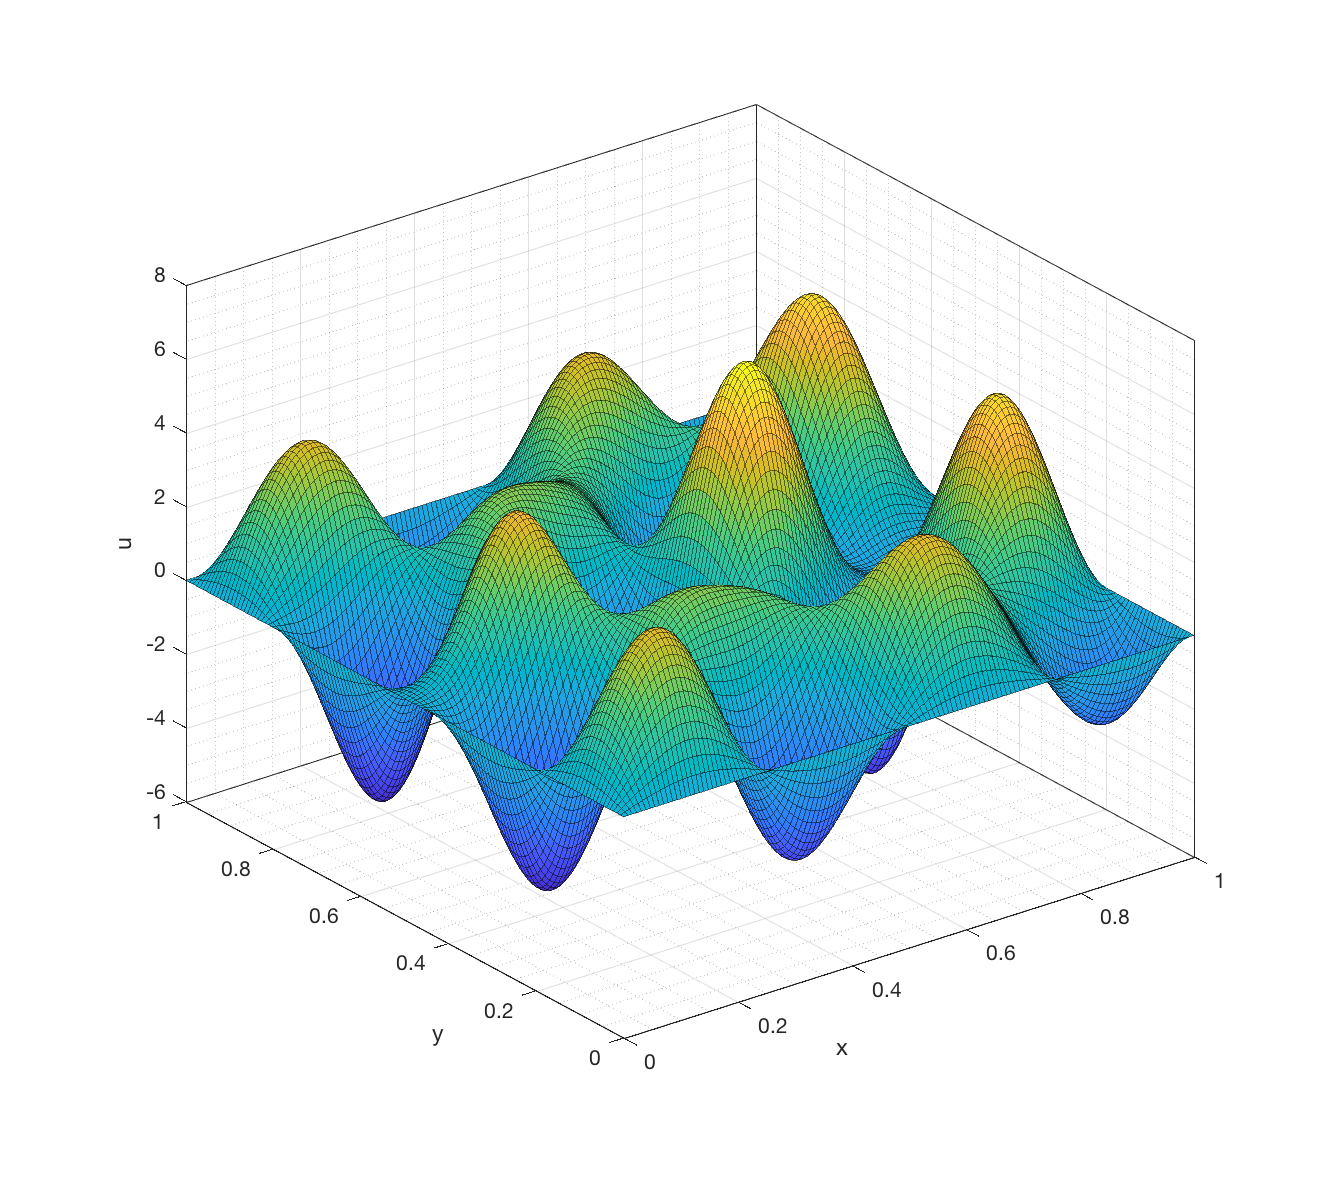
\includegraphics[width = 0.9\linewidth]{title_img}
	\end{center}
\end{figure}

\vspace{80pt}

\newpage

\tableofcontents

\newpage

\section{Model Problems}

\subsection{Wave Equation}

The \textit{first} model problem consists of:
\begin{itemize}
	\item the two-dimensional second-order linear partial differential equation:
	\begin{equation}
	\nabla^2 u + k^2u = k^2x
	\end{equation}
	\item the domain:
	\begin{equation}
	\Omega(x,y) \in [0, 1] \times [0, 1]
	\end{equation}
	\item the boundary conditions:
	\begin{equation}
	u \big|_{\partial \Omega} = 0
	\end{equation}
\end{itemize}

The physical model of the wave equation is that of:
\begin{itemize}
	\begin{spacing}{0.5}
	\item forced vibration of a square membrane
	\item wave propagation of perturbations on a normalized Euclidean $\mathbb{R}^2$ space
	\end{spacing}
\end{itemize}

\subsection{Diffusion Equation}

The \textit{second} model problem consists of:
\begin{itemize}
	\item the two-dimensional second-order linear partial differential equation:
	\begin{equation}
	-\nabla^2 u + k^2u = k^2x
	\end{equation}
	\item the domain:
	\begin{equation}
	\Omega(x,y) \in [0, 1] \times [0, 1]
	\end{equation}
	\item the boundary conditions:
	\begin{equation}
	u \big|_{\partial \Omega} = 0
	\end{equation}
\end{itemize}

The physical model of the diffusion equation is that of:
\begin{itemize}
	\begin{spacing}{0.5}
		\item electrical conduction through a medium that has isotropic electrical conductivity
		\item magnetism of a material that has isotropic magnetic permeability
		\item thermal conduction through a material that has isotropic thermal conductivity
		\item diffusion through a fluid that has isotropic diffusivity
	\end{spacing}
\end{itemize}

\newpage

\section{Analytical Solutions}

\subsection{Analytical Solution of the Wave Equation}

The 2D wave equation, solution domain, and boundary conditions for the \textit{first} model problem are:
\begin{equation}
\psder{u}{x} + \psder{u}{y} + k^2u = k^2x
\end{equation}
\begin{equation}
\Omega(x,y) \in [0, 1] \times [0, 1]
\end{equation}
\begin{equation}
u \big|_{\partial \Omega} = 0
\end{equation}

Employing a set of basis coefficients, $a_i$, and a set of basis functions, $\varphi_i$, we will build the solution to $u(x ,y)$. For our basis functions, we will choose a Fourier double sine series in $x$ and $y$ as a solution to the wave equation giving:
\begin{equation}
u(x,y) = \sum_{i=1}^{\infty} a_{i} \varphi_i
\end{equation}
\begin{equation}
u(x,y) = \sum_{n=1}^{\infty} \sum_{m=1}^{\infty} \underbrace{a_{m,n}}_{a_i} \underbrace{\sin(n\pi x)\sin(m\pi y)}_{\varphi_i}
\end{equation}

By writing in the above form, we assume the existence of $\Omega$ as a Hilbert space $H$ equipped with an inner product. Application of the Galerkin orthogonality condition for our partial differential equation means that the residual form of the partial differential equation, $R(x, y)$, must be orthogonal for every basis function over the entire solution domain, or that:
\begin{equation}
\int_{\Omega}(R(x,y)) \varphi_m d\Omega = 0
\end{equation}
\begin{equation}
\int_{\Omega}\left(\psder{u}{x} + \psder{u}{y} + k^2u - k^2x\right) \varphi_m d\Omega = 0
\end{equation}

Using our above expression for $u(x,y)$ and the principle of orthogonality over the entire solution domain, we may extract a representation for the coefficients of Fourier double sine series assuming their minimization over the entire integral. This takes the form:
\begin{equation}
u(x,y) = \sum_{n=1}^{\infty} \sum_{m=1}^{\infty} a_{m,n} \sin(n\pi x)\sin(m\pi y)
\end{equation}
\begin{equation}
a_{m,n} = 4 \int_{0}^{1} \int_{0}^{1} \sin(n\pi x)\sin(m\pi y) dy dx
\end{equation}

Evaluating the coefficient integral over the domain, we may write the complete solution as:
\begin{equation}
u(x,y) = \sum_{n=1}^{\infty} \sum_{m=1}^{\infty} \frac{4k^2[1-\cos(n\pi)][1-\cos(m\pi)]}{n\pi m\pi\{k^2-\pi^2[(n\pi)^2+(m\pi)^2]\}}  x\sin(n\pi x)\sin(m\pi y)
\end{equation}

\newpage

\subsection{Analytical Solution of the Diffusion Equation}

The 2D diffusion equation, solution domain, and boundary conditions for the \textit{first} model problem are:
\begin{equation}
-\psder{u}{x} - \psder{u}{y} + k^2u = k^2x
\end{equation}
\begin{equation}
\Omega(x,y) \in [0, 1] \times [0, 1]
\end{equation}
\begin{equation}
u \big|_{\partial \Omega} = 0
\end{equation}

Employing a set of basis coefficients, $a_i$, and a set of basis functions, $\varphi_i$, we will build the solution to $u(x ,y)$. For our basis functions, we will choose a Fourier double sine series in $x$ and $y$ as a solution to the wave equation giving:
\begin{equation}
u(x,y) = \sum_{i=1}^{\infty} a_{i} \varphi_i
\end{equation}
\begin{equation}
u(x,y) = \sum_{n=1}^{\infty} \sum_{m=1}^{\infty} \underbrace{a_{m,n}}_{a_i} \underbrace{\sin(n\pi x)\sin(m\pi y)}_{\varphi_i}
\end{equation}

By writing in the above form, we assume the existence of $\Omega$ as a Hilbert space $H$ equipped with an inner product. Application of the Galerkin orthogonality condition for our partial differential equation means that the residual form of the partial differential equation, $R(x, y)$, must be orthogonal for every basis function over the entire solution domain, or that:
\begin{equation}
\int_{\Omega}(R(x,y)) \varphi_m d\Omega = 0
\end{equation}
\begin{equation}
\int_{\Omega}\left(-\psder{u}{x} - \psder{u}{y} + k^2u - k^2x\right) \varphi_m d\Omega = 0
\end{equation}

Using our above expression for $u(x,y)$ and the principle of orthogonality over the entire solution domain, we may extract a representation for the coefficients of Fourier double sine series assuming their minimization over the entire integral. This takes the form:
\begin{equation}
u(x,y) = \sum_{n=1}^{\infty} \sum_{m=1}^{\infty} a_{m,n} \sin(n\pi x)\sin(m\pi y)
\end{equation}
\begin{equation}
a_{m,n} = 4 \int_{0}^{1} \int_{0}^{1} \sin(n\pi x)\sin(m\pi y) dy dx
\end{equation}

Evaluating the coefficient integral over the domain, we may write the complete solution as:
\begin{equation}
u(x,y) = \sum_{n=1}^{\infty} \sum_{m=1}^{\infty} \frac{4k^2[1-\cos(n\pi)][1-\cos(m\pi)]}{n\pi m\pi\{k^2+\pi^2[(n\pi)^2+(m\pi)^2]\}}  x\sin(n\pi x)\sin(m\pi y)
\end{equation}

\newpage

\section{Numerical Methods}

\subsection{2nd-Order Central Difference Scheme Finite Difference Method - Wave Equation}

\subsubsection{Finite Difference Method}

Constructing the standard second-order second partial derivatives with respect to $x$ and $y$ around localized point $u(x,y)=u_{i,j}$ we have:
\begin{equation}
\label{eqn:2ox}
\psder{u}{x}\Big|_{i,j} = \frac{u_{i-1, j} - 2u_{i,j} + u_{i+1, j}}{\Delta x^2} + \mathcal{O}(\Delta x^2)
\end{equation}
\begin{equation}
\label{eqn:2oy}
\psder{u}{y}\Big|_{i,j} = \frac{u_{i, j-1} - 2u_{i,j} + u_{i, j+1}}{\Delta y^2} + \mathcal{O}(\Delta y^2)
\end{equation}

\subsubsection{Discretized Differential Equation}

The wave equation is:
\begin{equation}
\psder{u}{x} + \psder{u}{y} +  k^2u = k^2x
\end{equation}
Discretizing a uniform mesh ($\Delta x = \Delta y$) using Equations \ref{eqn:2ox} and \ref{eqn:2oy}, we get a \textbf{5-point stencil} in $x$ and $y$ which is equal to $k^2 \Delta x^2 x_i$:

\begin{table}[H]
	\begin{tabular}{ccc}
		 & $u_{i, j+1}$ &  \\
		$u_{i-1, j}$ & $(-4+k^2\Delta x^2)u_{i, j}$ & $u_{i+1, j}$ \\
		 & $u_{i, j-1}$ & 
	\end{tabular}
\end{table}

\subsubsection{Discretized Extraction Formula}
The quantity of interest is the derivative with respect to $x$ at the center of the right boundary , $u_x(1, \tfrac{1}{2})$.
The Taylor series in around this point yields:
\begin{equation}
u(1-\Delta x, \tfrac{1}{2}) = u(1, \tfrac{1}{2}) - \Delta x \pder{u}{x}\Big|_{\left(1, \tfrac{1}{2}\right)} + \frac{\Delta x^2}{2} \psder{u}{x}\Big|_{\left(1, \tfrac{1}{2}\right)} + \mathcal{O}(\Delta x^3)
\end{equation}
From our boundary condition $u \big|_{\partial \Omega} = 0 $ we can cancel the $u$ term:
\begin{equation}
u(1-\Delta x, \tfrac{1}{2}) = - \Delta x \pder{u}{x}\Big|_{\left(1, \tfrac{1}{2}\right)} + \frac{\Delta x^2}{2} \psder{u}{x}\Big|_{\left(1, \tfrac{1}{2}\right)} + \mathcal{O}(\Delta x^3)
\end{equation}
From our differential equation $\psder{u}{x} + \psder{u}{y} +  k^2u = k^2x$ we can cancel the rewrite the $\psder{u}{x}$ term:
\begin{equation}
u(1-\Delta x, \tfrac{1}{2}) = - \Delta x \pder{u}{x}\Big|_{\left(1, \tfrac{1}{2}\right)} + \frac{\Delta x^2}{2} \left(- \psder{u}{y} -  k^2u + k^2x\right)\Big|_{\left(1, \tfrac{1}{2}\right)} + \mathcal{O}(\Delta x^3)
\end{equation}
Again from our boundary condition $u \big|_{\partial \Omega} = 0 $ we can cancel the $u$ term and the $\psder{u}{y}$ term and impose the proper $x$ value:
\begin{equation}
u(1-\Delta x, \tfrac{1}{2}) = - \Delta x \pder{u}{x}\Big|_{\left(1, \tfrac{1}{2}\right)} + \frac{k^2\Delta x^2}{2} + \mathcal{O}(\Delta x^3)
\end{equation}
Now, rearranging for the quantity of interest, we have our discretized extraction formula, which is second-order accurate:
\begin{equation}
\pder{u}{x}\Big|_{\left(1, \tfrac{1}{2}\right)} = \frac{k^2\Delta x}{2} -\frac{u(1-\Delta x, \tfrac{1}{2})}{\Delta x}
\end{equation}

\newpage

\subsection{4th-Order Central Difference Scheme Finite Difference Method - Wave Equation}

\subsubsection{Finite Difference Method}
Constructing the standard fourth-order second partial derivatives with respect to $x$ and $y$ around localized point $u(x,y)=u_{i,j}$ we have:
\begin{equation}
\label{eqn:4ox}
\psder{u}{x}\Big|_{i,j} = \frac{u_{i-1, j} - 2u_{i,j} + u_{i+1, j}}{\Delta x^2} - \frac{\Delta x^2}{12} \pfder{u}{x}\Big|_{i,j} + \mathcal{O}(\Delta x^4)
\end{equation}
\begin{equation}
\label{eqn:4oy}
\psder{u}{y}\Big|_{i,j} = \frac{u_{i, j-1} - 2u_{i,j} + u_{i, j+1}}{\Delta y^2} - \frac{\Delta y^2}{12} \pfder{u}{y}\Big|_{i,j} + \mathcal{O}(\Delta y^4)
\end{equation}

In order to make the expressions more implicit, the fourth derivatives must be generalized. Thus, returning to the differential equation and we take two additional derivatives with respect to $x$ and $y$. Since the problem is independent and sufficiently smooth, the order of differentiation does not change the problem, and we achieve:
\begin{equation}
\pfder{u}{x}=  -\frac{\partial^4 u}{\partial x^2 \partial y^2} -k^2\psder{u}{x}
\end{equation}
\begin{equation}
\pfder{u}{y}=  -\frac{\partial^4 u}{\partial y^2 \partial x^2} -k^2\psder{u}{y}
\end{equation}
with:
\begin{equation}
\frac{\partial^4 u}{\partial y^2 \partial x^2} = \frac{\partial^4 u}{\partial x^2 \partial y^2}
\end{equation}
A discretization of the fourth-order mixed derivative in $x$ and $y$ is:
\begin{equation}
\frac{\partial^4 u}{\partial x^2 \partial y^2} = \frac{1}{\Delta x^2 \Delta y^2}\left[(u_{i-1, j-1}-2u_{i, j-1}+u_{i+1, j-1})-2(u_{i-1, j}-2u_{i, j}+u_{i+1, j})+(u_{i-1, j+1}-2u_{i, j+1}+u_{i+1, j+1})\right]
\end{equation}
Replacing the two higher-order derivatives, we achieve the fourth-order-accurate approximations:
\begin{equation}
\psder{u}{x}\Big|_{i,j} = \frac{u_{i-1, j} - 2u_{i,j} + u_{i+1, j}}{\Delta x^2} - \frac{\Delta x^2}{12} \left[\psder{}{y}\left(\psder{u}{x}\right) + k^2\psder{u}{x}\right]\Big|_{i,j} + \mathcal{O}(\Delta x^4)
\end{equation}
\begin{equation}
\psder{u}{y}\Big|_{i,j} = \frac{u_{i, j-1} - 2u_{i,j} + u_{i, j+1}}{\Delta y^2} - \frac{\Delta y^2}{12} \left[\psder{}{x}\left(\psder{u}{y}\right) + k^2\psder{u}{y}\right]\Big|_{i,j} + \mathcal{O}(\Delta y^4)
\end{equation}

\subsubsection{Discretized Differential Equation}

The wave equation is:
\begin{equation}
\psder{u}{x} + \psder{u}{y} +  k^2u = k^2x
\end{equation}
Discretizing a uniform mesh using Equations \ref{eqn:4ox} and \ref{eqn:4oy}, we get a \textbf{9-point stencil} in $x$ and $y$ which is equal to $k^2\Delta x^2 x_i$:

\begin{table}[H]
	\begin{tabular}{ccc}
		$\tfrac{2}{12}u_{i-1, j+1}$ & $\tfrac{1}{12}(8+k^2\Delta x^2)u_{i, j+1}$ & $\tfrac{2}{12}u_{i+1, j+1}$  \\
		$\tfrac{1}{12}(8+k^2\Delta x^2)u_{i-1, j}$ & $\tfrac{1}{12}(-40+8k^2\Delta x^2)u_{i, j}$ & $\tfrac{1}{12}(8+k^2\Delta x^2)u_{i+1, j}$ \\
		$\tfrac{2}{12}u_{i-1, j-1}$ & $\tfrac{1}{12}(8+k^2\Delta x^2)u_{i, j-1}$ & $\tfrac{2}{12}u_{i+1, j-1}$
	\end{tabular}
\end{table}

\subsection{2nd-Order Central Difference Scheme Finite Difference Method - Diffusion Equation}

\subsubsection{Finite Difference Method}

Constructing the standard second-order second partial derivatives with respect to $x$ and $y$ around localized point $u(x,y)=u_{i,j}$ we have:
\begin{equation}
\label{eqn:2oxd}
\psder{u}{x}\Big|_{i,j} = \frac{u_{i-1, j} - 2u_{i,j} + u_{i+1, j}}{\Delta x^2} + \mathcal{O}(\Delta x^2)
\end{equation}
\begin{equation}
\label{eqn:2oyd}
\psder{u}{y}\Big|_{i,j} = \frac{u_{i, j-1} - 2u_{i,j} + u_{i, j+1}}{\Delta y^2} + \mathcal{O}(\Delta y^2)
\end{equation}

\subsubsection{Discretized Differential Equation}

The diffusion equation is:
\begin{equation}
-\psder{u}{x} - \psder{u}{y} +  k^2u = k^2x
\end{equation}
Discretizing a uniform mesh ($\Delta x = \Delta y$) using Equations \ref{eqn:2oxd} and \ref{eqn:2oyd}, we get a \textbf{5-point stencil} in $x$ and $y$ which is equal to $k^2 \Delta x^2 x_i$:

\begin{table}[H]
	\begin{tabular}{ccc}
		& $-u_{i, j+1}$ &  \\
		$-u_{i-1, j}$ & $(4+k^2\Delta x^2)u_{i, j}$ & $-u_{i+1, j}$ \\
		& $-u_{i, j-1}$ & 
	\end{tabular}
\end{table}

\subsubsection{Discretized Extraction Formula}
The quantity of interest is the derivative with respect to $x$ at the center of the right boundary , $u_x(1, \tfrac{1}{2})$.
The Taylor series in around this point yields:
\begin{equation}
u(1-\Delta x, \tfrac{1}{2}) = u(1, \tfrac{1}{2}) - \Delta x \pder{u}{x}\Big|_{\left(1, \tfrac{1}{2}\right)} + \frac{\Delta x^2}{2} \psder{u}{x}\Big|_{\left(1, \tfrac{1}{2}\right)} + \mathcal{O}(\Delta x^3)
\end{equation}
From our boundary condition $u \big|_{\partial \Omega} = 0 $ we can cancel the $u$ term:
\begin{equation}
u(1-\Delta x, \tfrac{1}{2}) = - \Delta x \pder{u}{x}\Big|_{\left(1, \tfrac{1}{2}\right)} + \frac{\Delta x^2}{2} \psder{u}{x}\Big|_{\left(1, \tfrac{1}{2}\right)} + \mathcal{O}(\Delta x^3)
\end{equation}
From our differential equation $-\psder{u}{x} - \psder{u}{y} +  k^2u = k^2x$ we can cancel the rewrite the $\psder{u}{x}$ term:
\begin{equation}
u(1-\Delta x, \tfrac{1}{2}) = - \Delta x \pder{u}{x}\Big|_{\left(1, \tfrac{1}{2}\right)} + \frac{\Delta x^2}{2} \left(- \psder{u}{y} +  k^2u - k^2x\right)\Big|_{\left(1, \tfrac{1}{2}\right)} + \mathcal{O}(\Delta x^3)
\end{equation}
Again from our boundary condition $u \big|_{\partial \Omega} = 0 $ we can cancel the $u$ term and the $\psder{u}{y}$ term and impose the proper $x$ value:
\begin{equation}
u(1-\Delta x, \tfrac{1}{2}) = - \Delta x \pder{u}{x}\Big|_{\left(1, \tfrac{1}{2}\right)} - \frac{k^2\Delta x^2}{2} + \mathcal{O}(\Delta x^3)
\end{equation}
Now, rearranging for the quantity of interest, we have our discretized extraction formula, which is second-order accurate:
\begin{equation}
\pder{u}{x}\Big|_{\left(1, \tfrac{1}{2}\right)} = -\frac{k^2\Delta x}{2} -\frac{u(1-\Delta x, \tfrac{1}{2})}{\Delta x}
\end{equation}

\newpage

\subsection{4th-Order Central Difference Scheme Finite Difference Method - Diffusion Equation}

\subsubsection{Finite Difference Method}
Constructing the standard fourth-order second partial derivatives with respect to $x$ and $y$ around localized point $u(x,y)=u_{i,j}$ we have:
\begin{equation}
\label{eqn:4oxd}
\psder{u}{x}\Big|_{i,j} = \frac{u_{i-1, j} - 2u_{i,j} + u_{i+1, j}}{\Delta x^2} - \frac{\Delta x^2}{12} \pfder{u}{x}\Big|_{i,j} + \mathcal{O}(\Delta x^4)
\end{equation}
\begin{equation}
\label{eqn:4oyd}
\psder{u}{y}\Big|_{i,j} = \frac{u_{i, j-1} - 2u_{i,j} + u_{i, j+1}}{\Delta y^2} - \frac{\Delta y^2}{12} \pfder{u}{y}\Big|_{i,j} + \mathcal{O}(\Delta y^4)
\end{equation}

In order to make the expressions more implicit, the fourth derivatives must be generalized. Thus, returning to the differential equation and we take two additional derivatives with respect to $x$ and $y$. Since the problem is independent and sufficiently smooth, the order of differentiation does not change the problem, and we achieve:
\begin{equation}
\pfder{u}{x}=  -\frac{\partial^4 u}{\partial x^2 \partial y^2} +k^2\psder{u}{x}
\end{equation}
\begin{equation}
\pfder{u}{y}=  -\frac{\partial^4 u}{\partial y^2 \partial x^2} +k^2\psder{u}{y}
\end{equation}
with:
\begin{equation}
\frac{\partial^4 u}{\partial y^2 \partial x^2} = \frac{\partial^4 u}{\partial x^2 \partial y^2}
\end{equation}
A discretization of the fourth-order mixed derivative in $x$ and $y$ is:
\begin{equation}
\frac{\partial^4 u}{\partial x^2 \partial y^2} = \frac{1}{\Delta x^2 \Delta y^2}\left[(u_{i-1, j-1}-2u_{i, j-1}+u_{i+1, j-1})-2(u_{i-1, j}-2u_{i, j}+u_{i+1, j})+(u_{i-1, j+1}-2u_{i, j+1}+u_{i+1, j+1})\right]
\end{equation}
Replacing the two higher-order derivatives, we achieve the fourth-order-accurate approximations:
\begin{equation}
\psder{u}{x}\Big|_{i,j} = \frac{u_{i-1, j} - 2u_{i,j} + u_{i+1, j}}{\Delta x^2} - \frac{\Delta x^2}{12} \left[\psder{}{y}\left(\psder{u}{x}\right) - k^2\psder{u}{x}\right]\Big|_{i,j} + \mathcal{O}(\Delta x^4)
\end{equation}
\begin{equation}
\psder{u}{y}\Big|_{i,j} = \frac{u_{i, j-1} - 2u_{i,j} + u_{i, j+1}}{\Delta y^2} - \frac{\Delta y^2}{12} \left[\psder{}{x}\left(\psder{u}{y}\right) - k^2\psder{u}{y}\right]\Big|_{i,j} + \mathcal{O}(\Delta y^4)
\end{equation}

\subsubsection{Discretized Differential Equation}

The diffusion equation is:
\begin{equation}
- \psder{u}{x} - \psder{u}{y} +  k^2u = k^2x
\end{equation}
Discretizing a uniform mesh using Equations \ref{eqn:4oxd} and \ref{eqn:4oyd}, we get a \textbf{9-point stencil} in $x$ and $y$ which is equal to $k^2\Delta x^2 x_i$:

\begin{table}[H]
	\begin{tabular}{ccc}
		$\tfrac{-2}{12}u_{i-1, j+1}$ & $\tfrac{1}{12}(-8+k^2\Delta x^2)u_{i, j+1}$ & $\tfrac{-2}{12}u_{i+1, j+1}$  \\
		$\tfrac{1}{12}(-8+k^2\Delta x^2)u_{i-1, j}$ & $\tfrac{1}{12}(40+8k^2\Delta x^2)u_{i, j}$ & $\tfrac{1}{12}(-8+k^2\Delta x^2)u_{i+1, j}$ \\
		$\tfrac{-2}{12}u_{i-1, j-1}$ & $\tfrac{1}{12}(-8+k^2\Delta x^2)u_{i, j-1}$ & $\tfrac{-2}{12}u_{i+1, j-1}$
	\end{tabular}
\end{table}

\section{Results}

\subsection{Finite Difference Method -- Solution Results}

\subsubsection{2nd-Order Central Difference Scheme - Wave Equation}

\begin{figure}[H]
	\begin{center}
		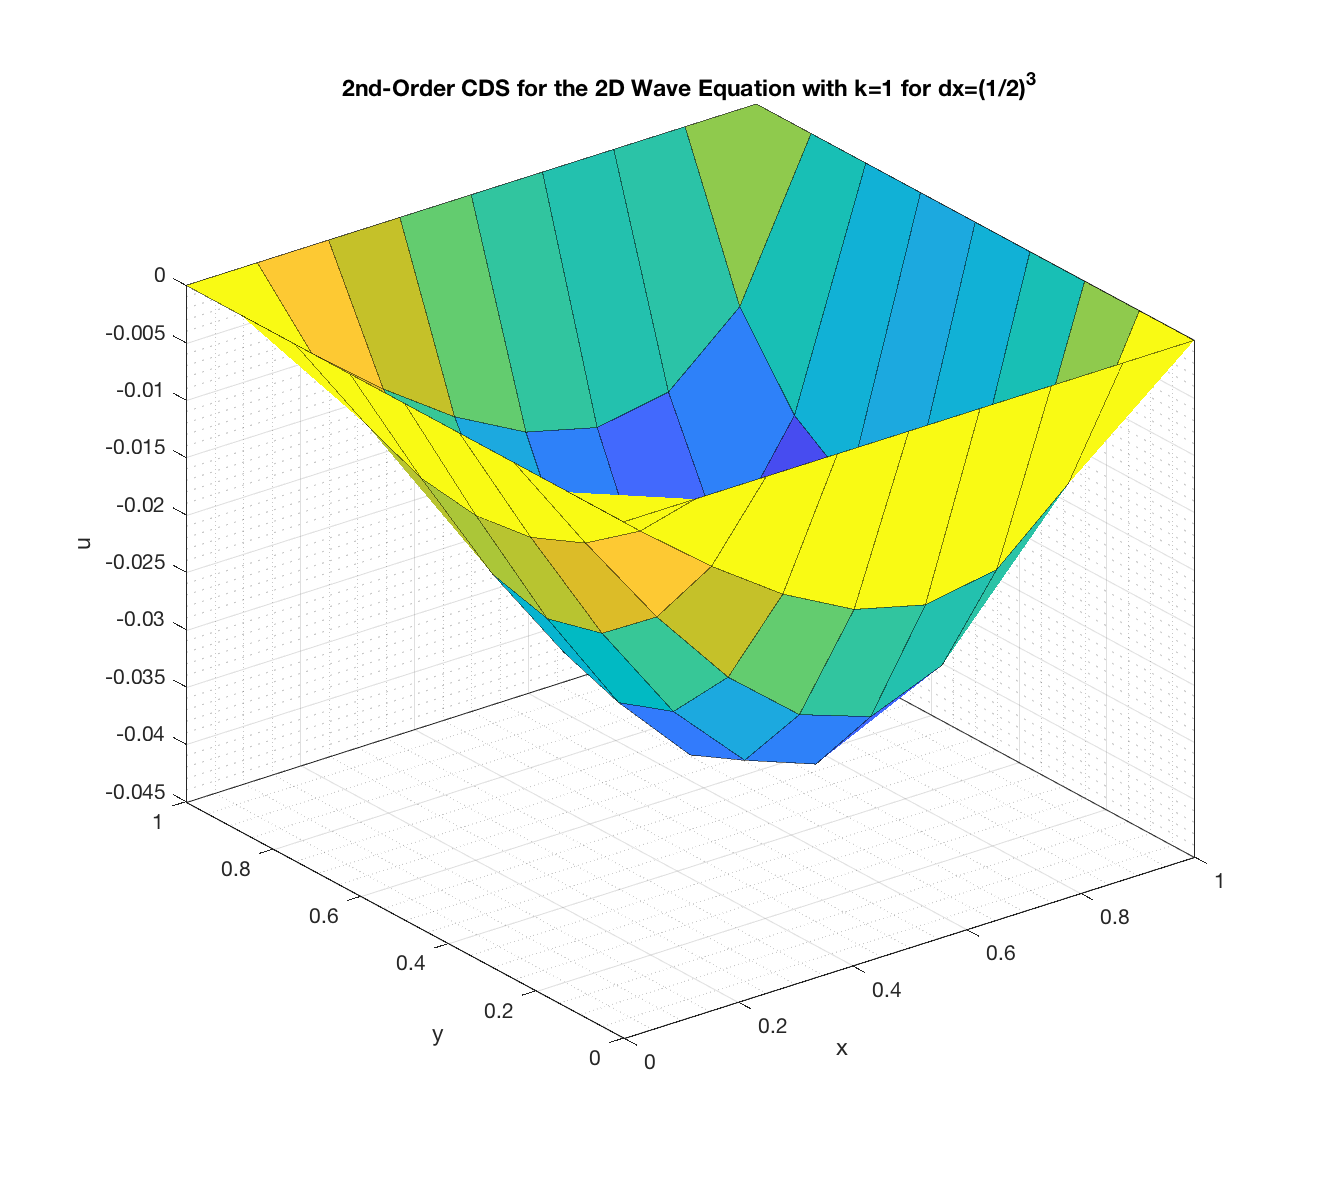
\includegraphics[width = 0.32\linewidth]{surface_plus_order_2_k_1_dx_order_3}
		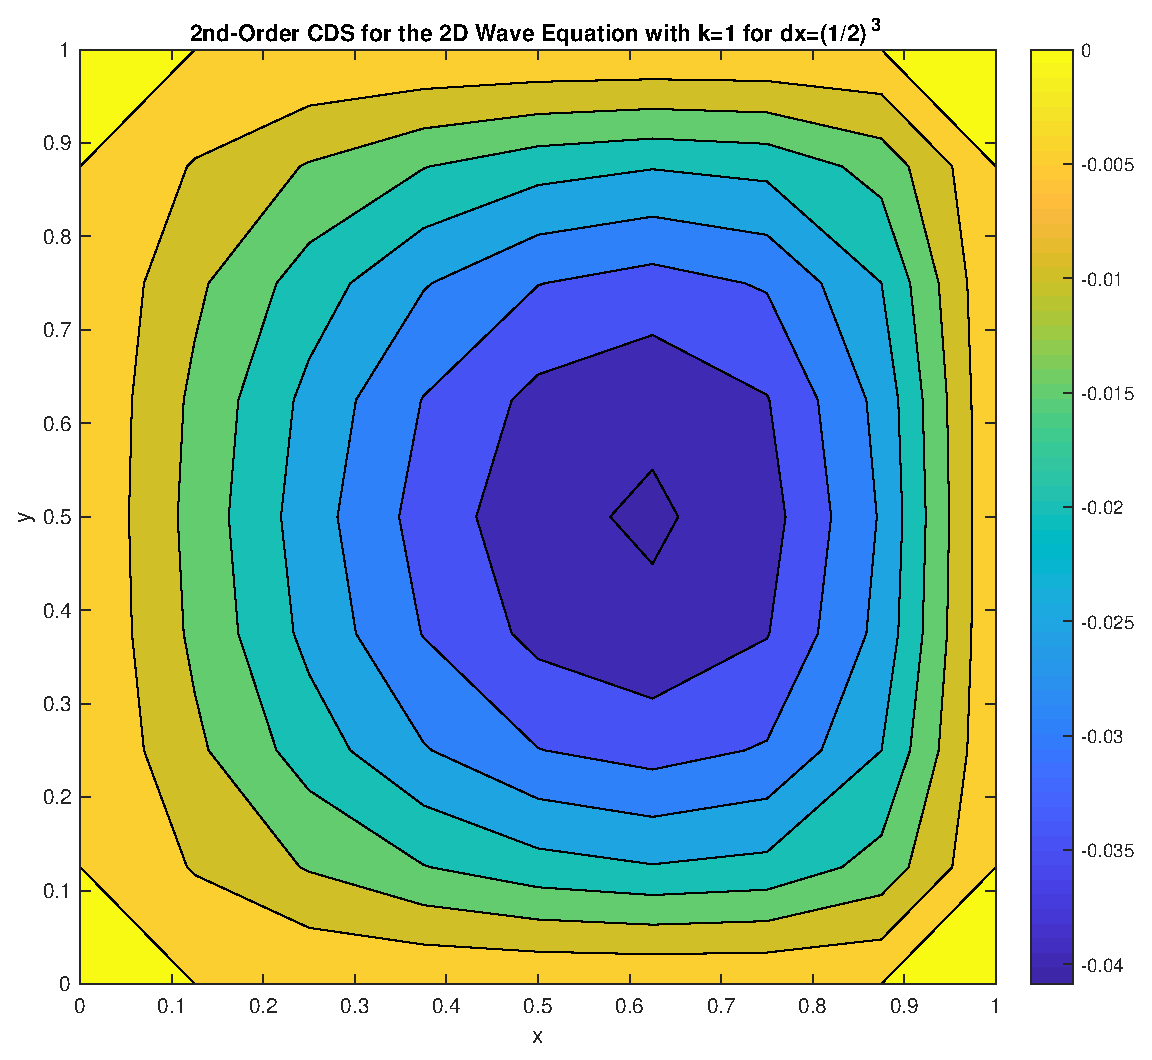
\includegraphics[width = 0.32\linewidth]{contour_plus_order_2_k_1_dx_order_3}
		\caption{2nd-Order CDS for the 2D Wave Equation with $k = 1$ for $\Delta x = (1/2)^3$}
	\end{center}
\end{figure}

\begin{figure}[H]
	\begin{center}
		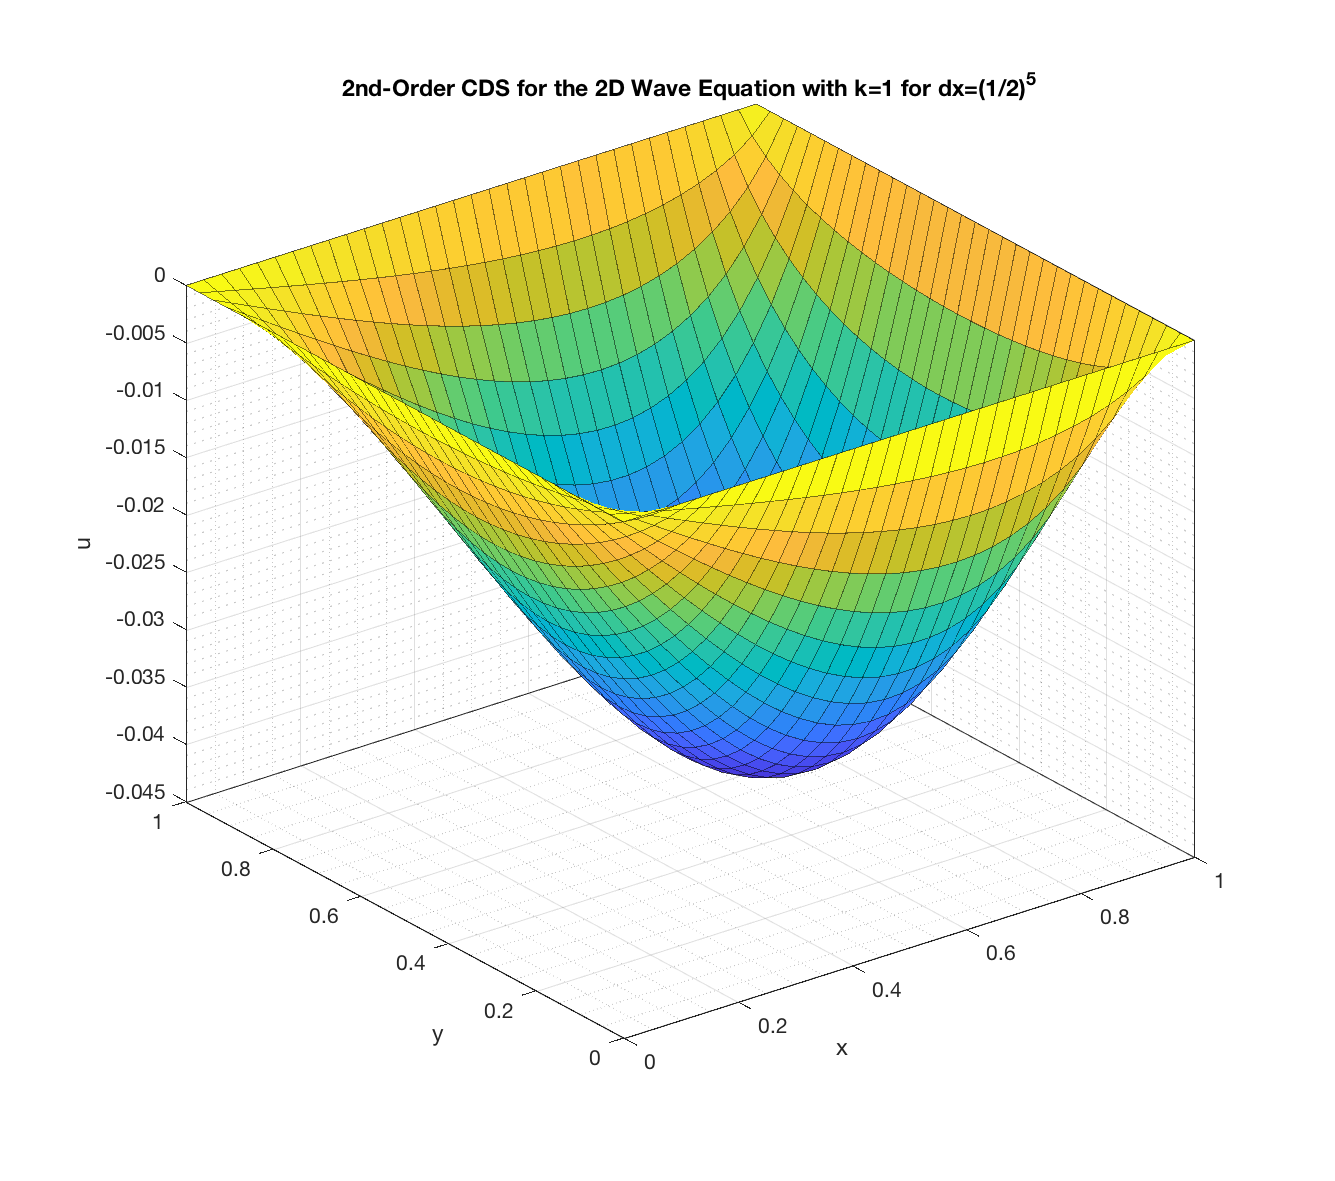
\includegraphics[width = 0.32\linewidth]{surface_plus_order_2_k_1_dx_order_5}
		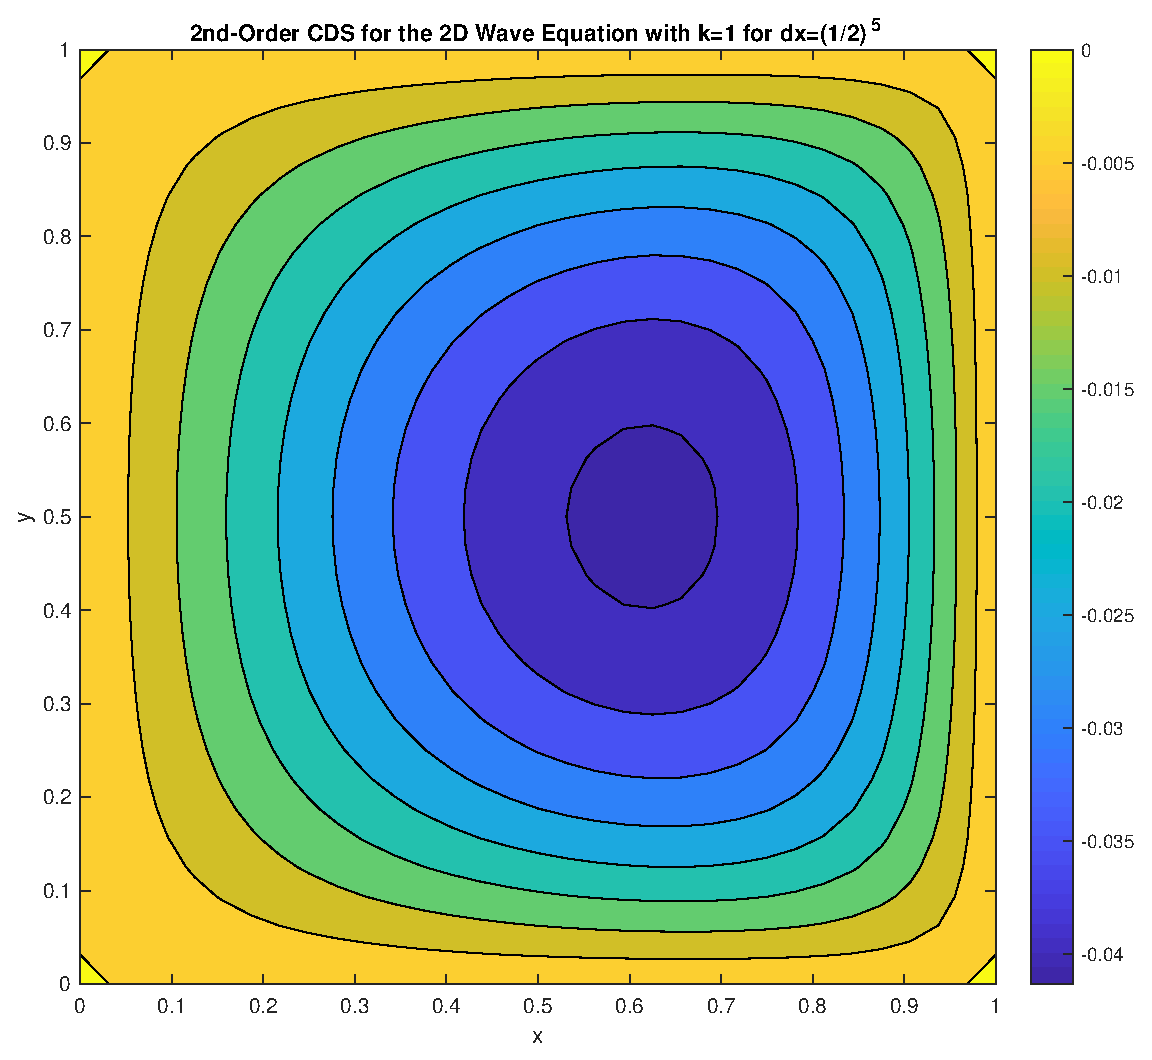
\includegraphics[width = 0.32\linewidth]{contour_plus_order_2_k_1_dx_order_5}
		\caption{2nd-Order CDS for the 2D Wave Equation with $k = 1$ for $\Delta x = (1/2)^5$}
	\end{center}
\end{figure}

\begin{figure}[H]
	\begin{center}
		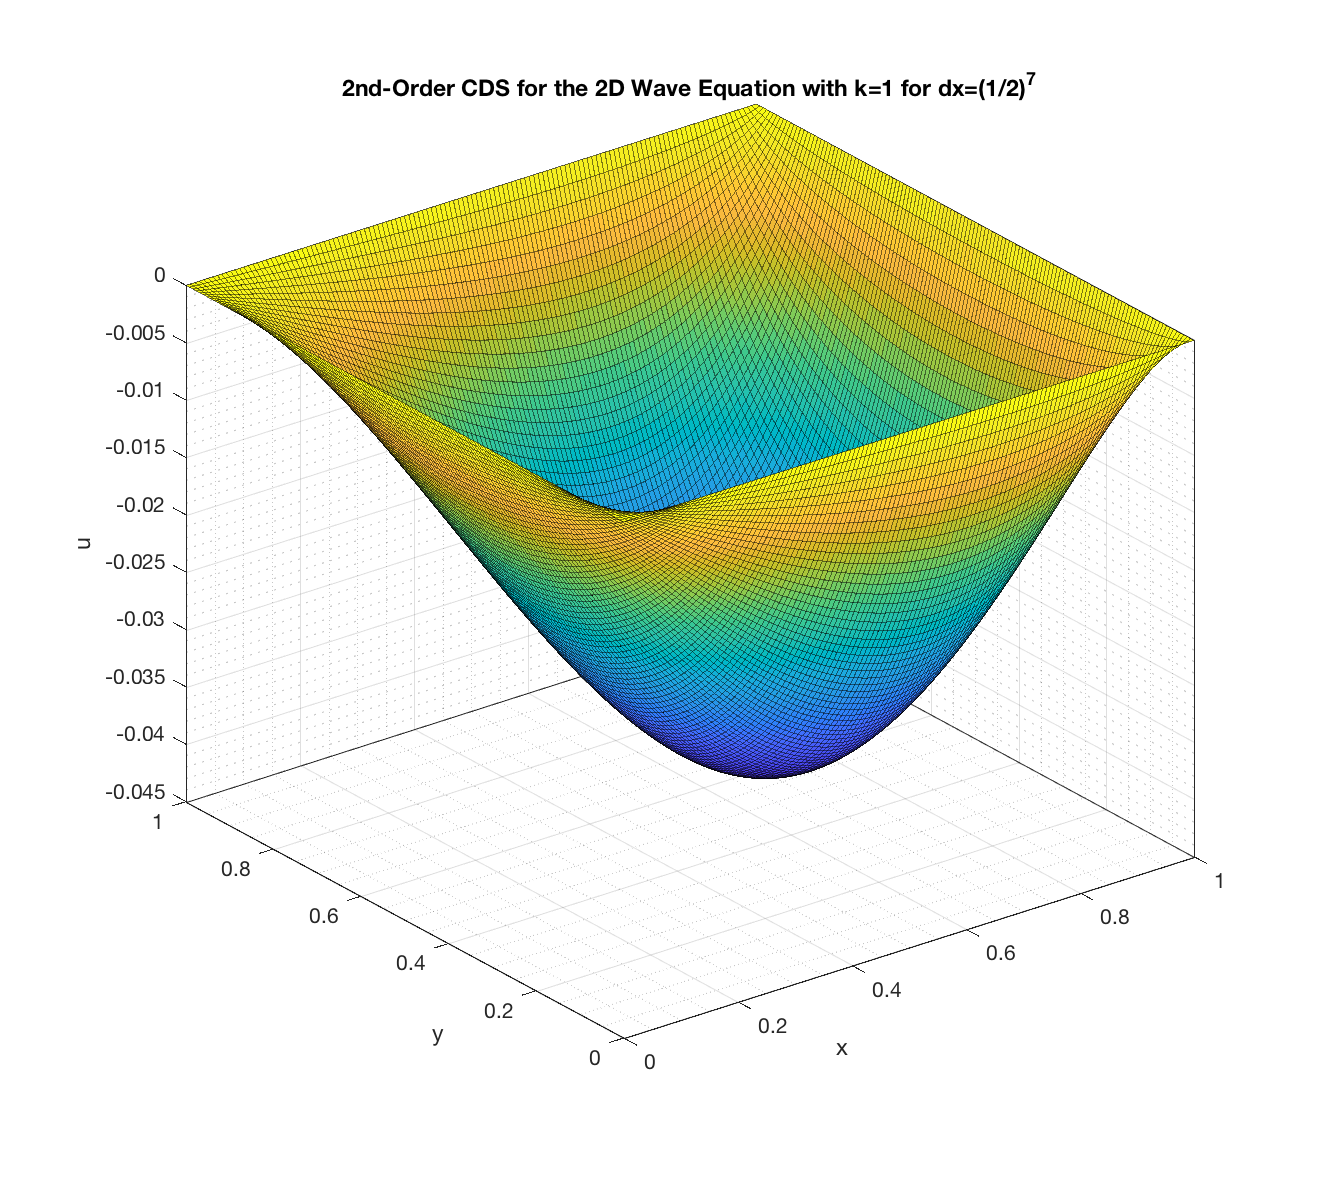
\includegraphics[width = 0.32\linewidth]{surface_plus_order_2_k_1_dx_order_7}
		\includegraphics[width = 0.32\linewidth]{contour_plus_order_2_k_1_dx_order_7}
		\caption{2nd-Order CDS for the 2D Wave Equation with $k = 1$ for $\Delta x = (1/2)^7$}
	\end{center}
\end{figure}

\newpage

\begin{figure}[H]
	\begin{center}
		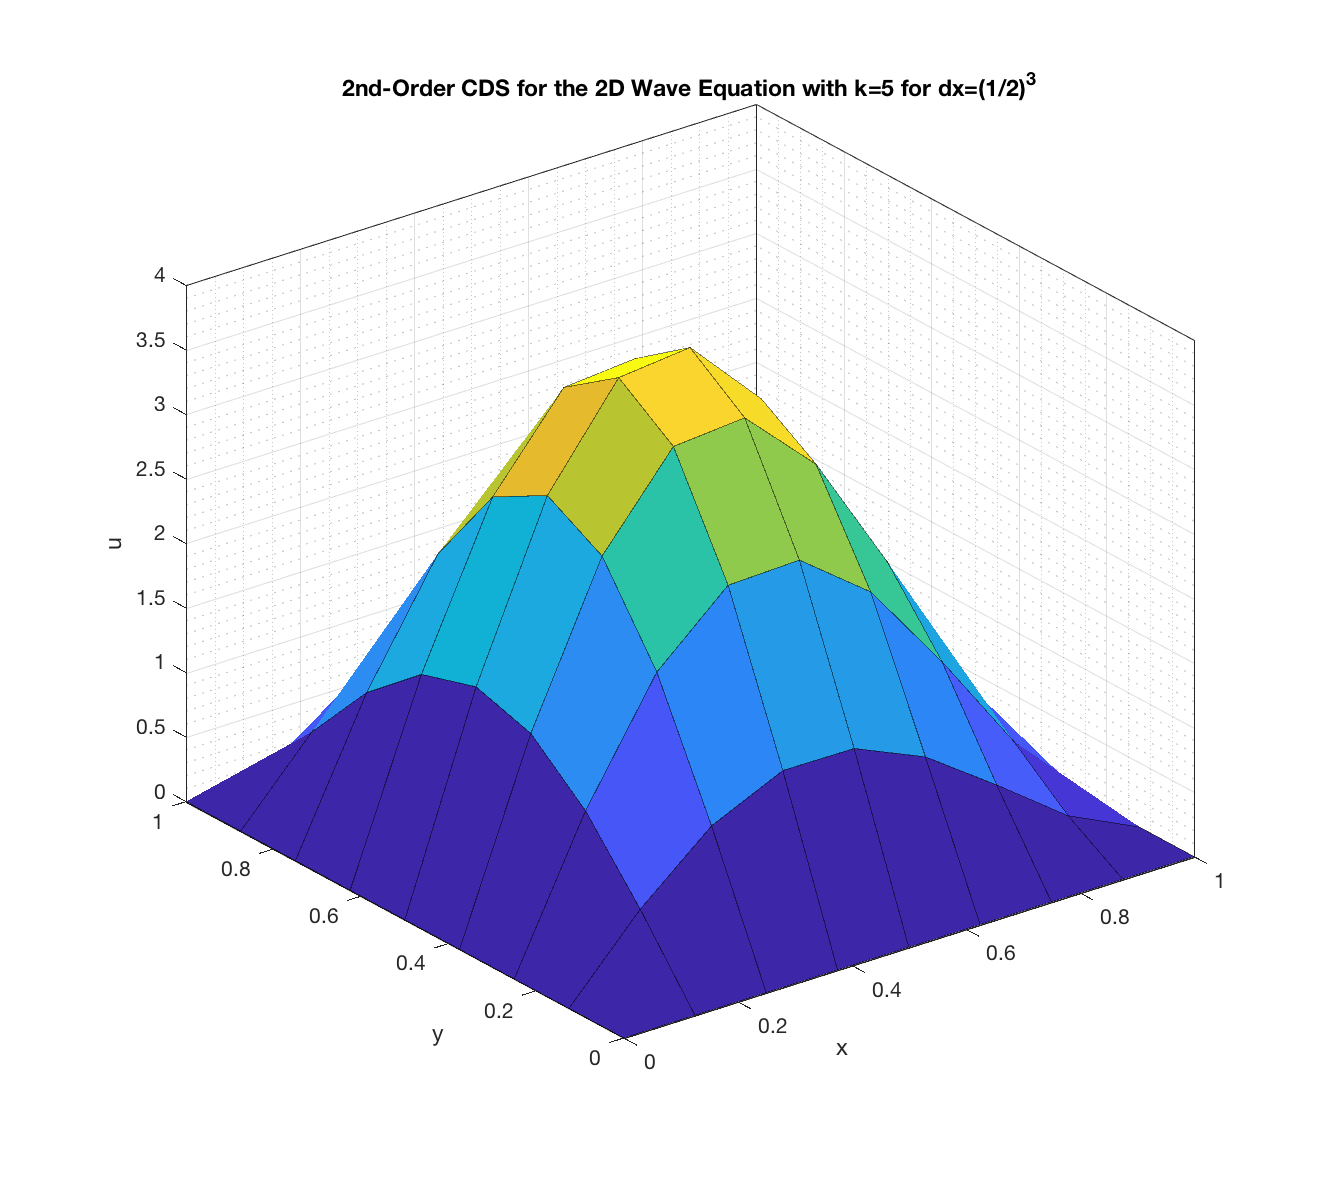
\includegraphics[width = 0.36\linewidth]{surface_plus_order_2_k_5_dx_order_3}
		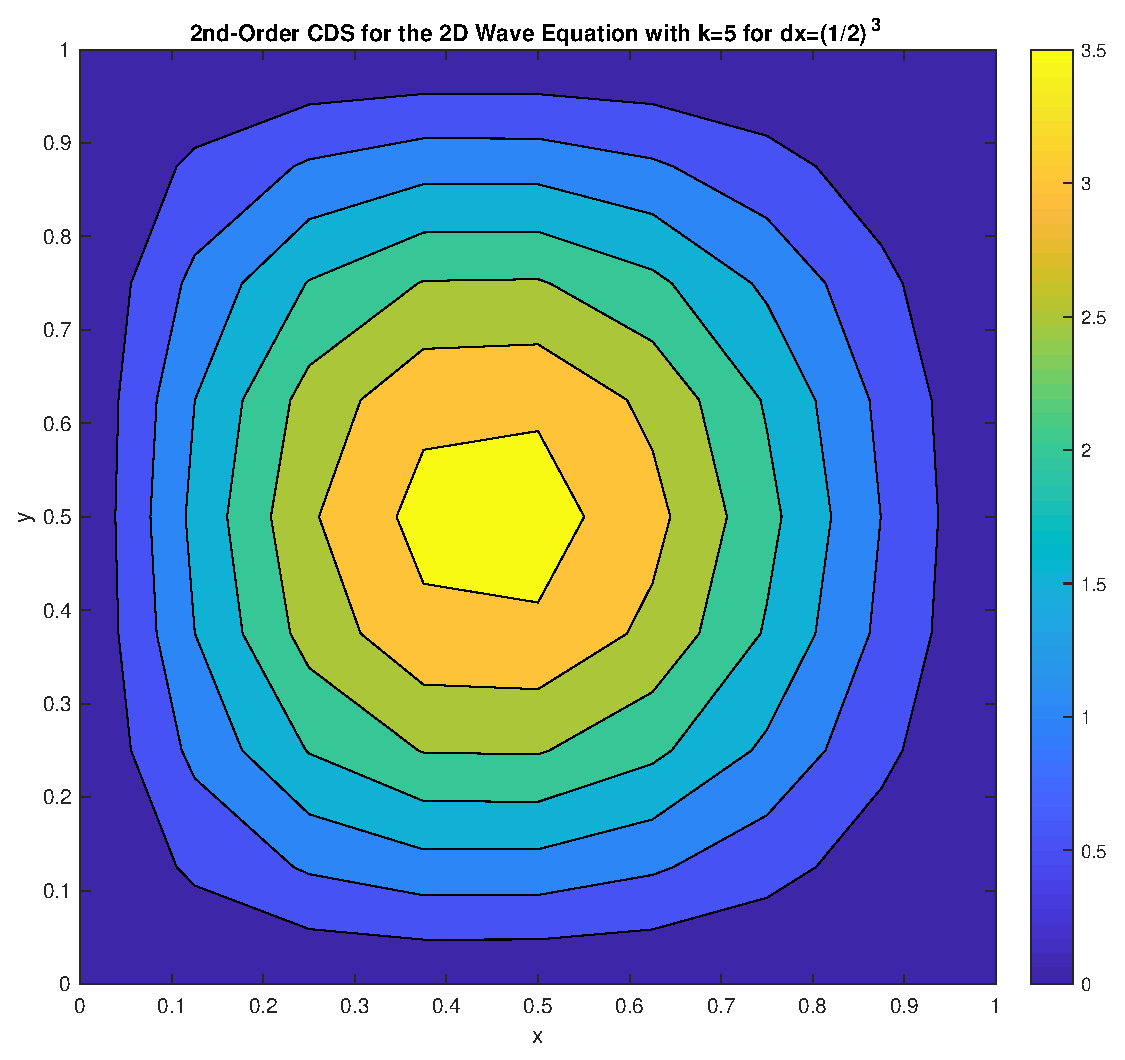
\includegraphics[width = 0.36\linewidth]{contour_plus_order_2_k_5_dx_order_3}
		\caption{2nd-Order CDS for the 2D Wave Equation with $k = 5$ for $\Delta x = (1/2)^3$}
	\end{center}
\end{figure}

\begin{figure}[H]
	\begin{center}
		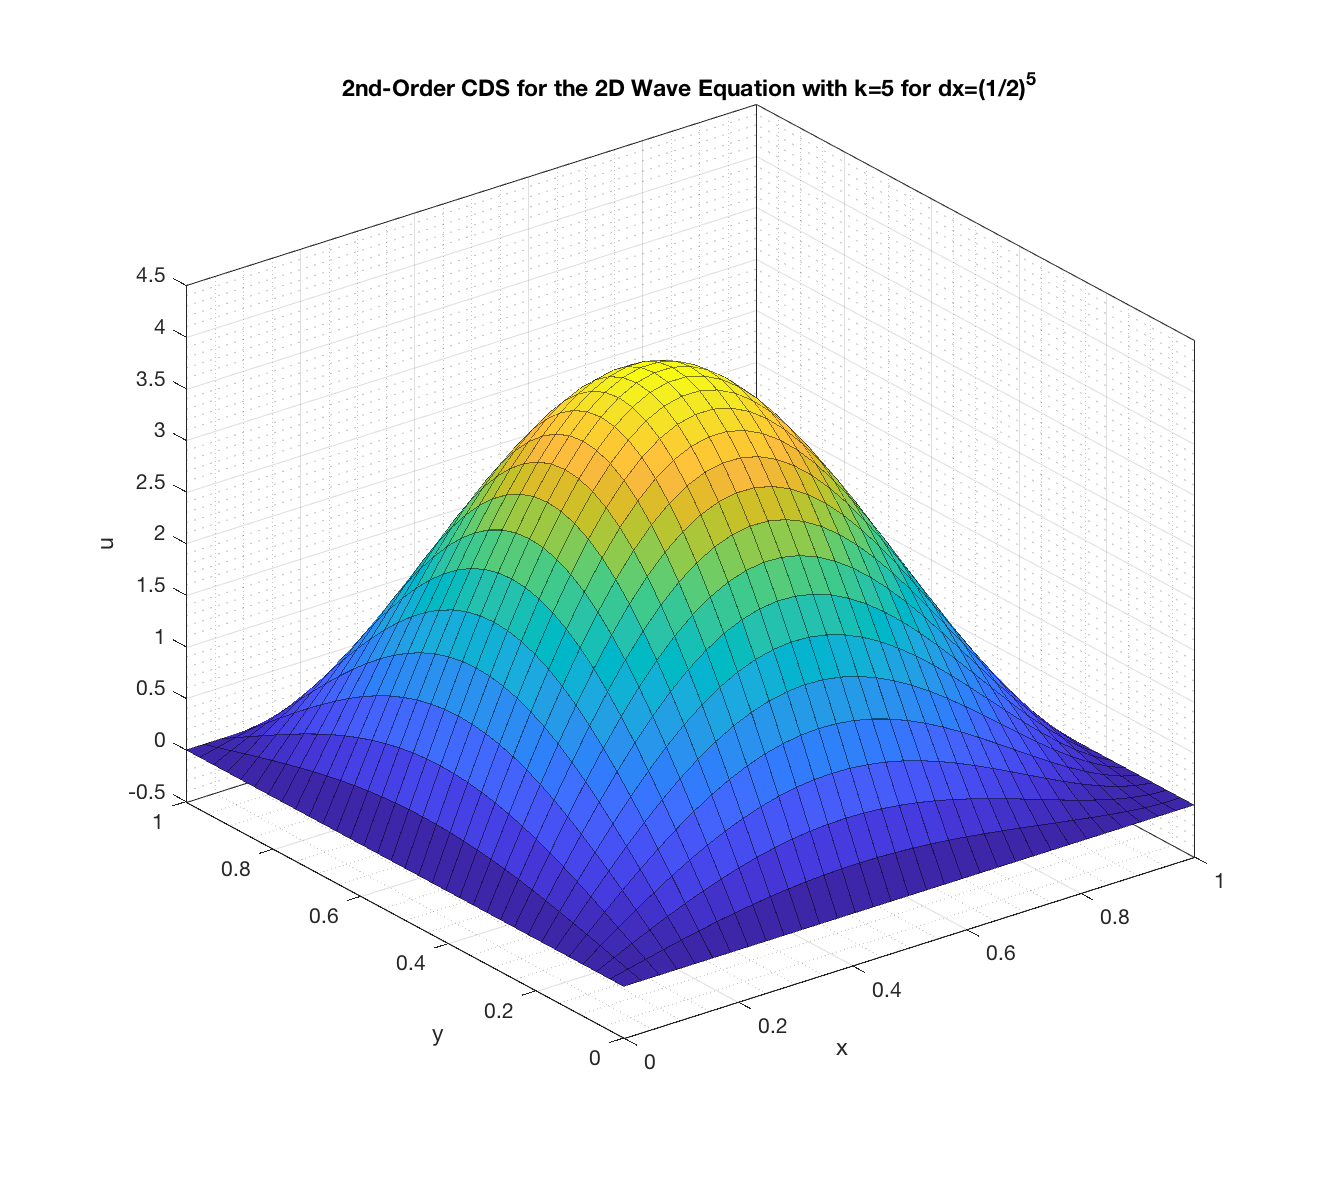
\includegraphics[width = 0.36\linewidth]{surface_plus_order_2_k_5_dx_order_5}
		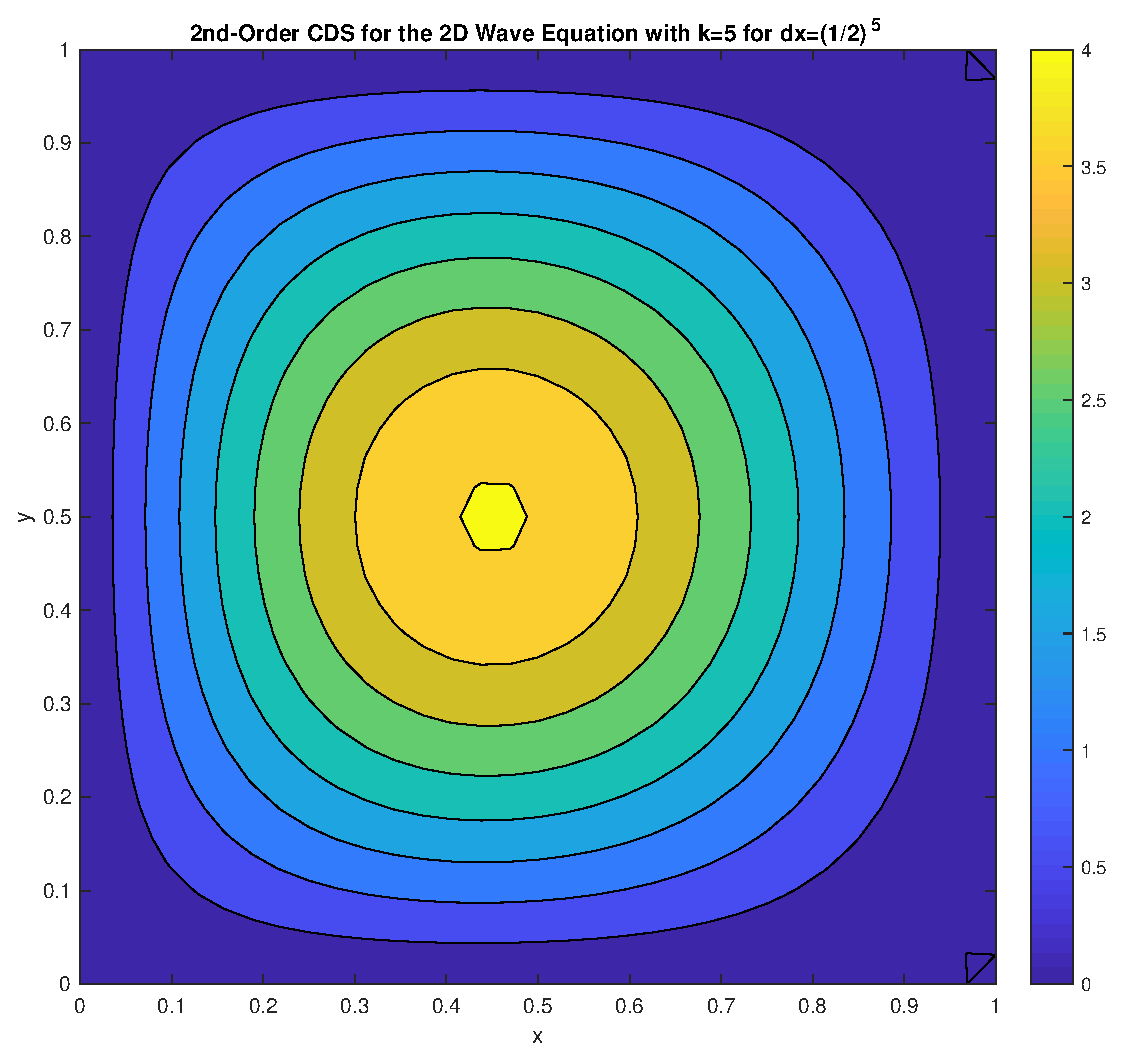
\includegraphics[width = 0.36\linewidth]{contour_plus_order_2_k_5_dx_order_5}
		\caption{2nd-Order CDS for the 2D Wave Equation with $k = 5$ for $\Delta x = (1/2)^5$}
	\end{center}
\end{figure}

\begin{figure}[H]
	\begin{center}
		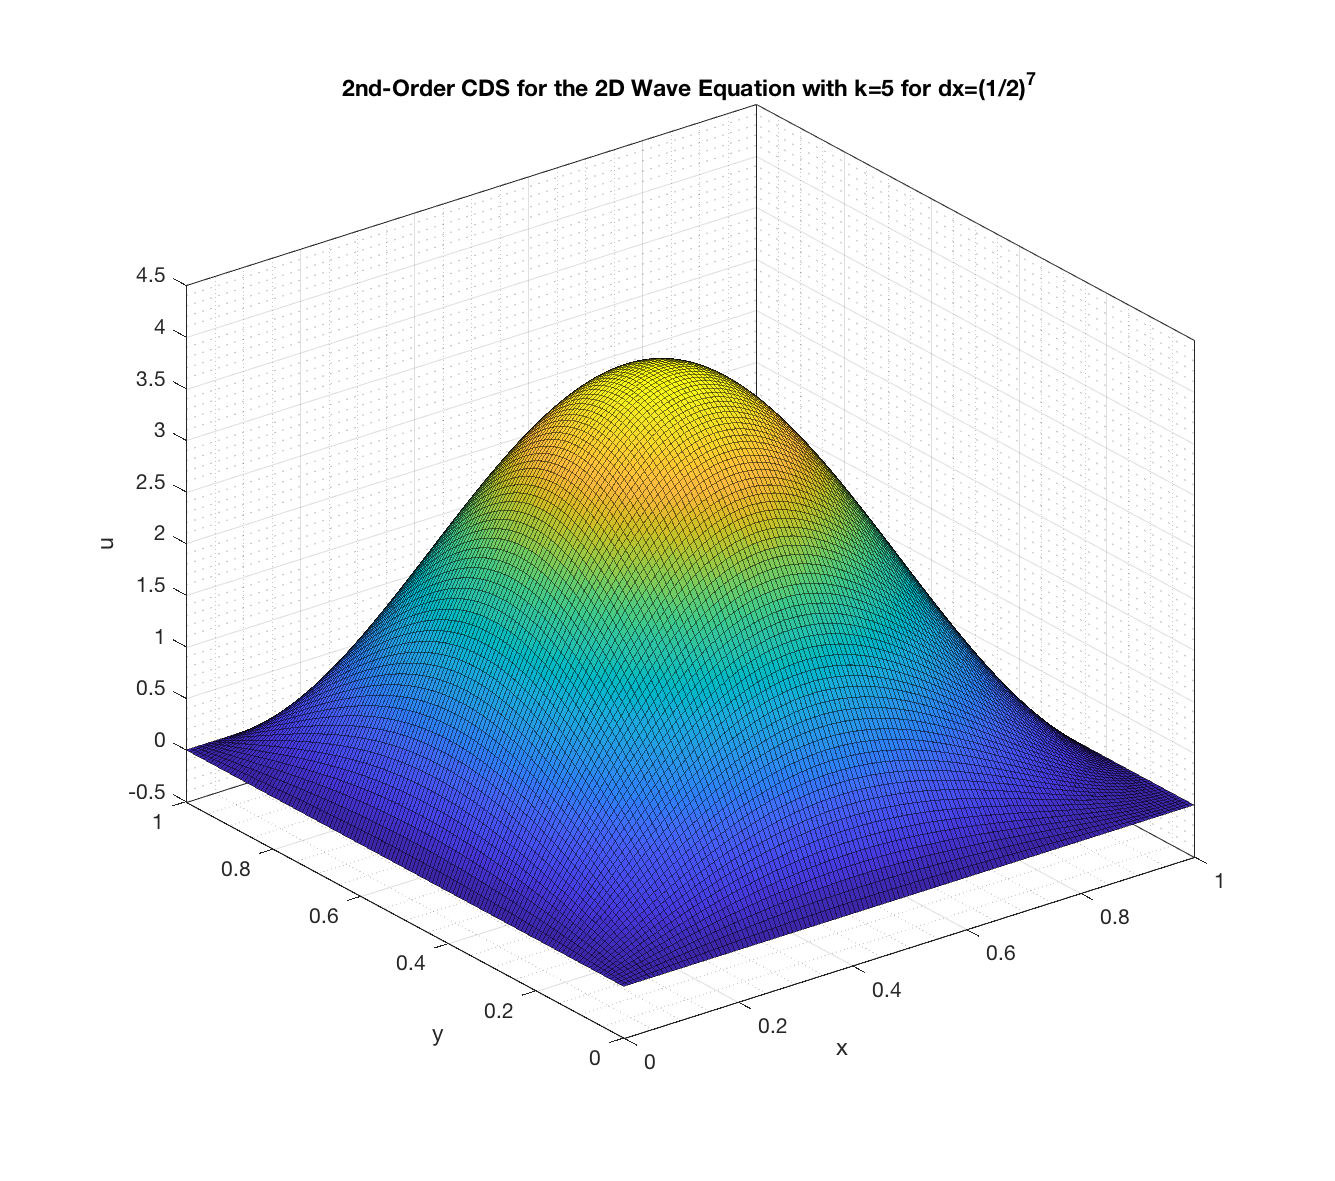
\includegraphics[width = 0.36\linewidth]{surface_plus_order_2_k_5_dx_order_7}
		\includegraphics[width = 0.36\linewidth]{contour_plus_order_2_k_5_dx_order_7}
		\caption{2nd-Order CDS for the 2D Wave Equation with $k = 5$ for $\Delta x = (1/2)^7$}
	\end{center}
\end{figure}

\newpage

\begin{figure}[H]
	\begin{center}
		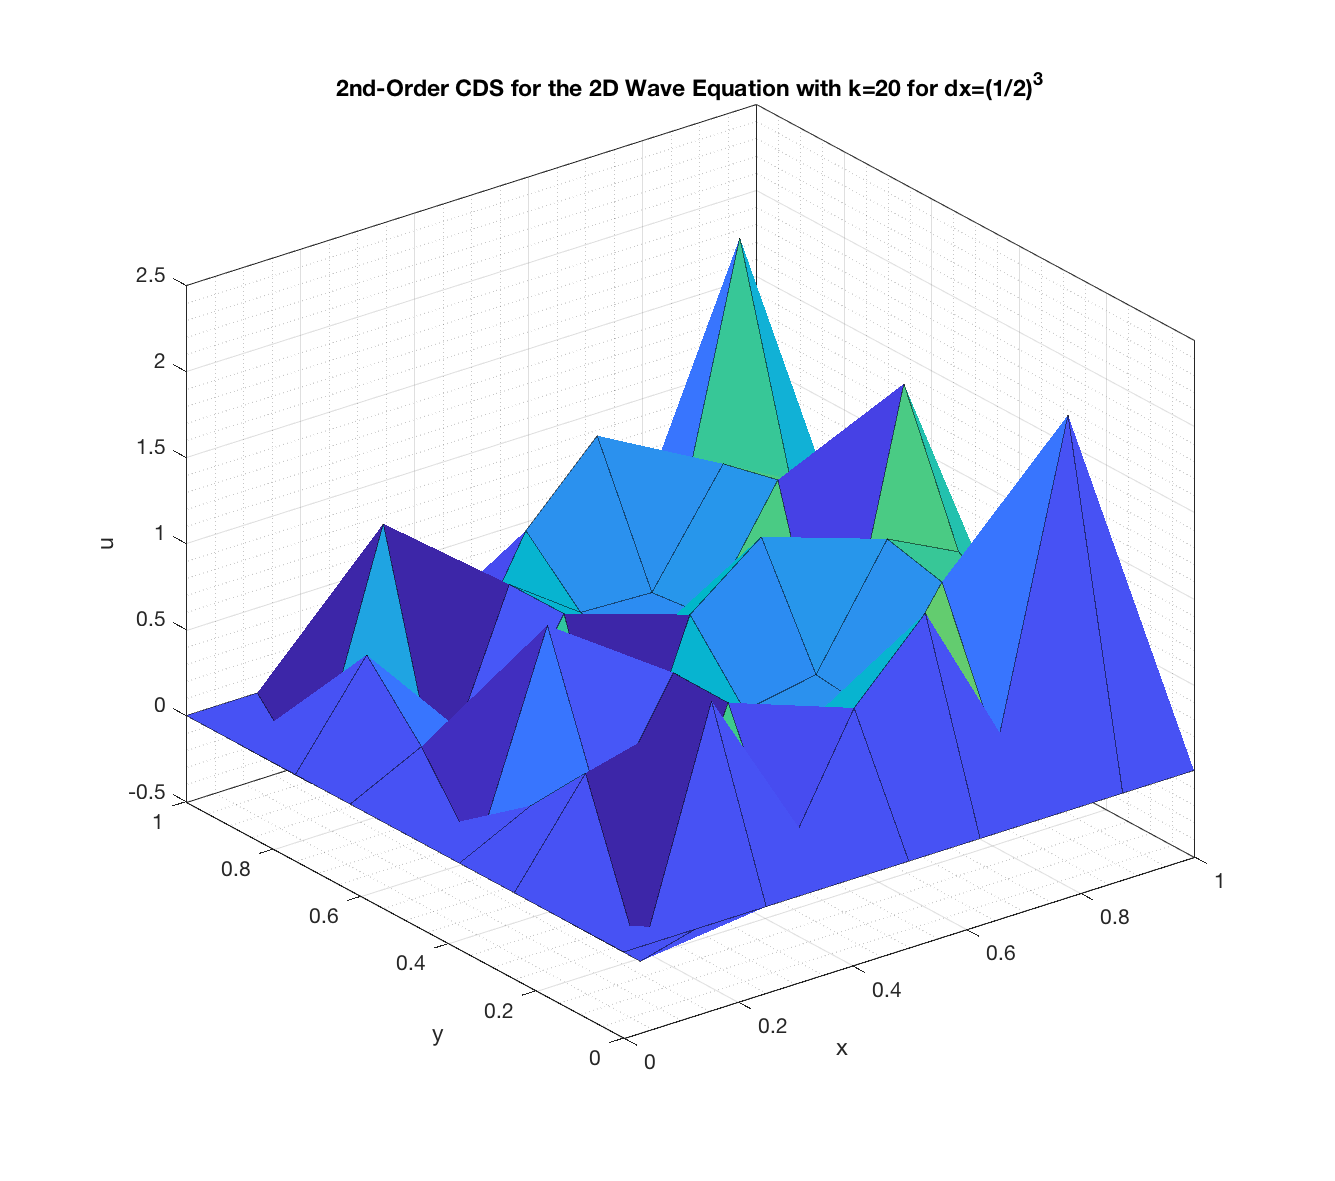
\includegraphics[width = 0.36\linewidth]{surface_plus_order_2_k_20_dx_order_3}
		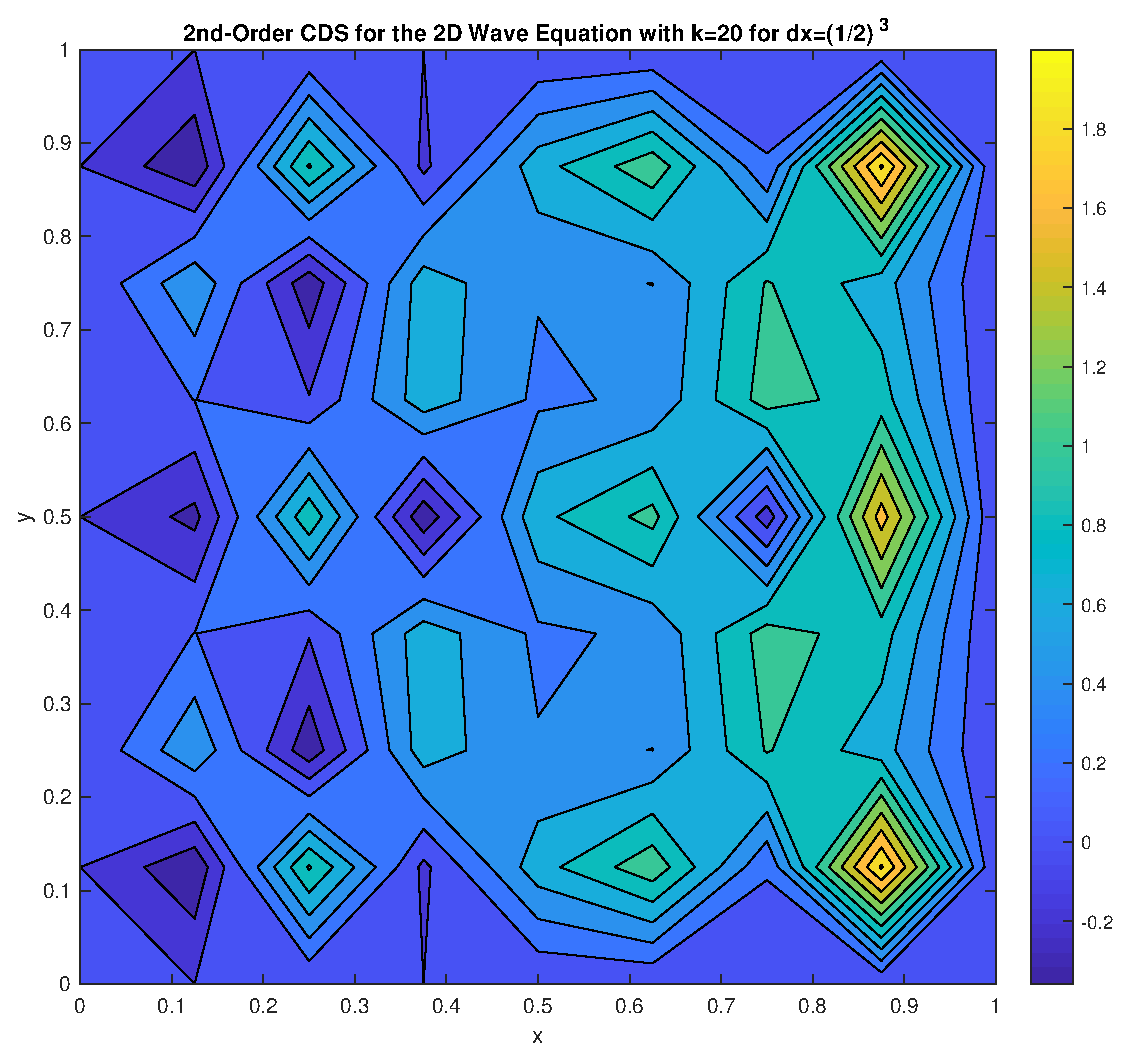
\includegraphics[width = 0.36\linewidth]{contour_plus_order_2_k_20_dx_order_3}
		\caption{2nd-Order CDS for the 2D Wave Equation with $k = 20$ for $\Delta x = (1/2)^3$}
	\end{center}
\end{figure}

\begin{figure}[H]
	\begin{center}
		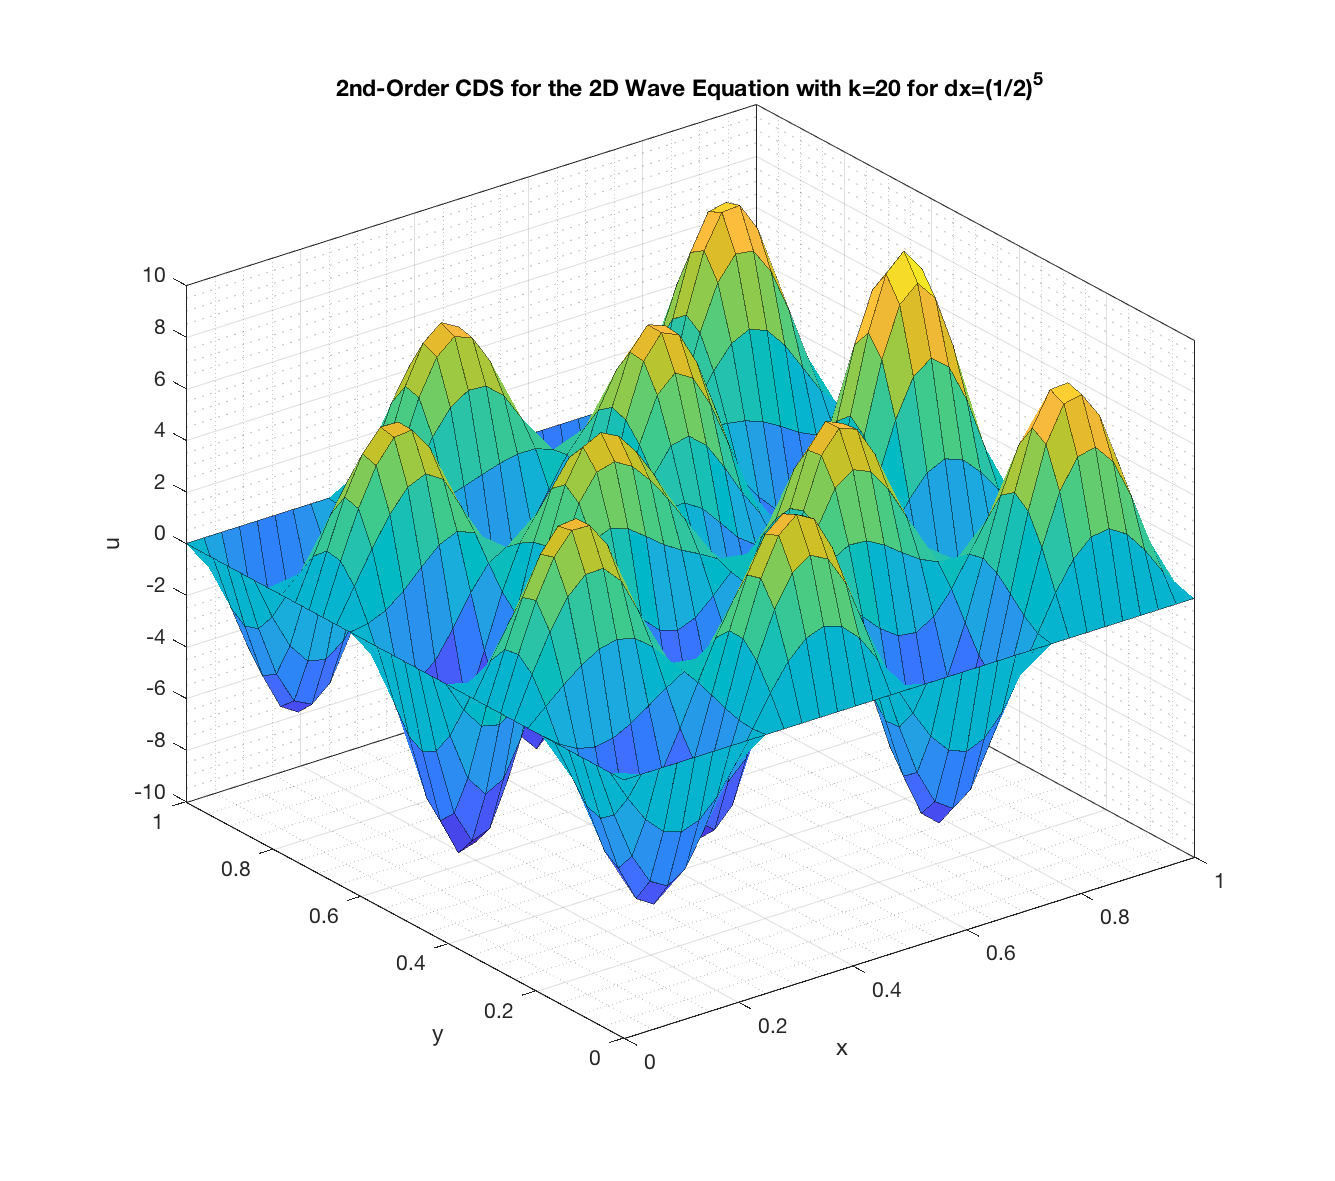
\includegraphics[width = 0.36\linewidth]{surface_plus_order_2_k_20_dx_order_5}
		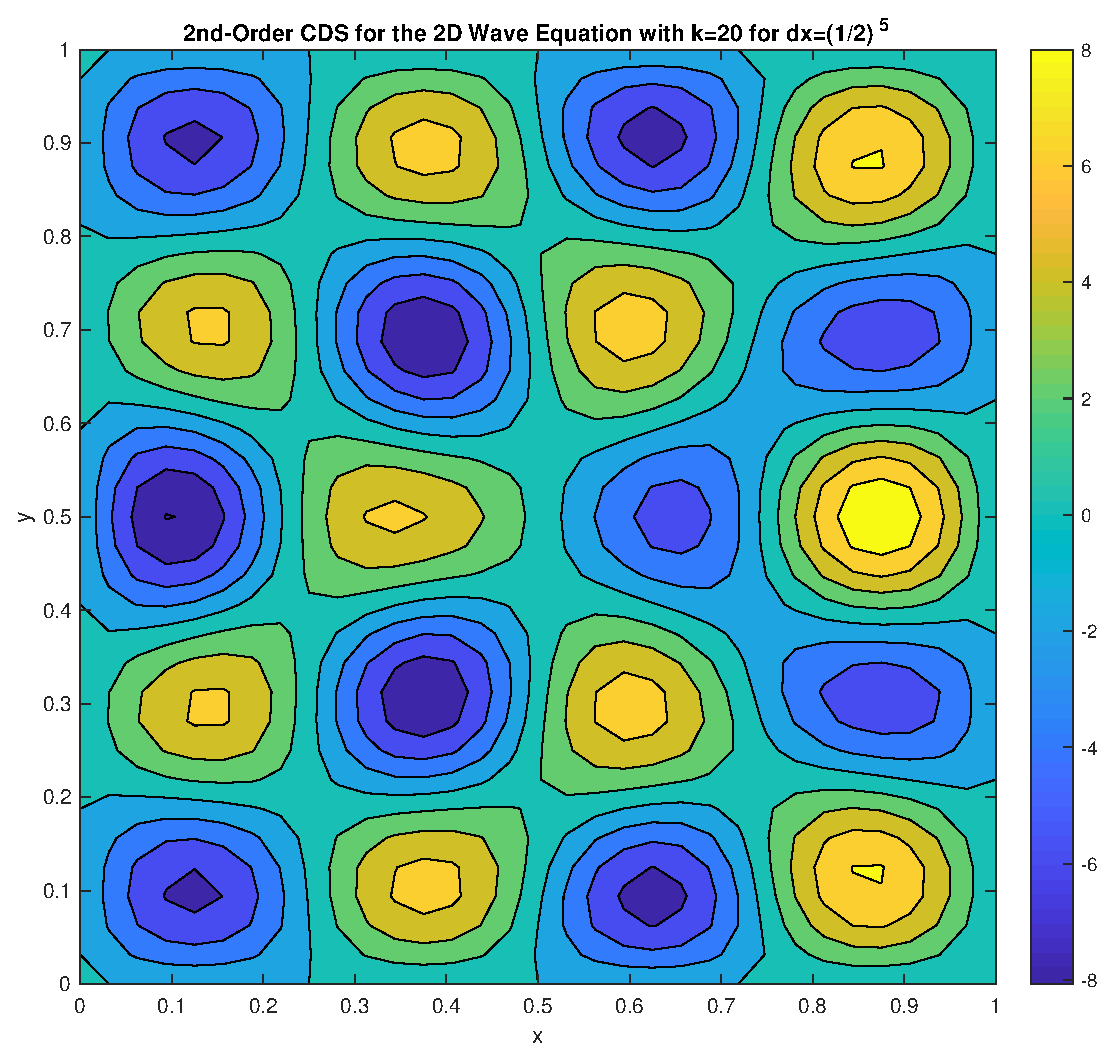
\includegraphics[width = 0.36\linewidth]{contour_plus_order_2_k_20_dx_order_5}
		\caption{2nd-Order CDS for the 2D Wave Equation with $k = 20$ for $\Delta x = (1/2)^5$}
	\end{center}
\end{figure}

\begin{figure}[H]
	\begin{center}
		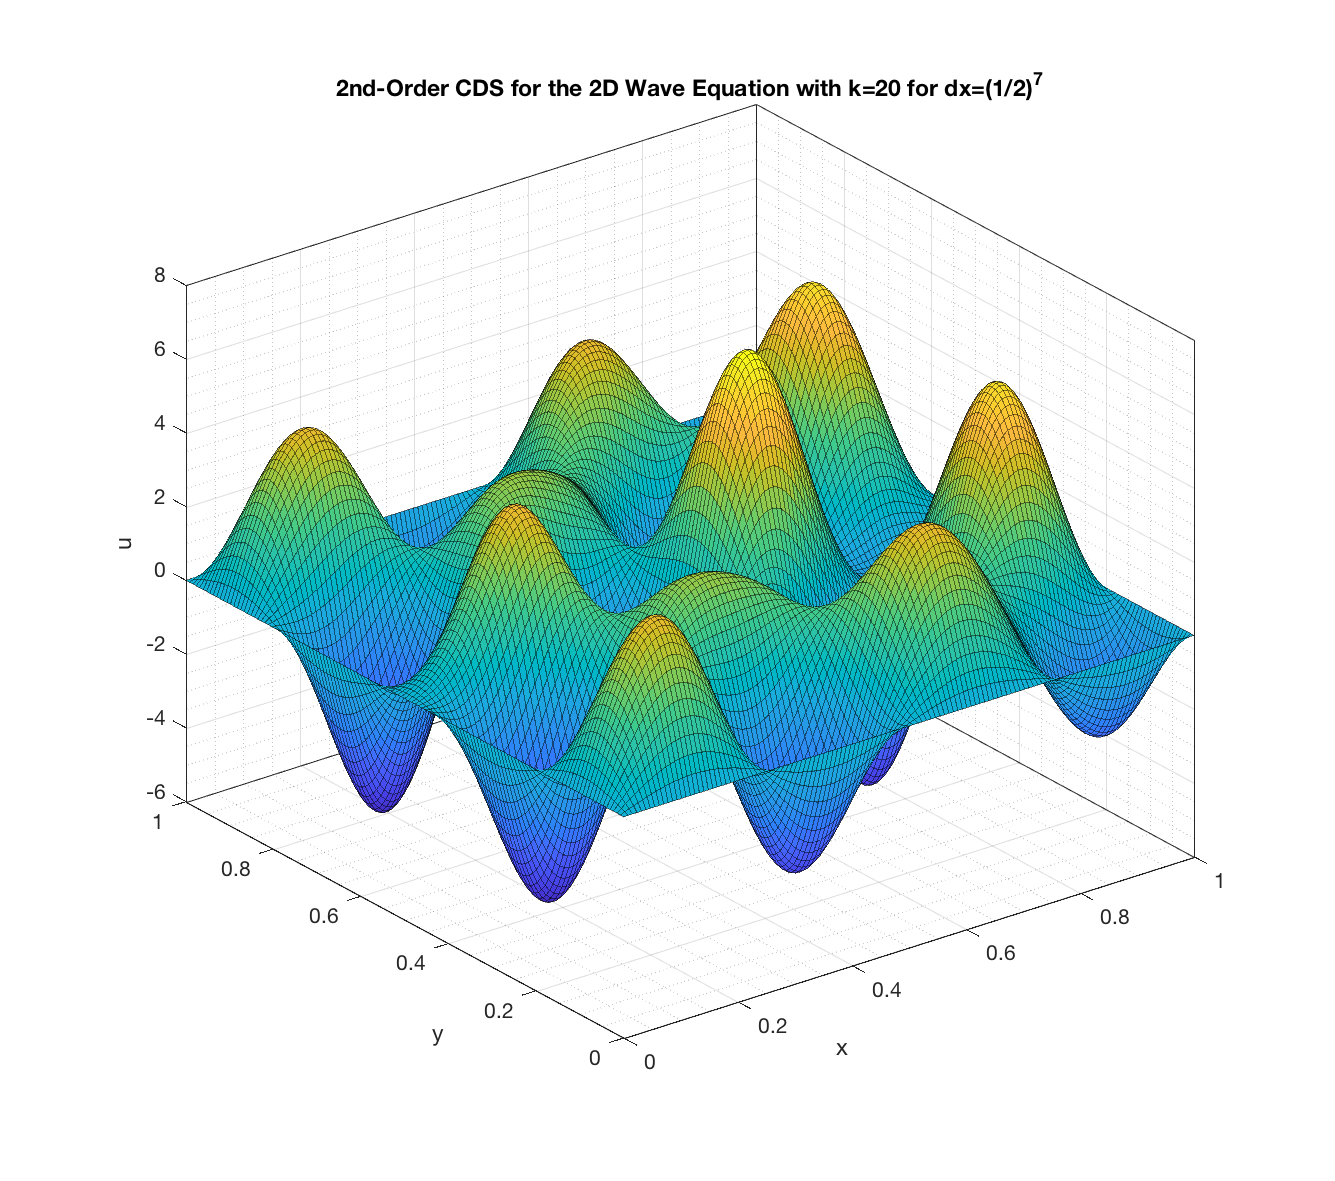
\includegraphics[width = 0.36\linewidth]{surface_plus_order_2_k_20_dx_order_7}
		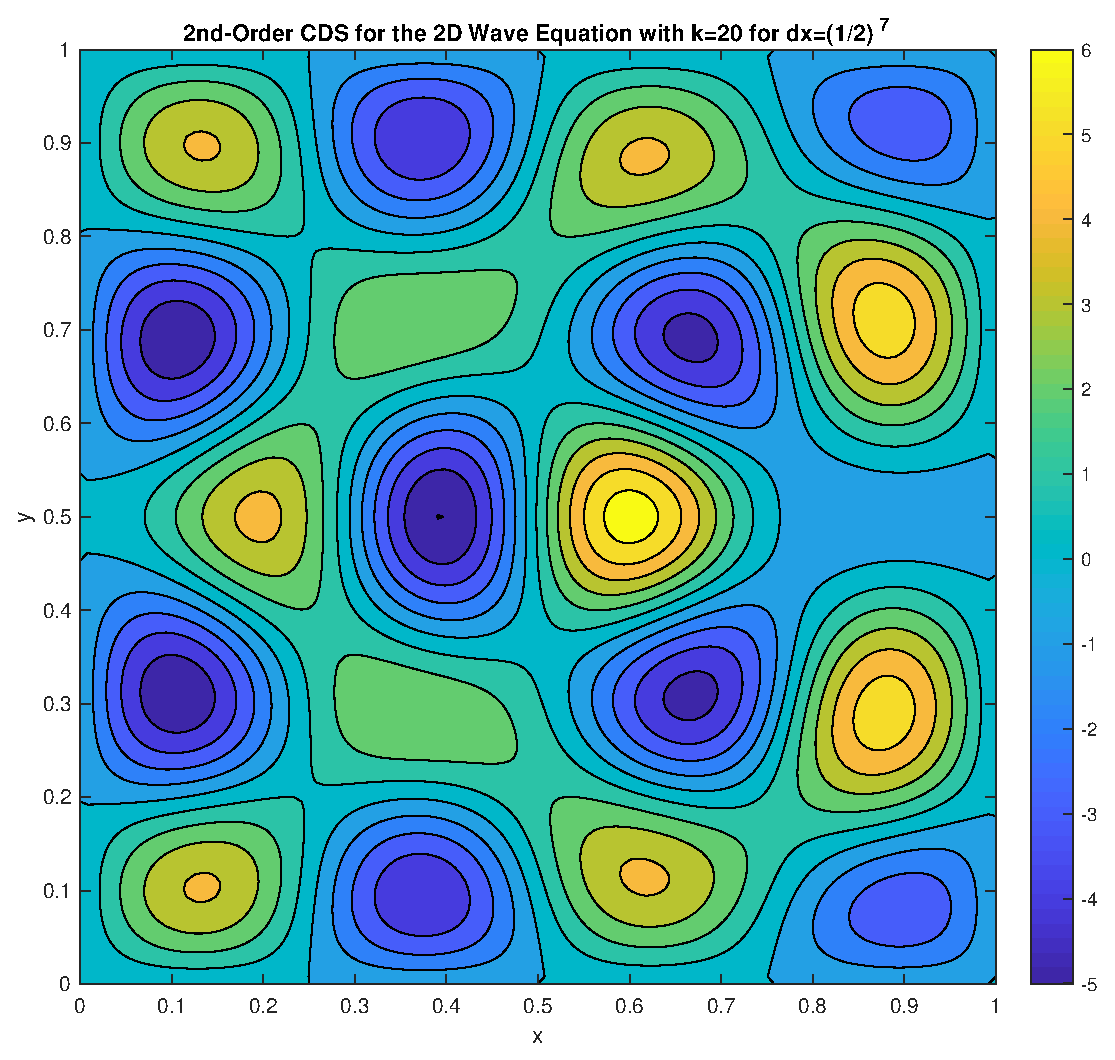
\includegraphics[width = 0.36\linewidth]{contour_plus_order_2_k_20_dx_order_7}
		\caption{2nd-Order CDS for the 2D Wave Equation with $k = 20$ for $\Delta x = (1/2)^7$}
	\end{center}
\end{figure}

\newpage

\subsubsection{4th-Order Central Difference Scheme - Wave Equation}

\begin{figure}[H]
	\begin{center}
		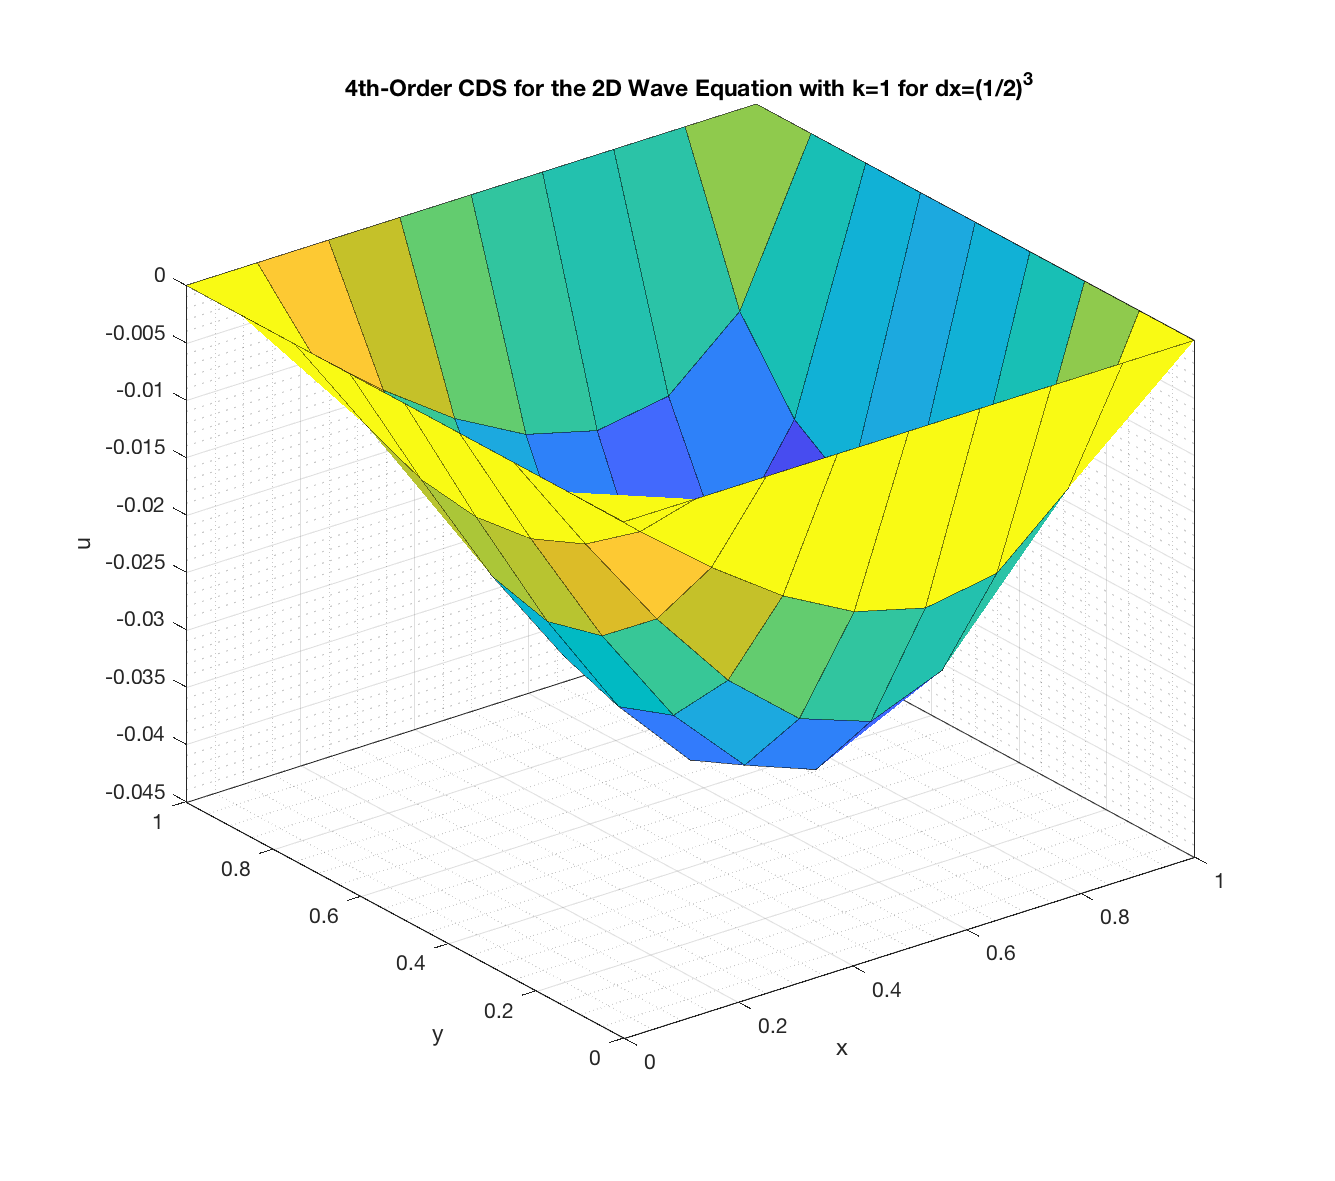
\includegraphics[width = 0.36\linewidth]{surface_plus_order_4_k_1_dx_order_3}
		\includegraphics[width = 0.36\linewidth]{contour_plus_order_4_k_1_dx_order_3}
		\caption{4th-Order CDS for the 2D Wave Equation with $k = 1$ for $\Delta x = (1/2)^3$}
	\end{center}
\end{figure}

\begin{figure}[H]
	\begin{center}
		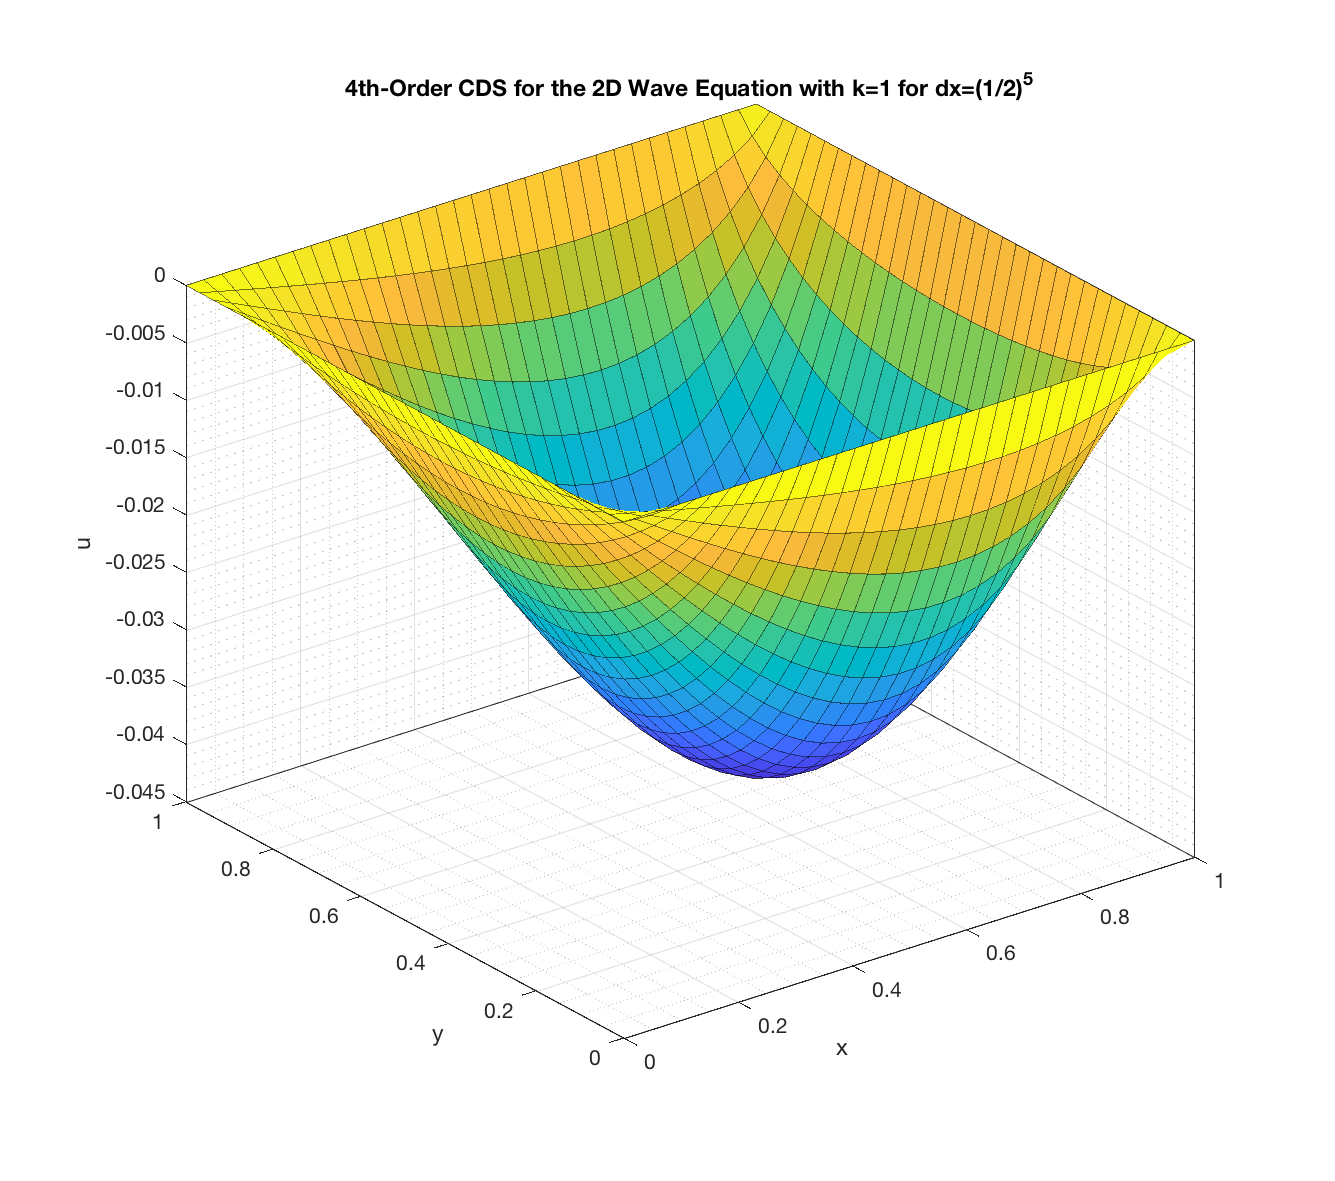
\includegraphics[width = 0.36\linewidth]{surface_plus_order_4_k_1_dx_order_5}
		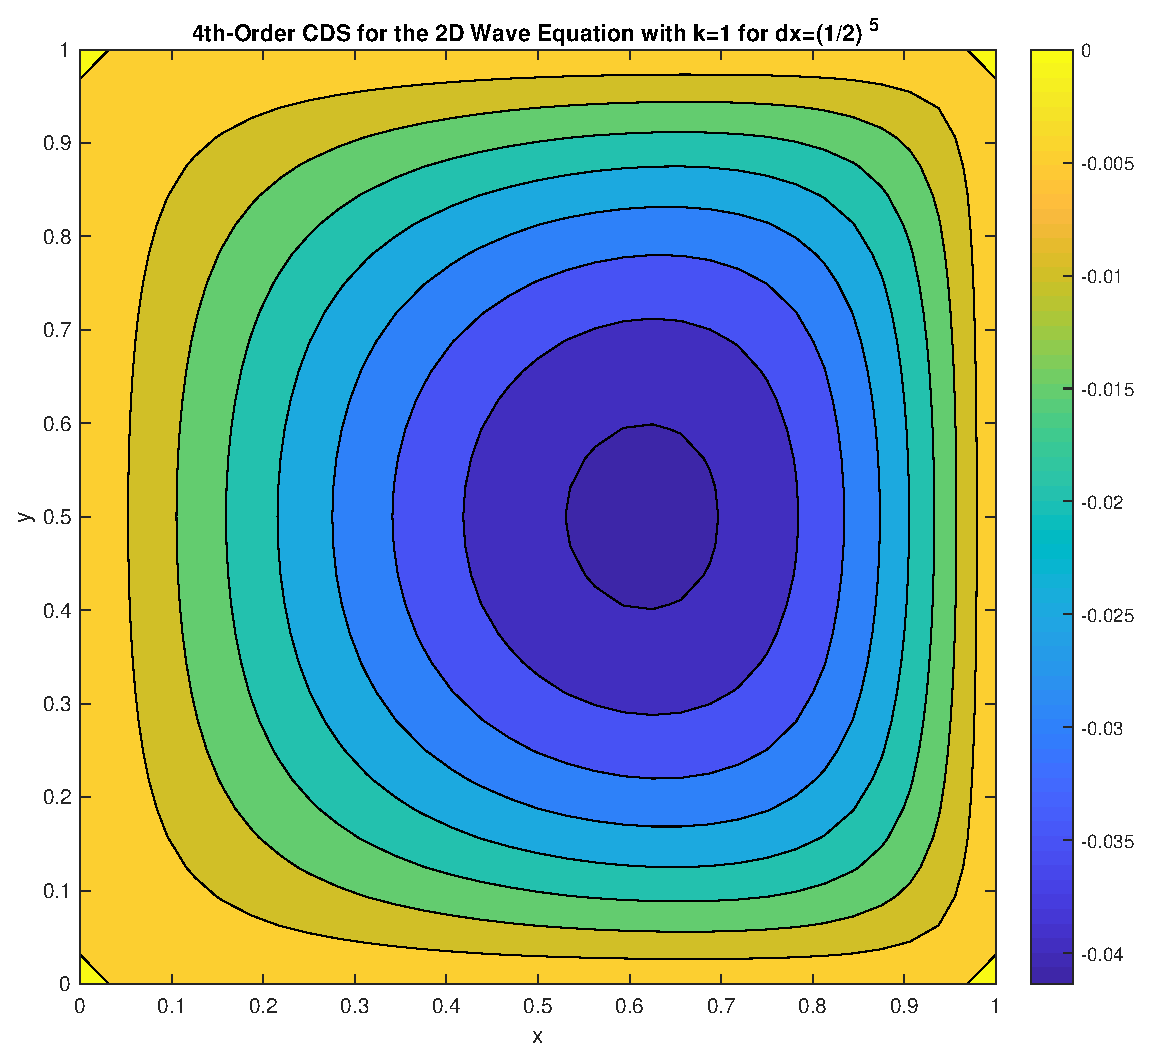
\includegraphics[width = 0.36\linewidth]{contour_plus_order_4_k_1_dx_order_5}
		\caption{4th-Order CDS for the 2D Wave Equation with $k = 1$ for $\Delta x = (1/2)^5$}
	\end{center}
\end{figure}

\begin{figure}[H]
	\begin{center}
		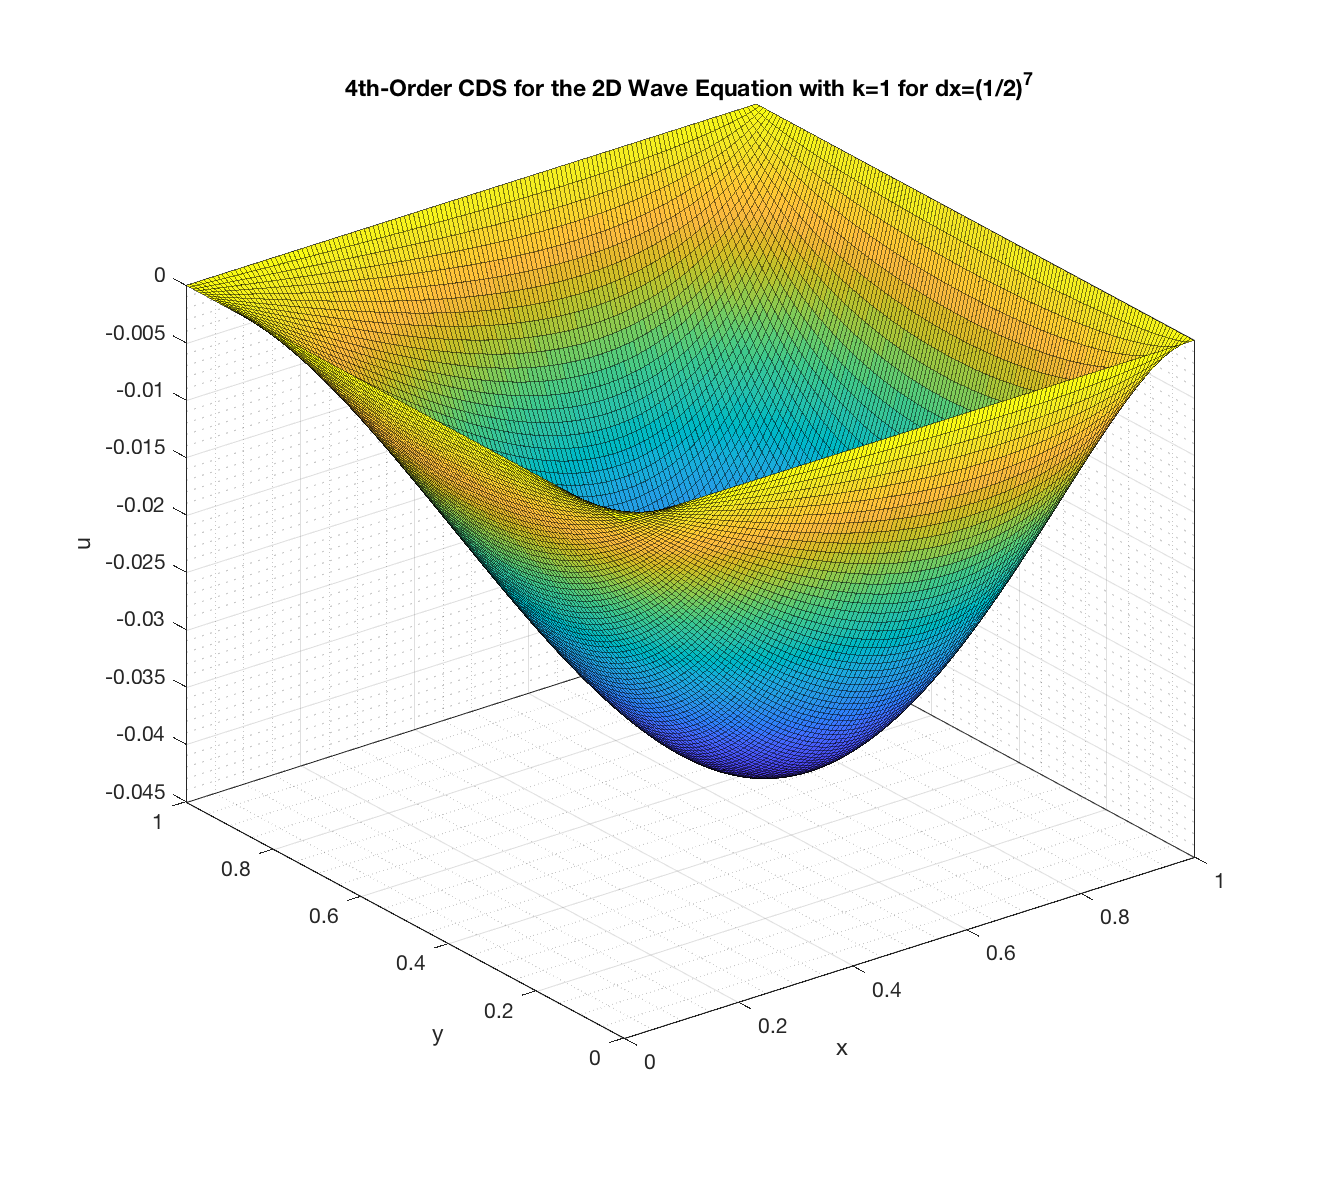
\includegraphics[width = 0.36\linewidth]{surface_plus_order_4_k_1_dx_order_7}
		\includegraphics[width = 0.36\linewidth]{contour_plus_order_4_k_1_dx_order_7}
		\caption{4th-Order CDS for the 2D Wave Equation with $k = 1$ for $\Delta x = (1/2)^7$}
	\end{center}
\end{figure}

\newpage

\begin{figure}[H]
	\begin{center}
		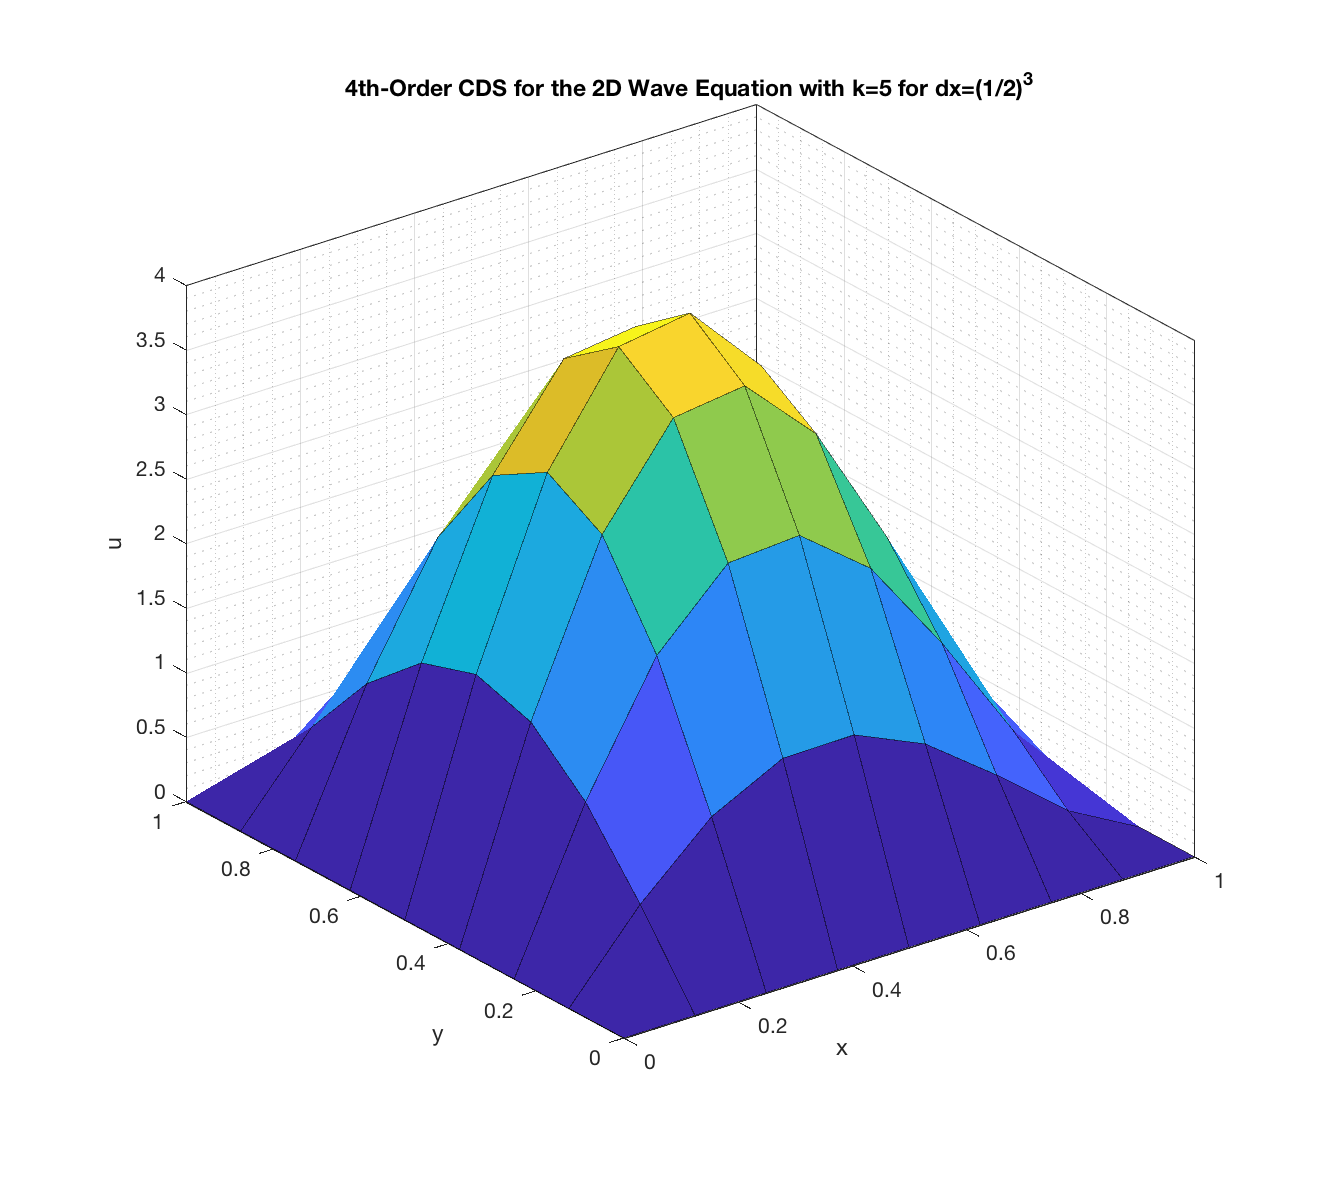
\includegraphics[width = 0.36\linewidth]{surface_plus_order_4_k_5_dx_order_3}
		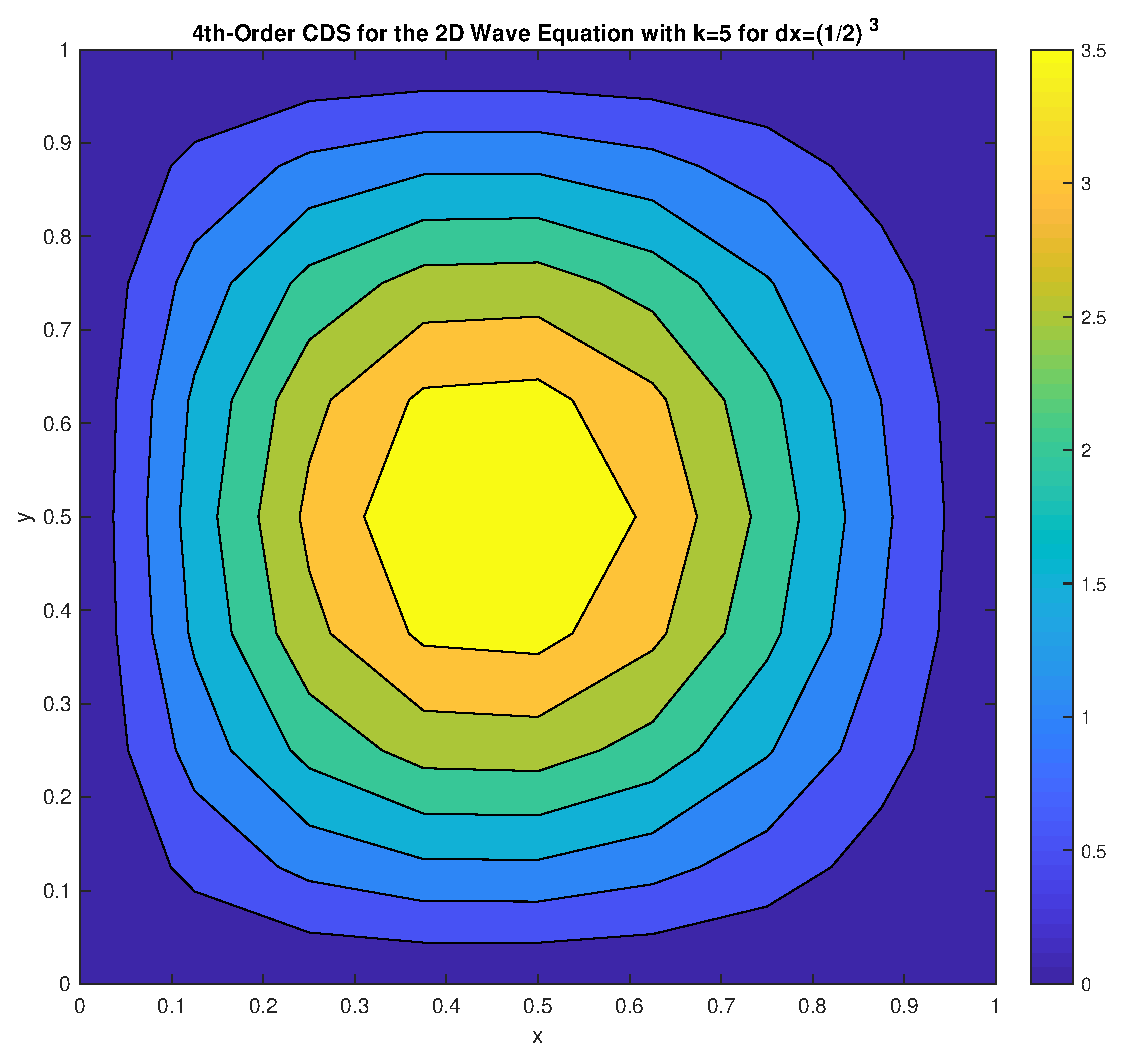
\includegraphics[width = 0.36\linewidth]{contour_plus_order_4_k_5_dx_order_3}
		\caption{4th-Order CDS for the 2D Wave Equation with $k = 5$ for $\Delta x = (1/2)^3$}
	\end{center}
\end{figure}

\begin{figure}[H]
	\begin{center}
		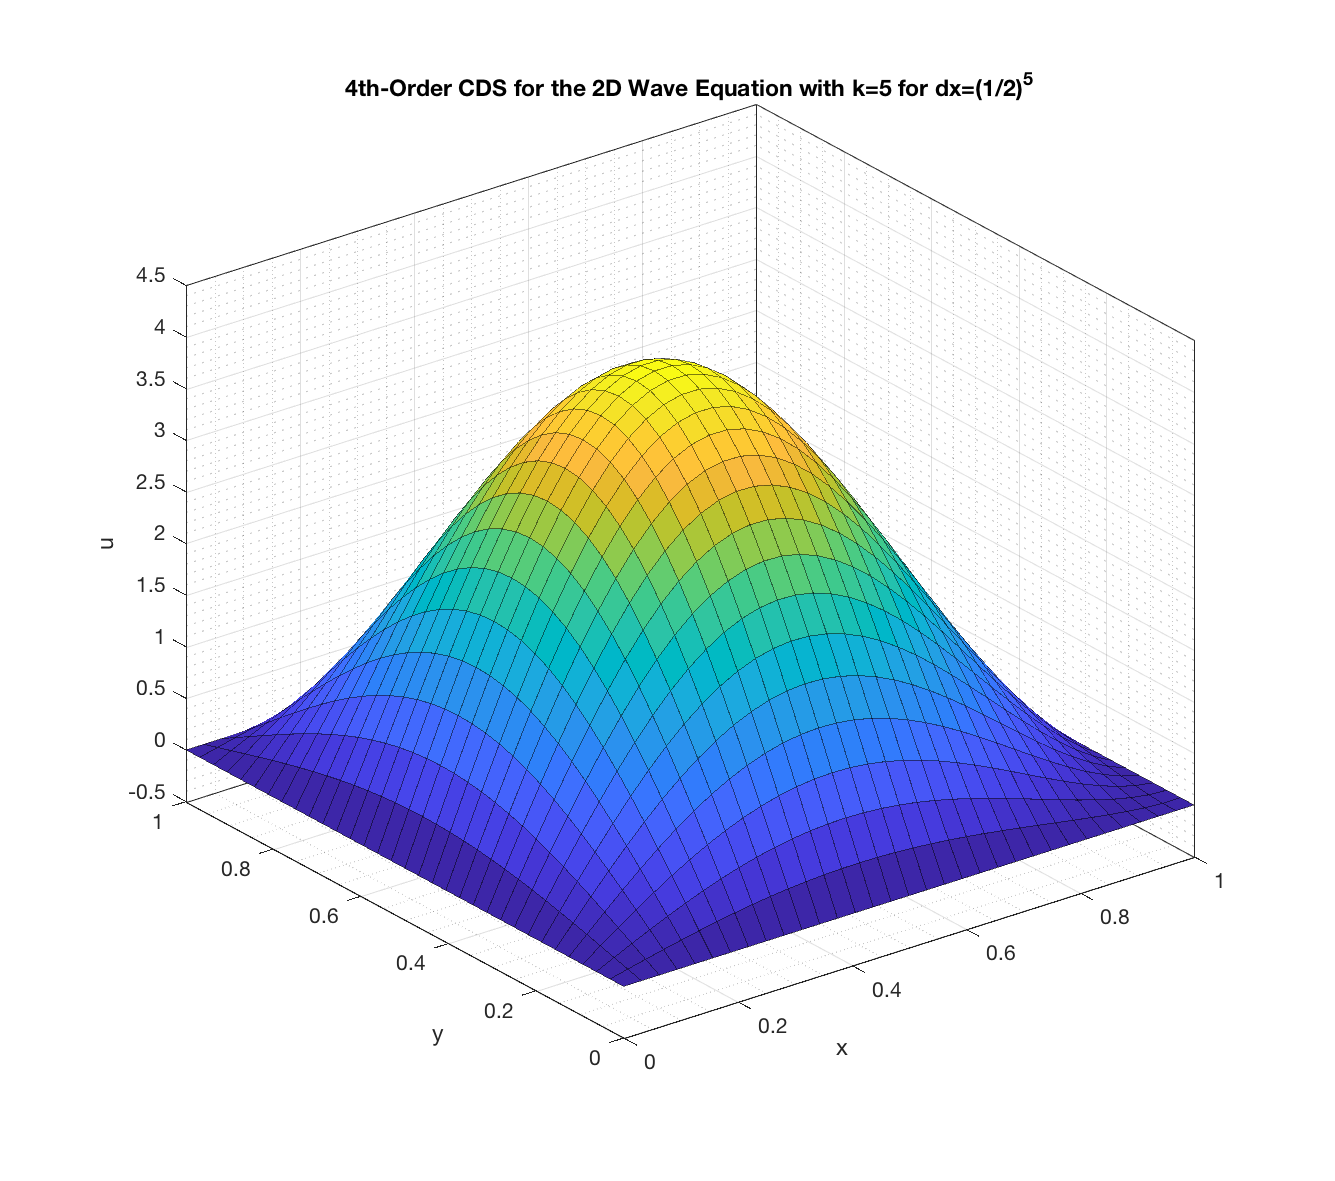
\includegraphics[width = 0.36\linewidth]{surface_plus_order_4_k_5_dx_order_5}
		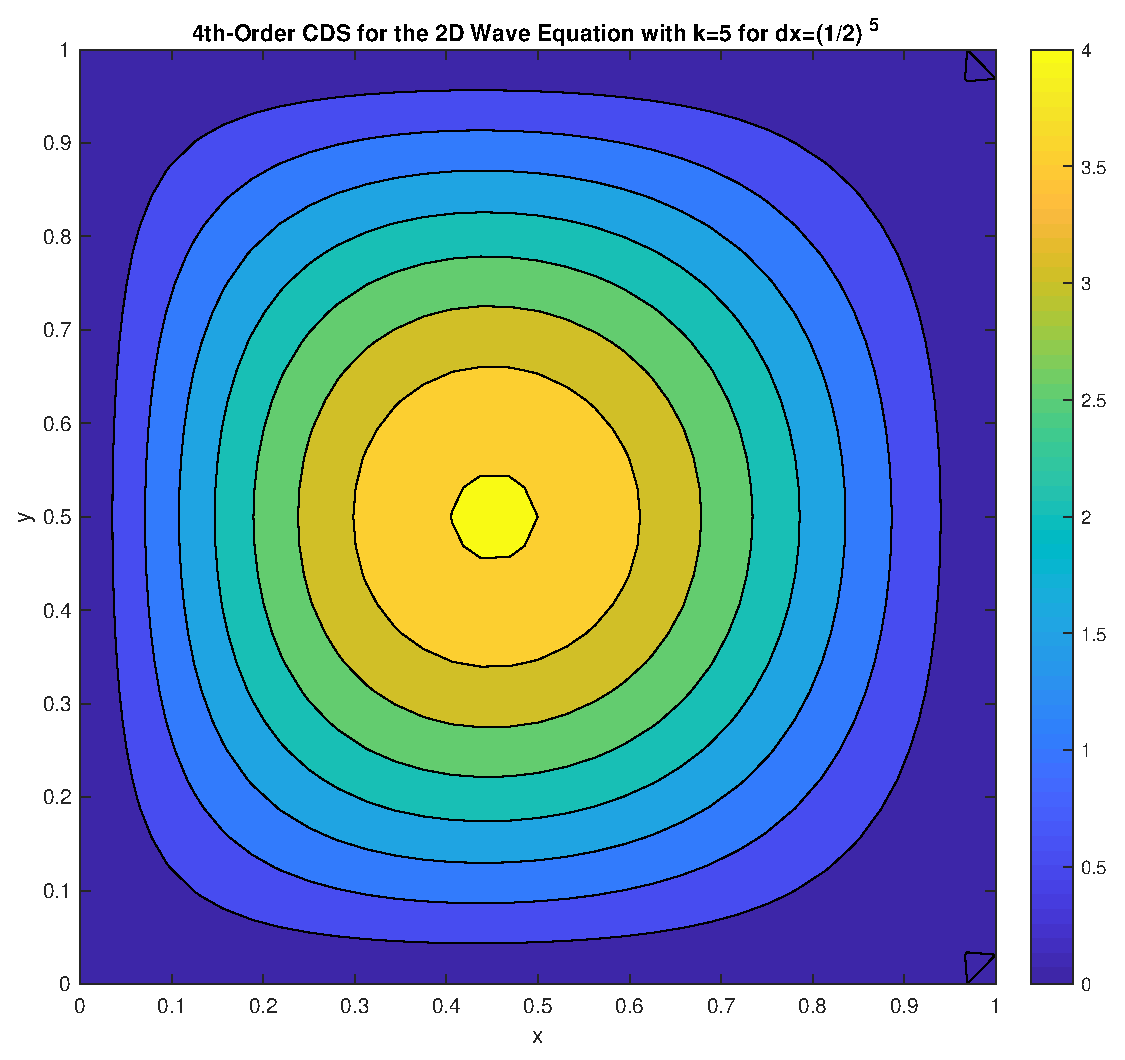
\includegraphics[width = 0.36\linewidth]{contour_plus_order_4_k_5_dx_order_5}
		\caption{4th-Order CDS for the 2D Wave Equation with $k = 5$ for $\Delta x = (1/2)^5$}
	\end{center}
\end{figure}

\begin{figure}[H]
	\begin{center}
		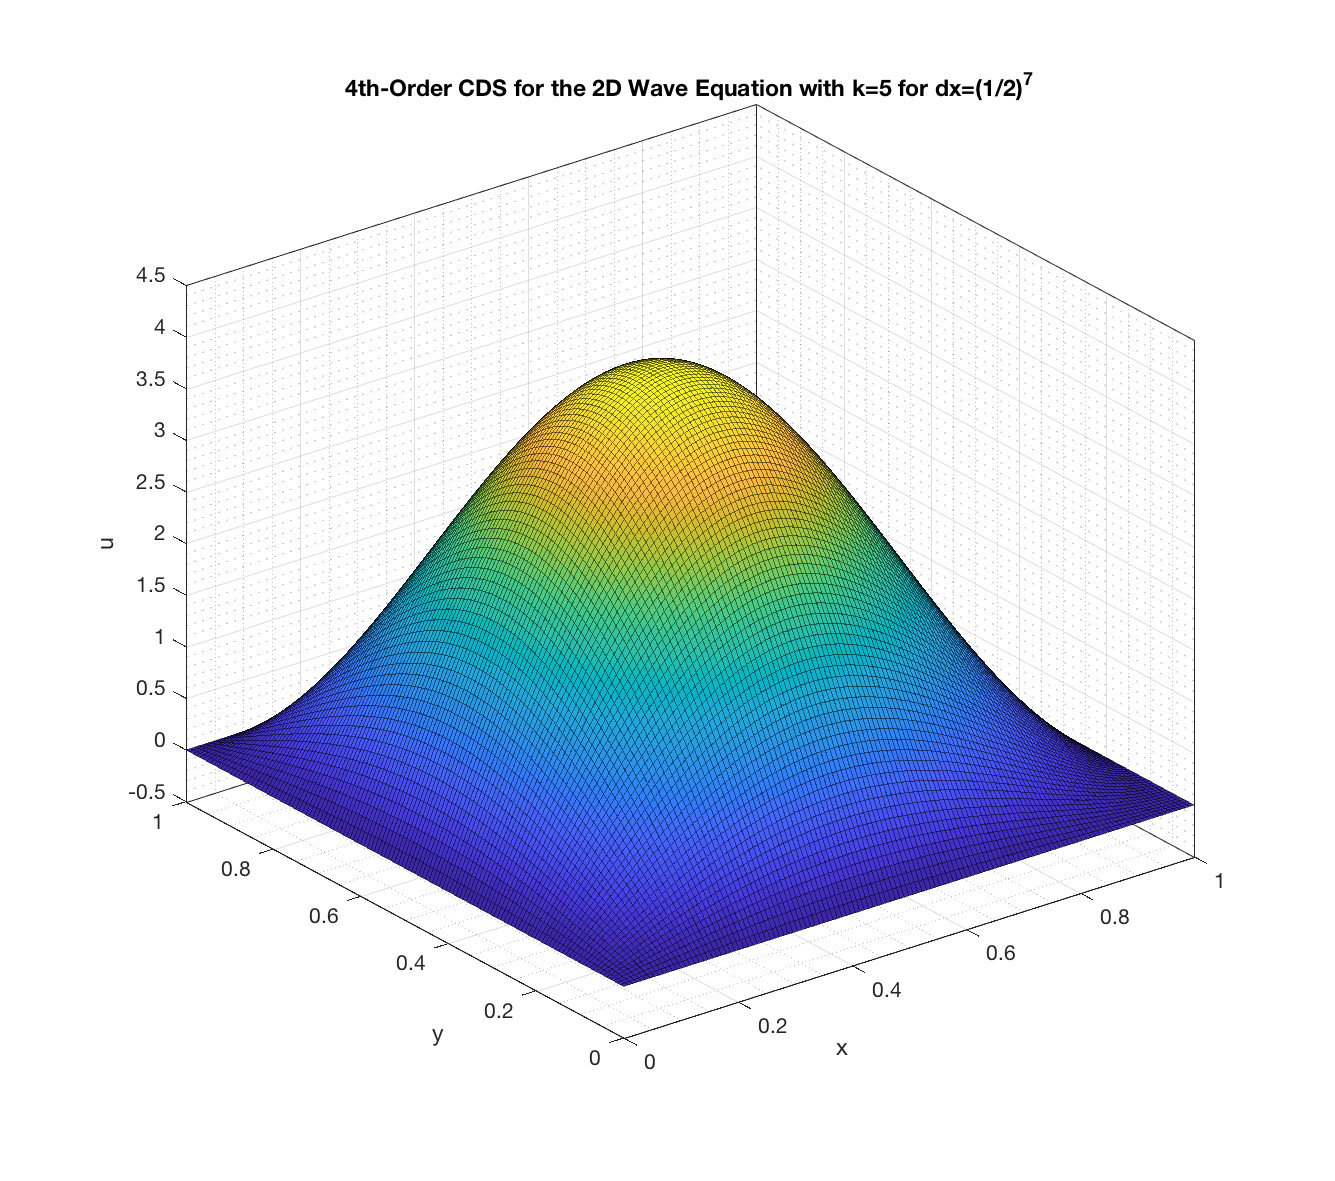
\includegraphics[width = 0.36\linewidth]{surface_plus_order_4_k_5_dx_order_7}
		\includegraphics[width = 0.36\linewidth]{contour_plus_order_4_k_5_dx_order_7}
		\caption{4th-Order CDS for the 2D Wave Equation with $k = 5$ for $\Delta x = (1/2)^7$}
	\end{center}
\end{figure}

\newpage

\begin{figure}[H]
	\begin{center}
		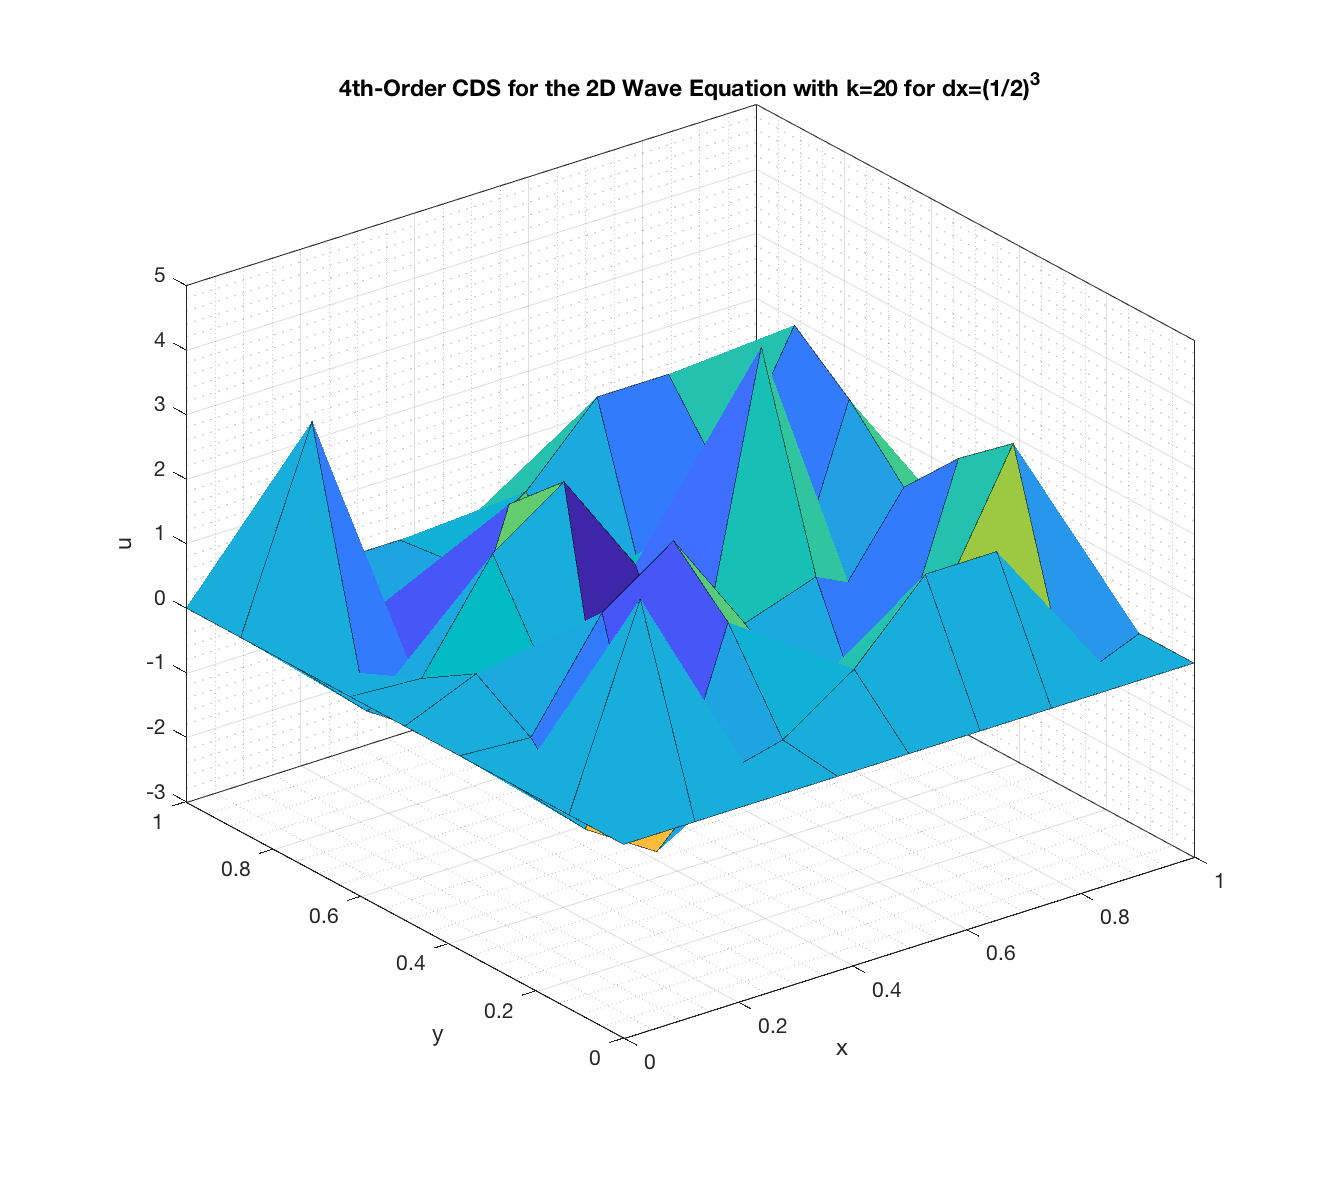
\includegraphics[width = 0.36\linewidth]{surface_plus_order_4_k_20_dx_order_3}
		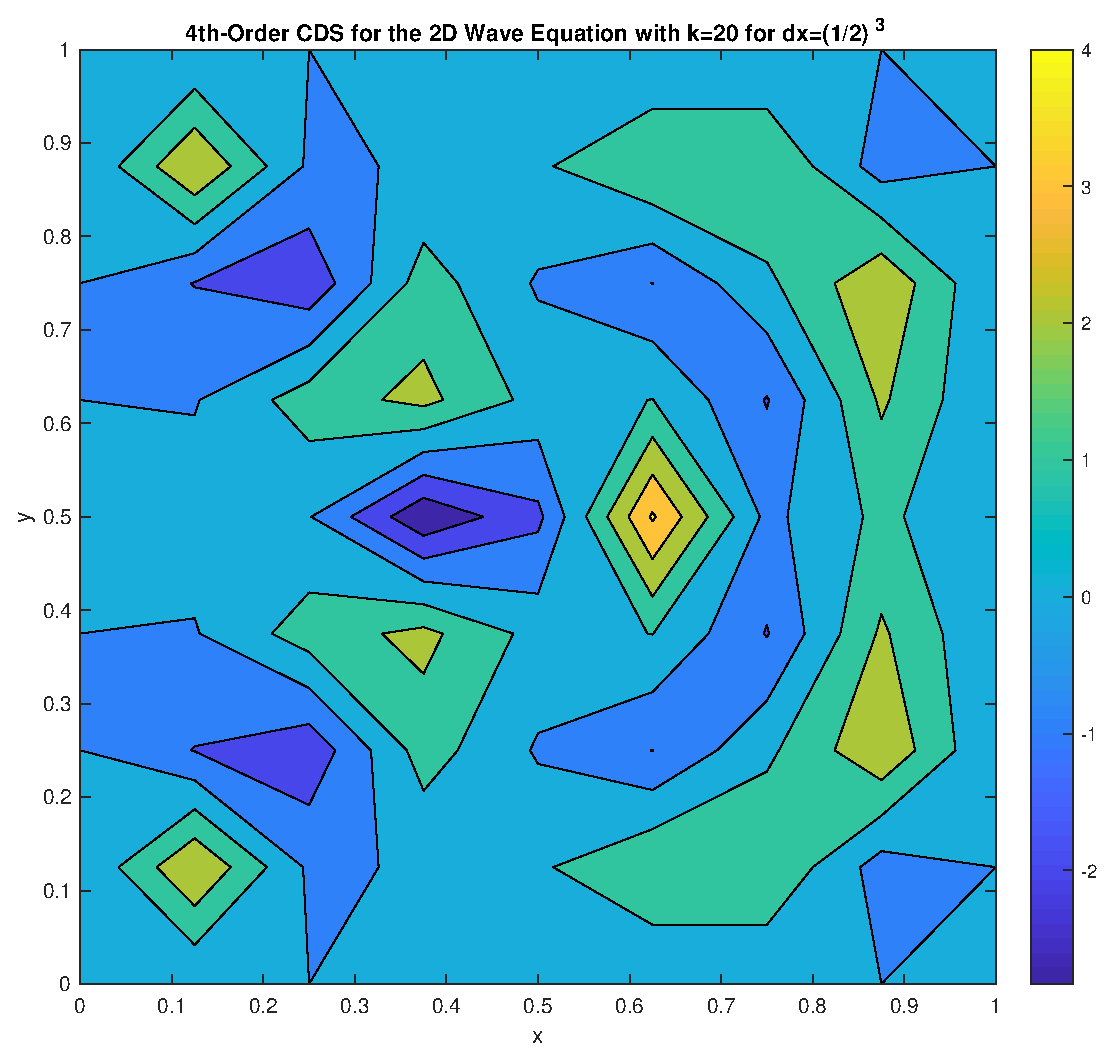
\includegraphics[width = 0.36\linewidth]{contour_plus_order_4_k_20_dx_order_3}
		\caption{4th-Order CDS for the 2D Wave Equation with $k = 20$ for $\Delta x = (1/2)^3$}
	\end{center}
\end{figure}

\begin{figure}[H]
	\begin{center}
		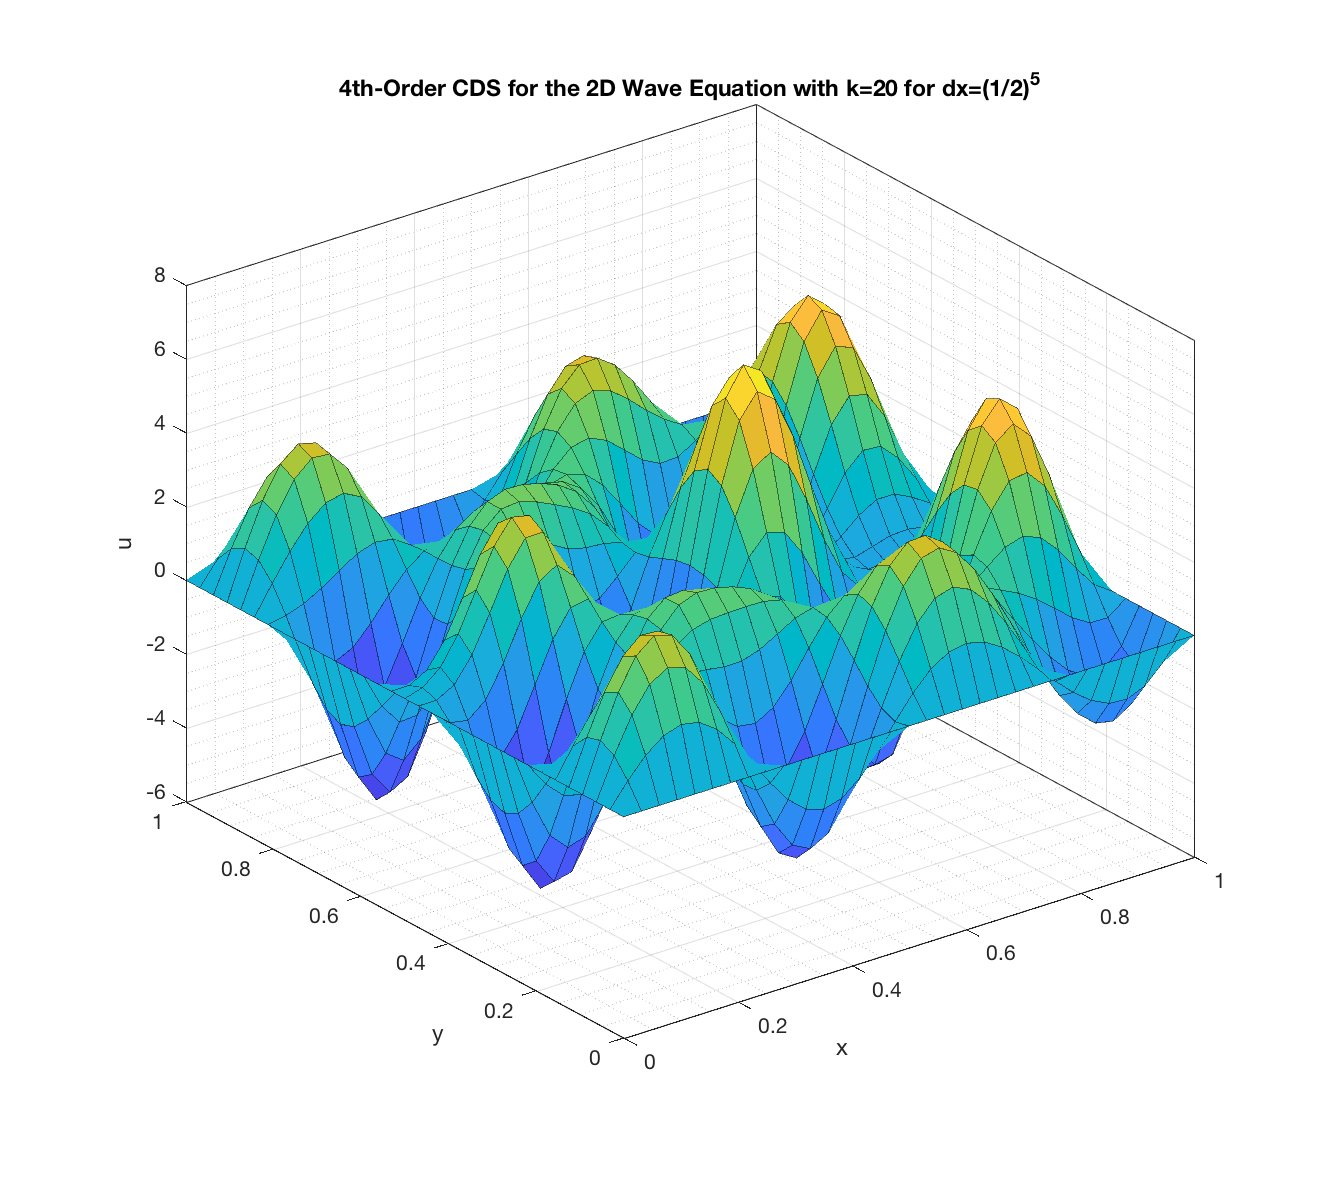
\includegraphics[width = 0.36\linewidth]{surface_plus_order_4_k_20_dx_order_5}
		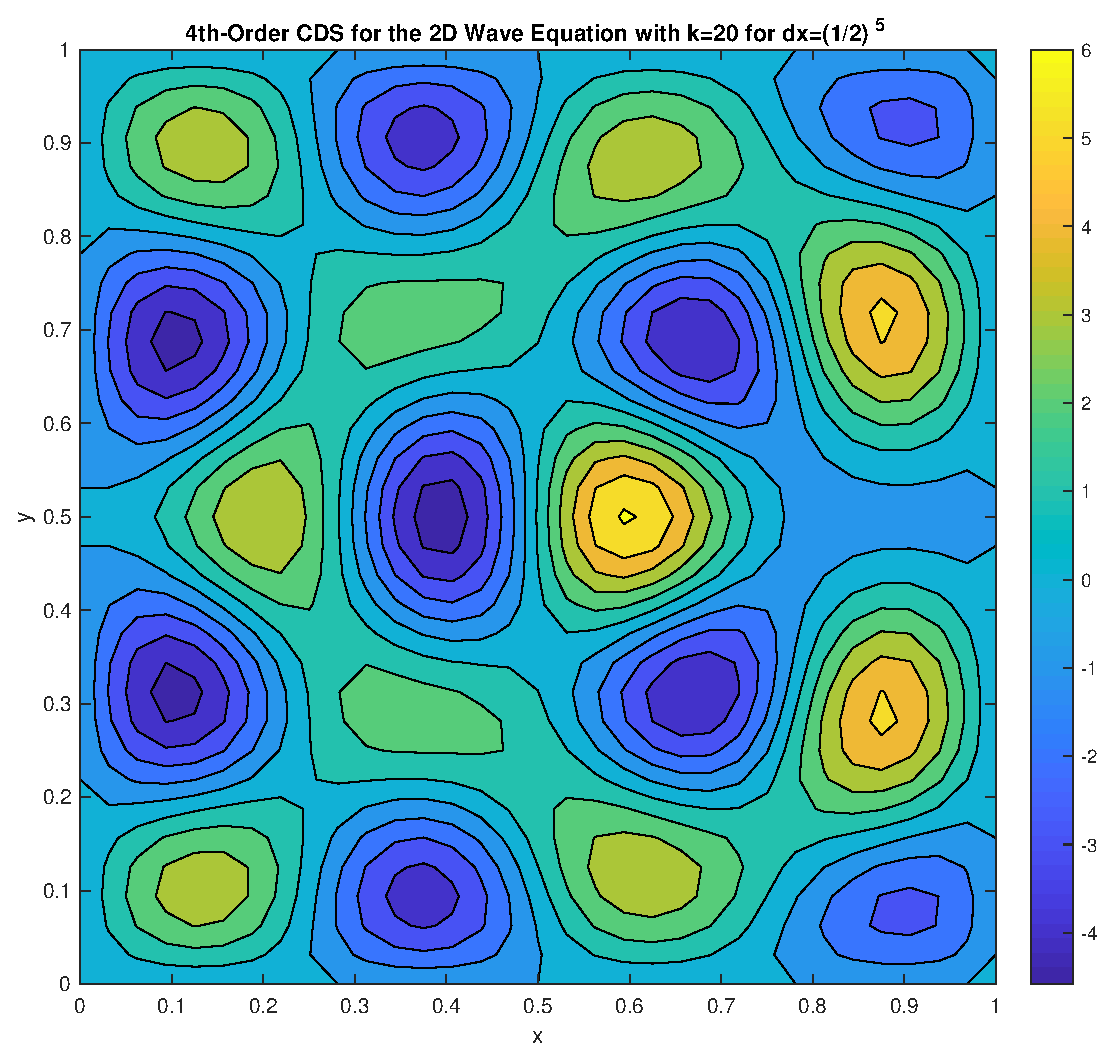
\includegraphics[width = 0.36\linewidth]{contour_plus_order_4_k_20_dx_order_5}
		\caption{4th-Order CDS for the 2D Wave Equation with $k = 20$ for $\Delta x = (1/2)^5$}
	\end{center}
\end{figure}

\begin{figure}[H]
	\begin{center}
		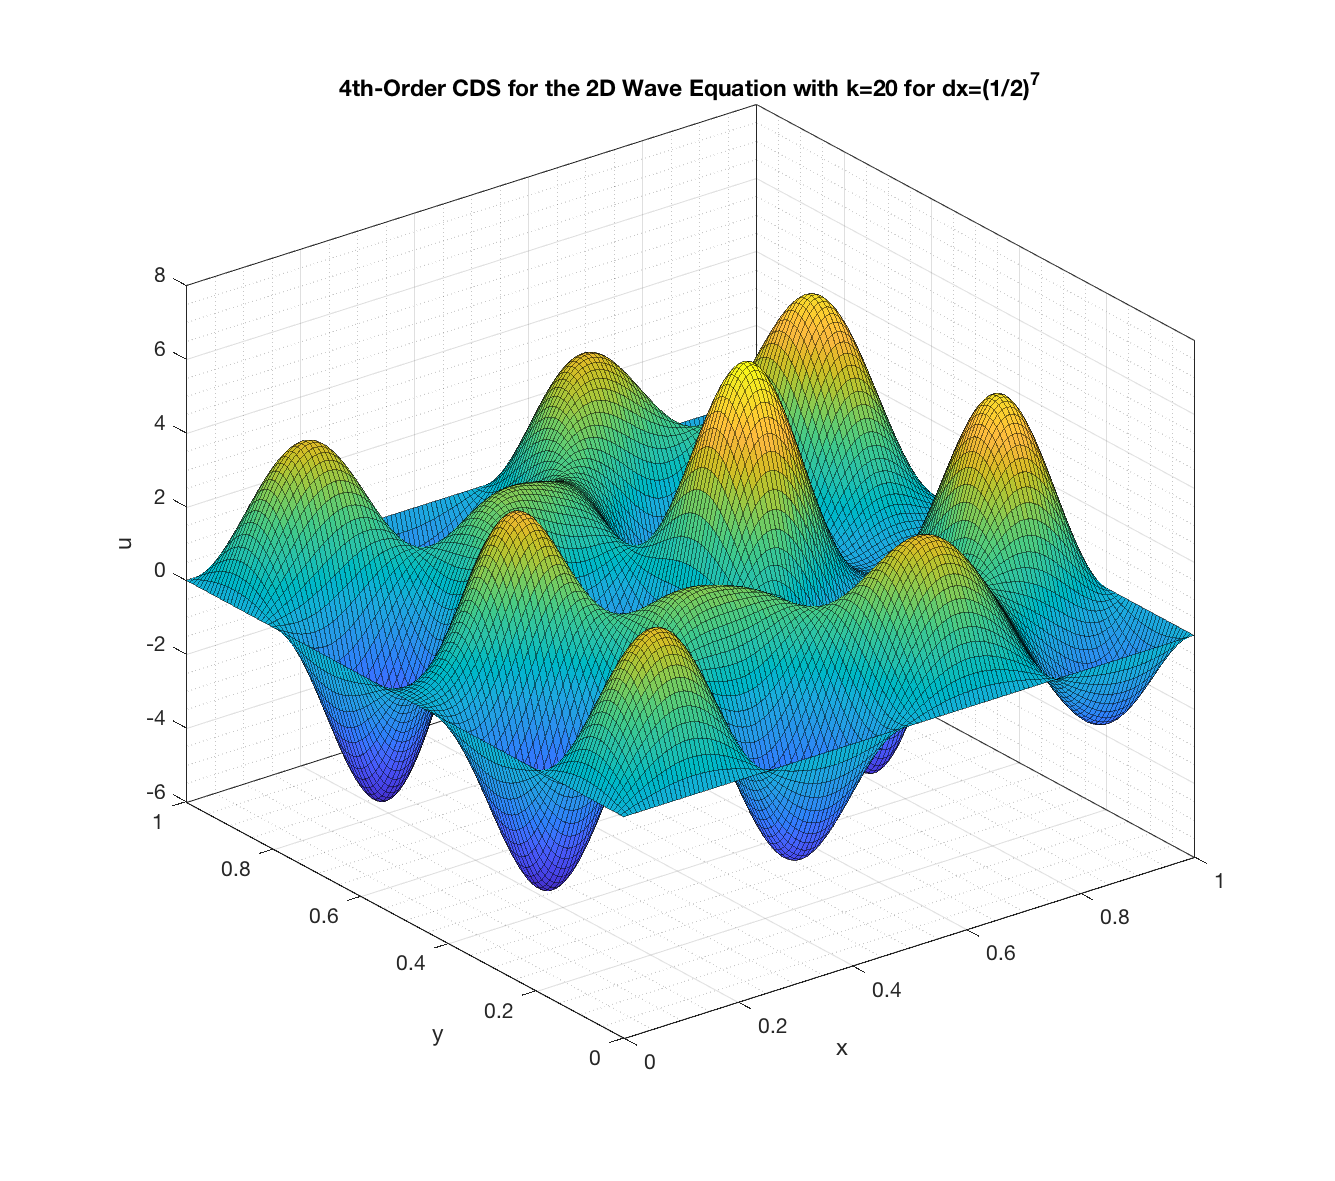
\includegraphics[width = 0.36\linewidth]{surface_plus_order_4_k_20_dx_order_7}
		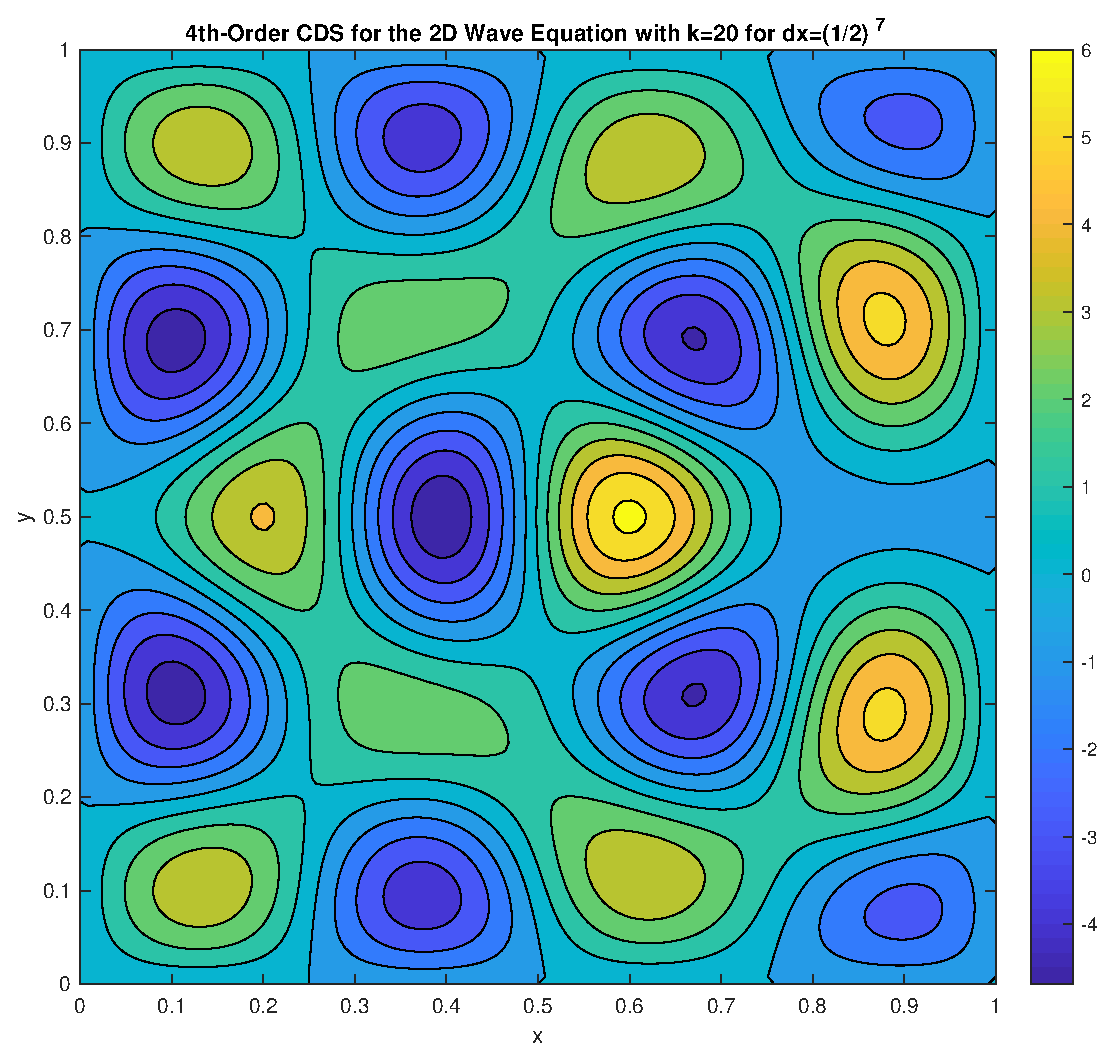
\includegraphics[width = 0.36\linewidth]{contour_plus_order_4_k_20_dx_order_7}
		\caption{4th-Order CDS for the 2D Wave Equation with $k = 20$ for $\Delta x = (1/2)^7$}
	\end{center}
\end{figure}

\newpage

\subsubsection{2nd-Order Central Difference Scheme - Diffusion Equation}

\begin{figure}[H]
	\begin{center}
		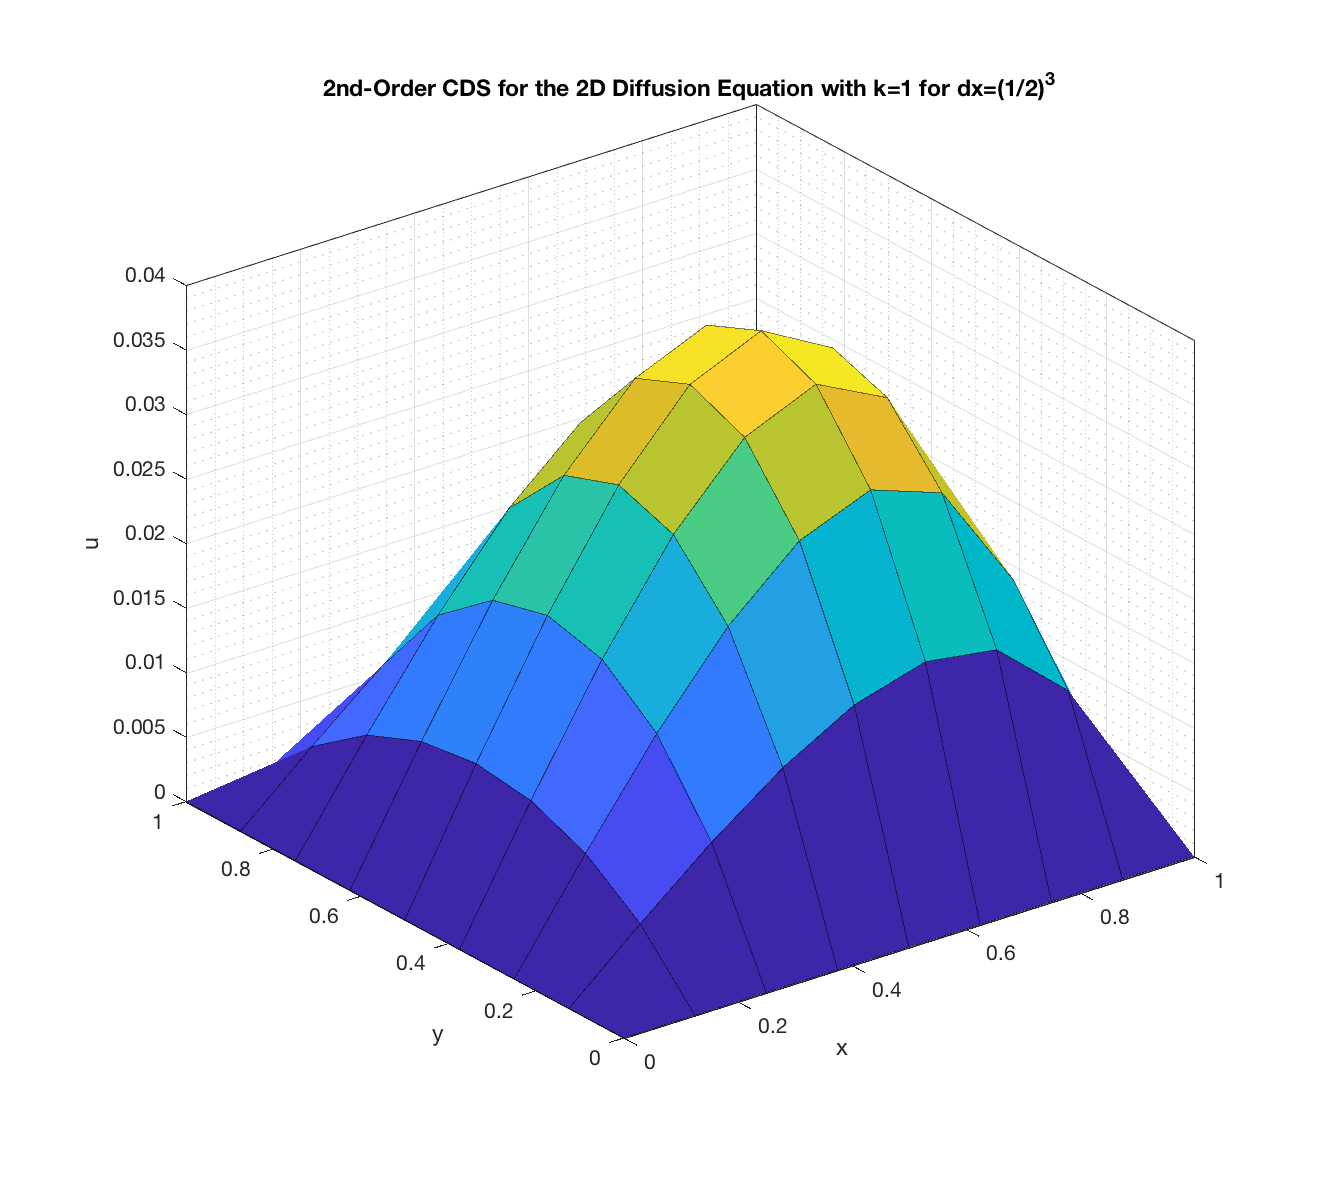
\includegraphics[width = 0.36\linewidth]{surface_minus_order_2_k_1_dx_order_3}
		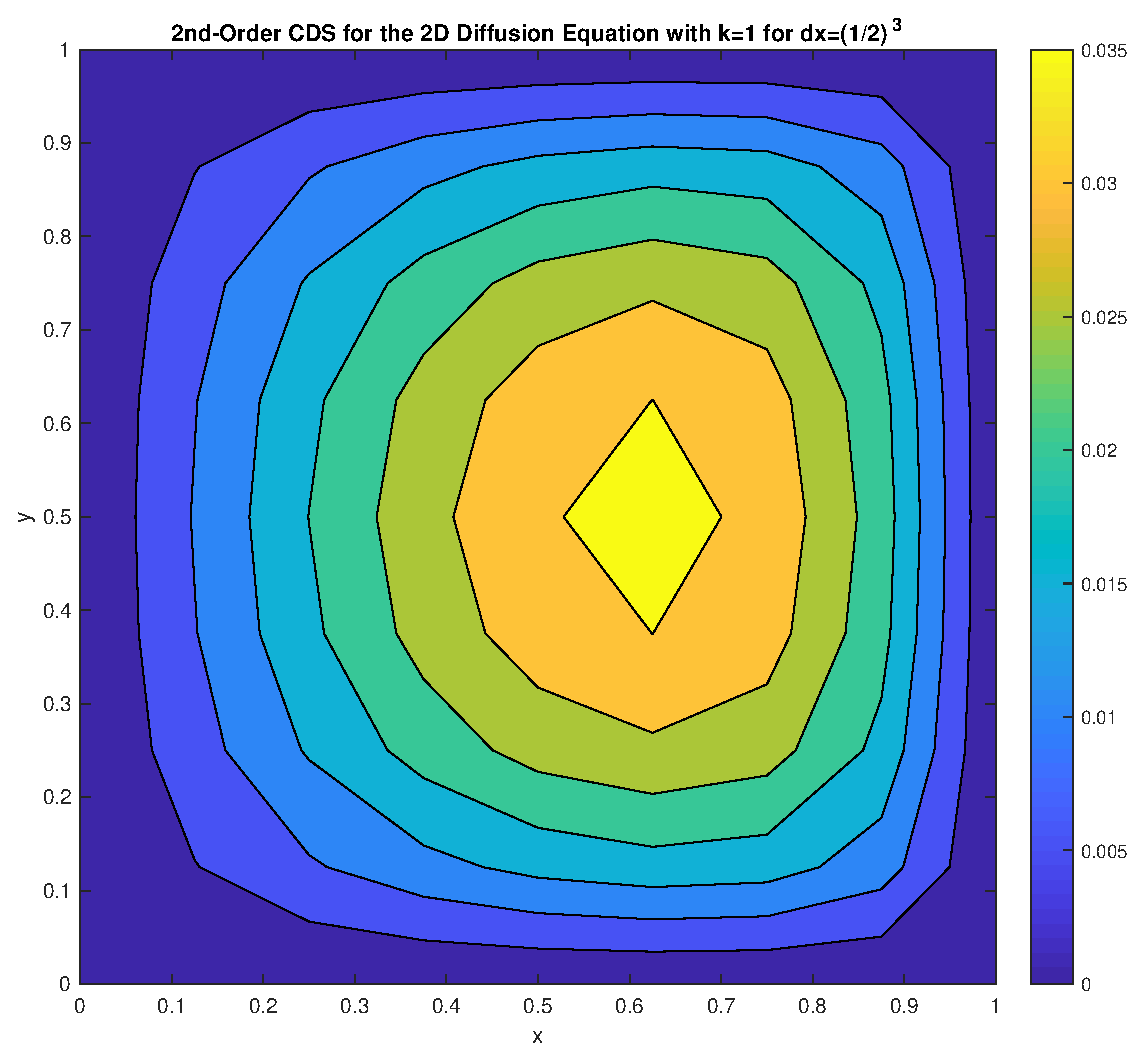
\includegraphics[width = 0.36\linewidth]{contour_minus_order_2_k_1_dx_order_3}
		\caption{2nd-Order CDS for the 2D Diffusion Equation with $k = 1$ for $\Delta x = (1/2)^3$}
	\end{center}
\end{figure}

\begin{figure}[H]
	\begin{center}
		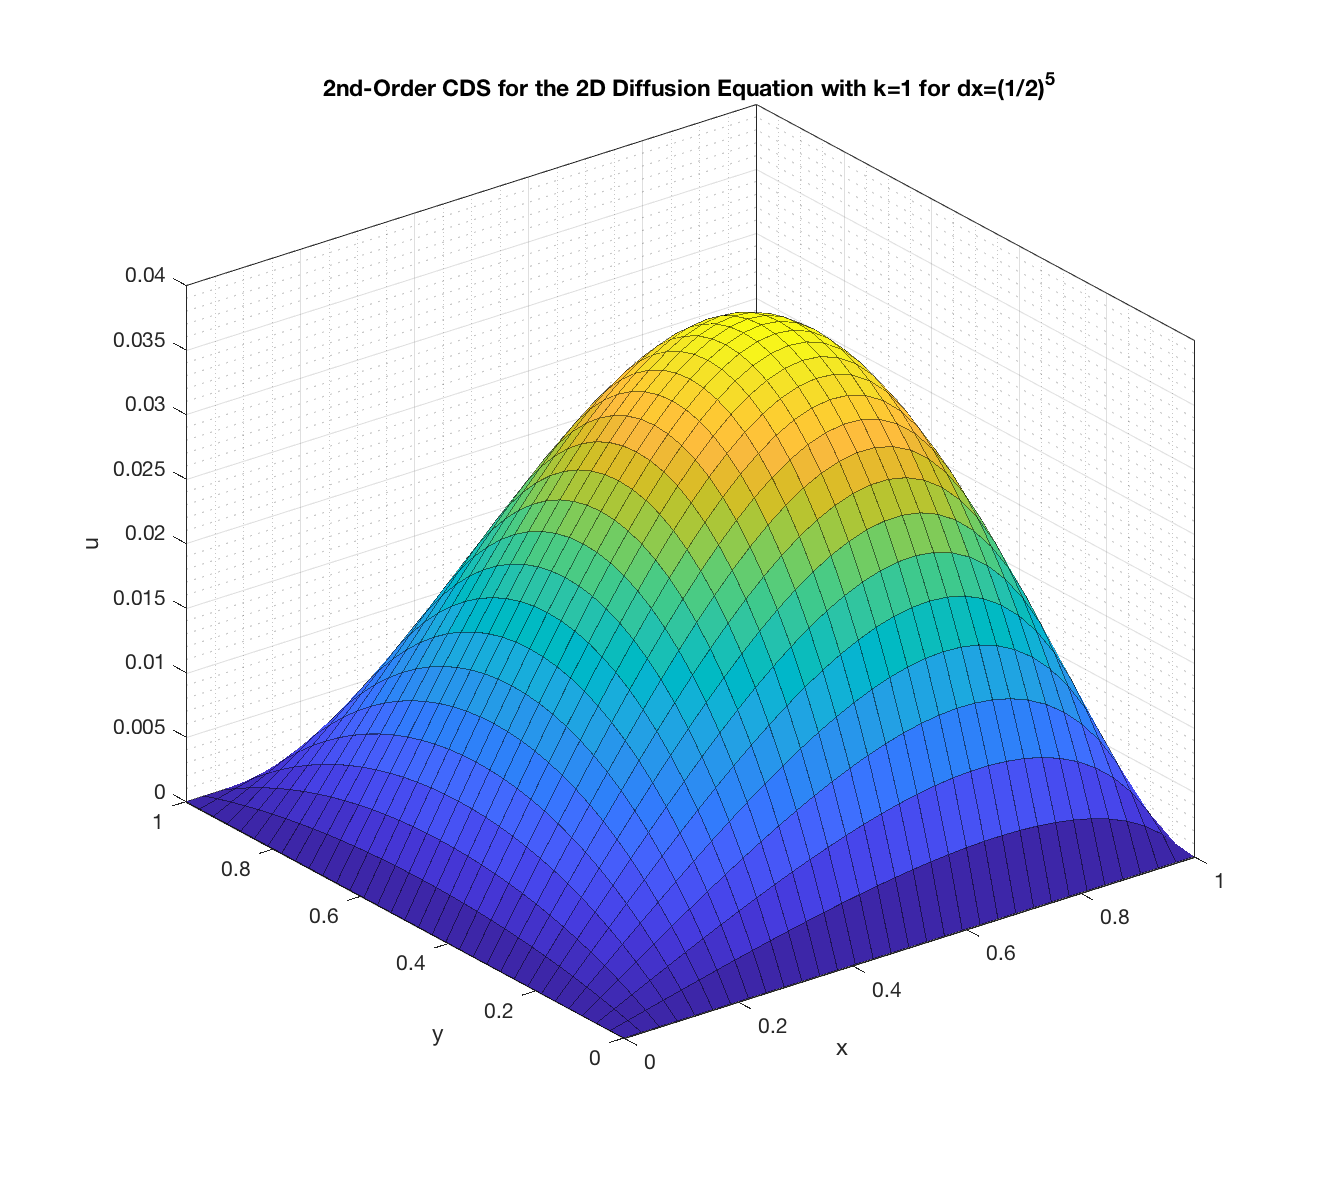
\includegraphics[width = 0.36\linewidth]{surface_minus_order_2_k_1_dx_order_5}
		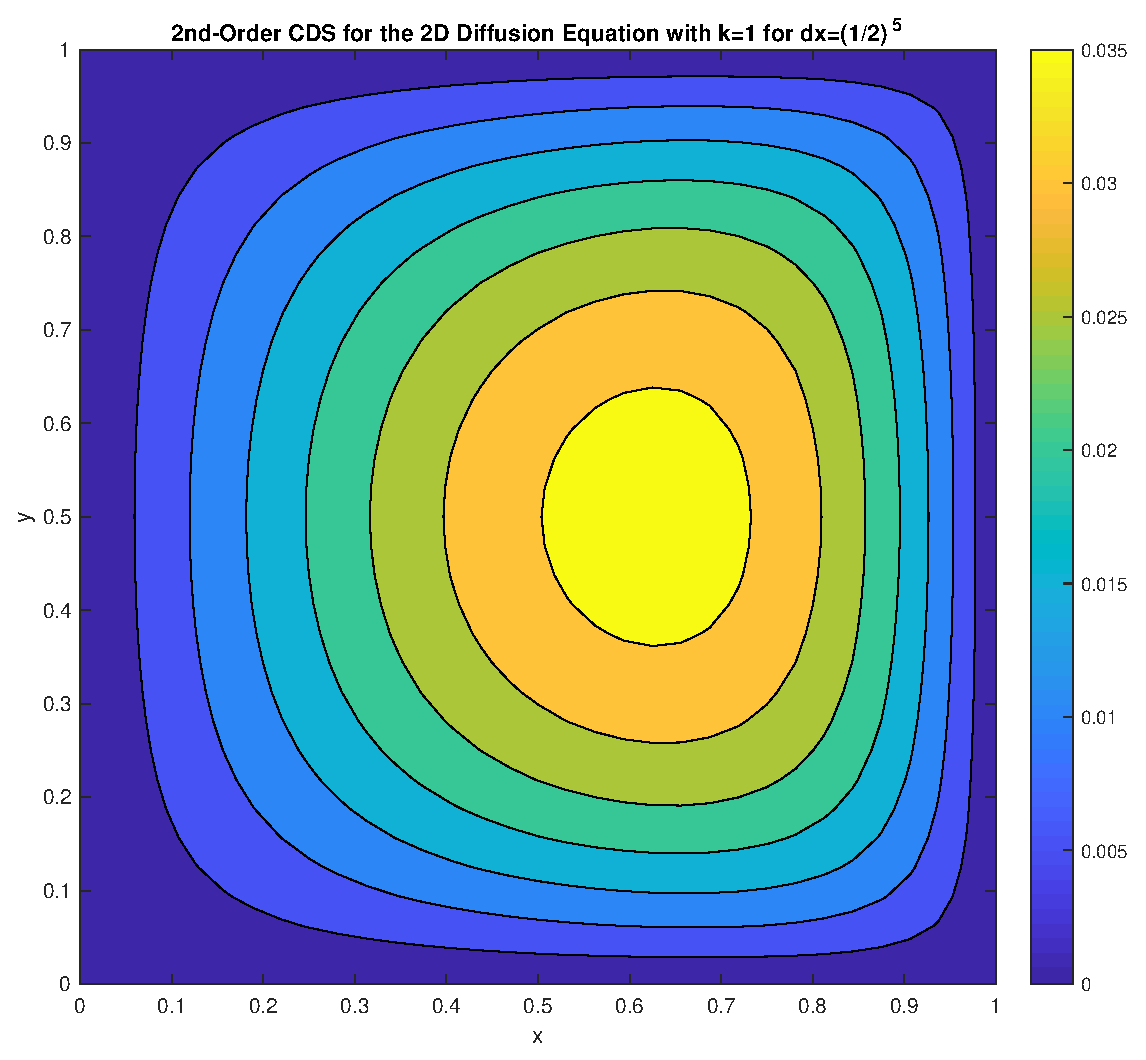
\includegraphics[width = 0.36\linewidth]{contour_minus_order_2_k_1_dx_order_5}
		\caption{2nd-Order CDS for the 2D Diffusion Equation with $k = 1$ for $\Delta x = (1/2)^5$}
	\end{center}
\end{figure}

\begin{figure}[H]
	\begin{center}
		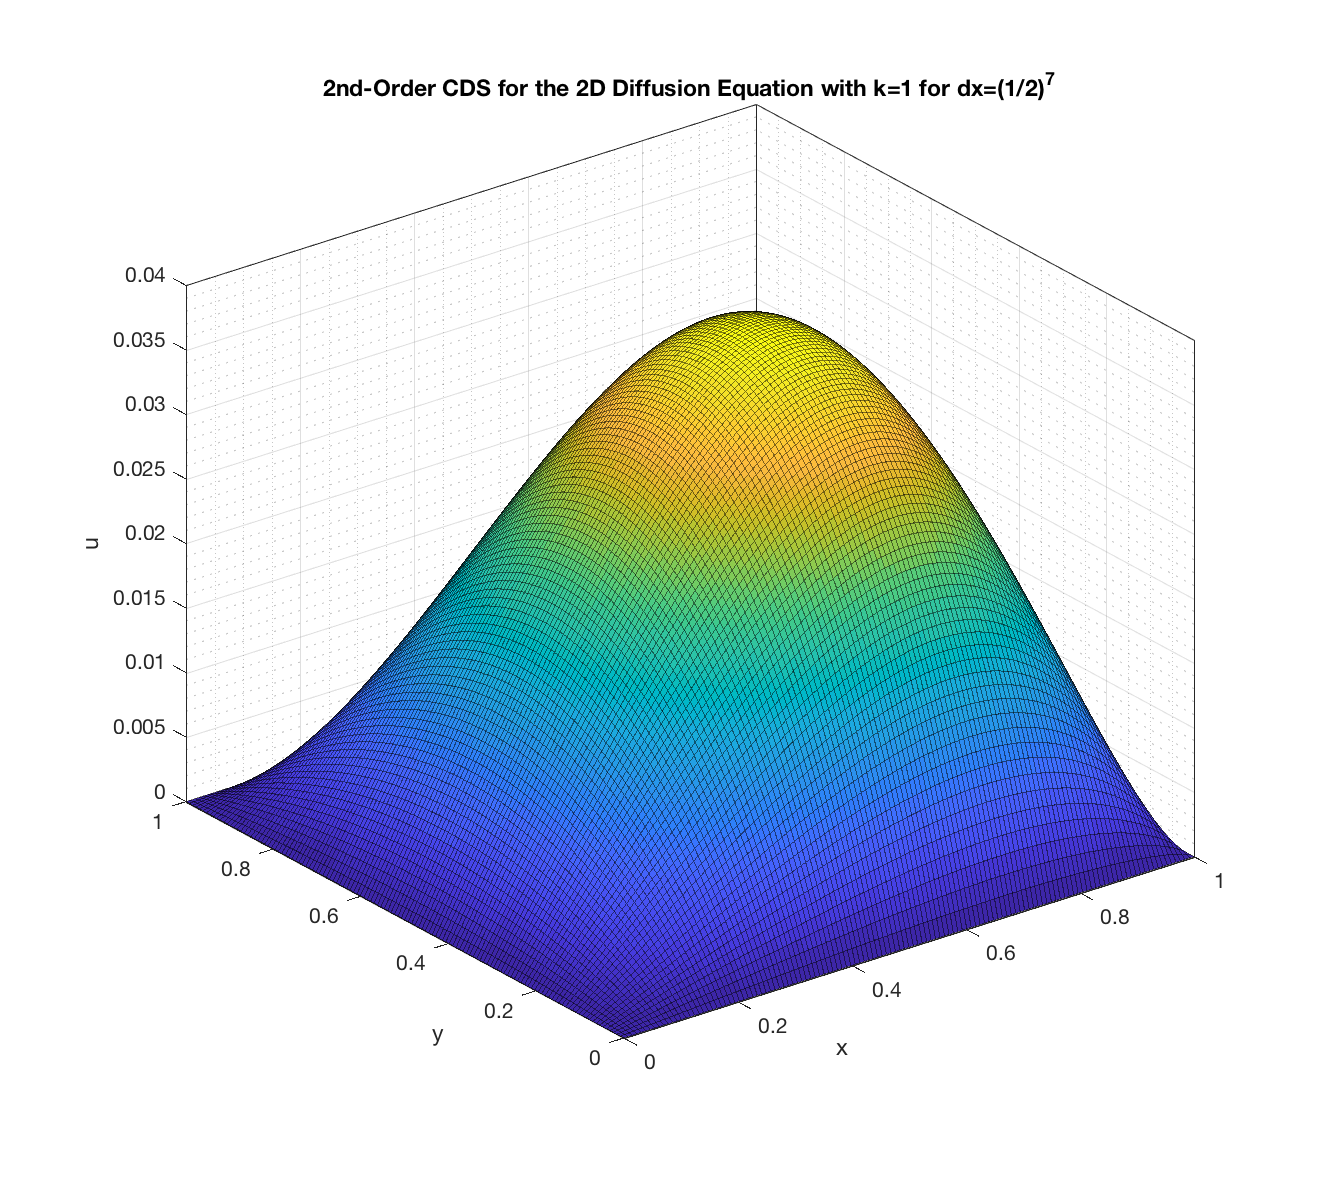
\includegraphics[width = 0.36\linewidth]{surface_minus_order_2_k_1_dx_order_7}
		\includegraphics[width = 0.36\linewidth]{contour_minus_order_2_k_1_dx_order_7}
		\caption{2nd-Order CDS for the 2D Diffusion Equation with $k = 1$ for $\Delta x = (1/2)^7$}
	\end{center}
\end{figure}

\newpage

\begin{figure}[H]
	\begin{center}
		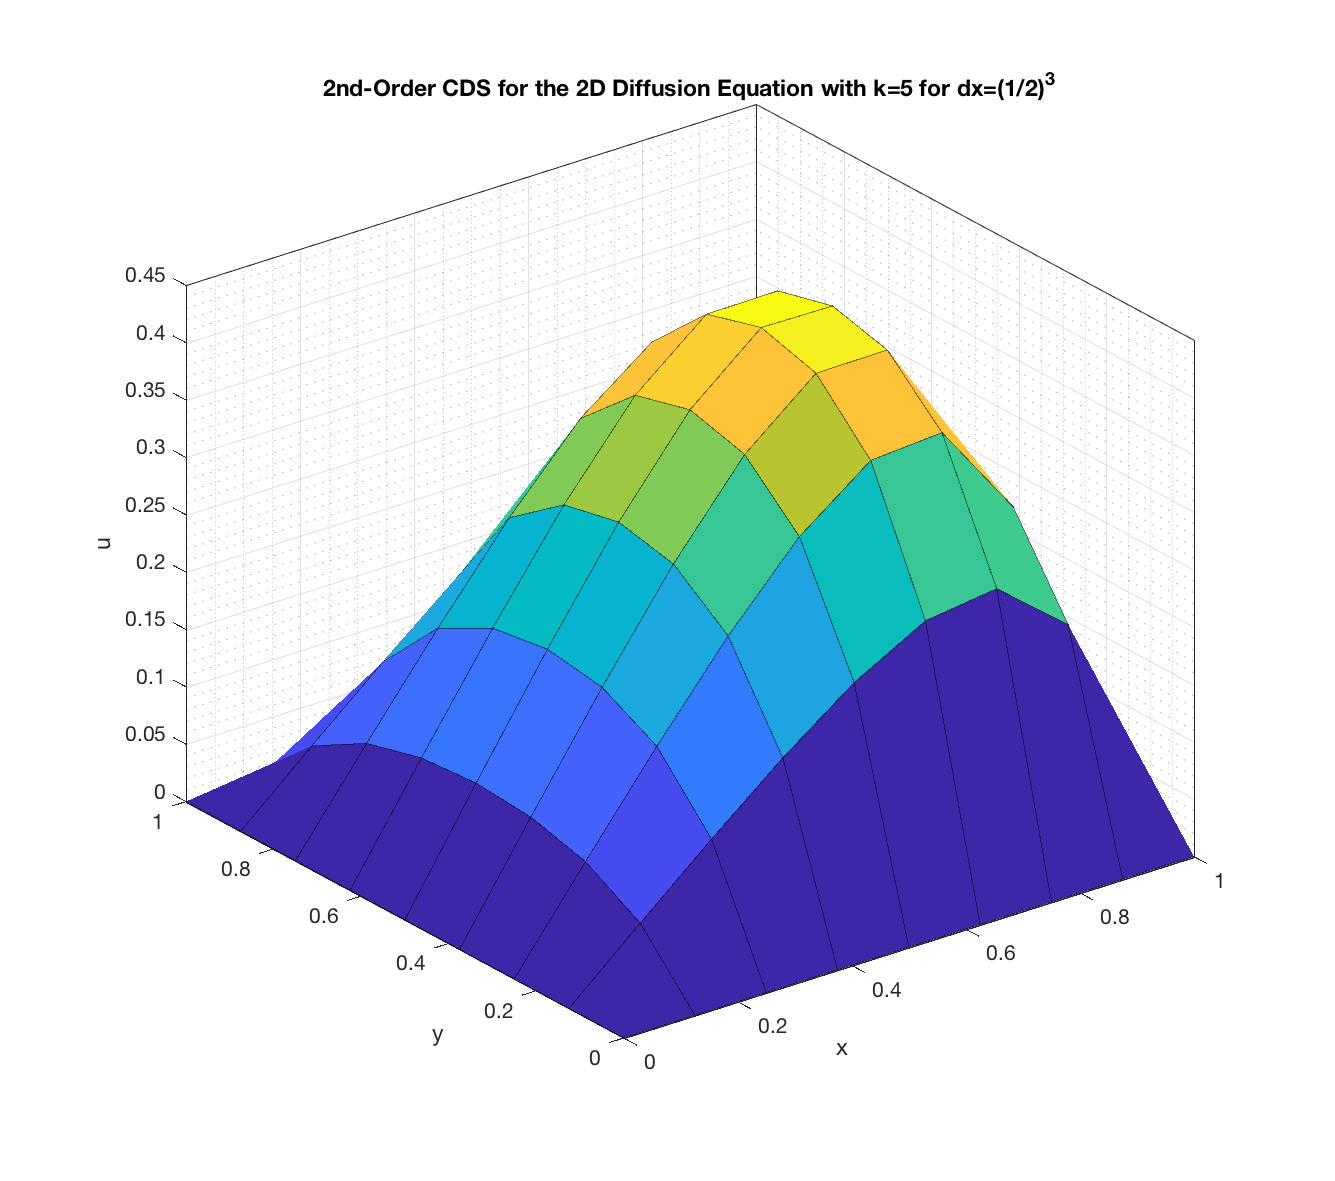
\includegraphics[width = 0.36\linewidth]{surface_minus_order_2_k_5_dx_order_3}
		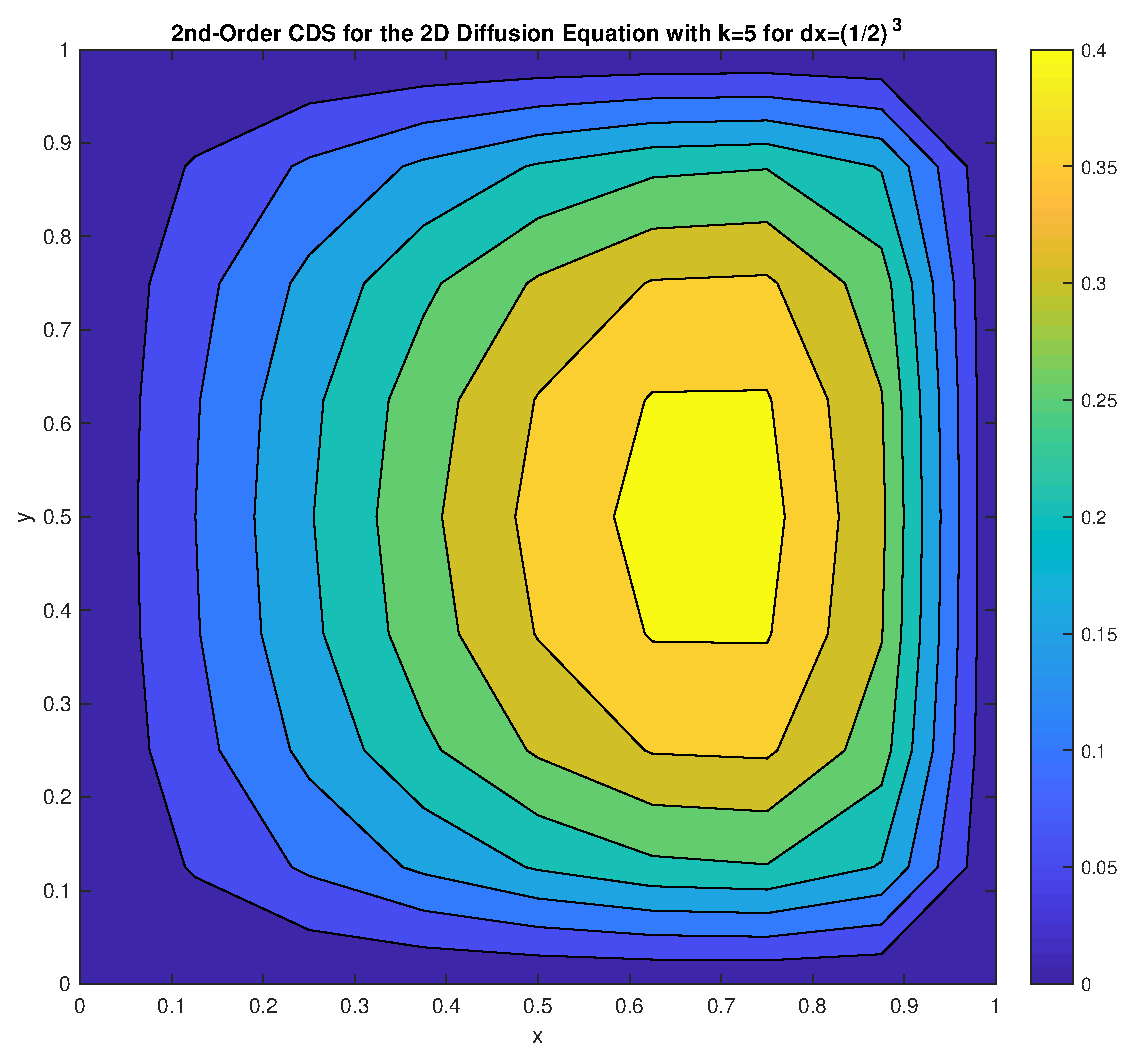
\includegraphics[width = 0.36\linewidth]{contour_minus_order_2_k_5_dx_order_3}
		\caption{2nd-Order CDS for the 2D Diffusion Equation with $k = 5$ for $\Delta x = (1/2)^3$}
	\end{center}
\end{figure}

\begin{figure}[H]
	\begin{center}
		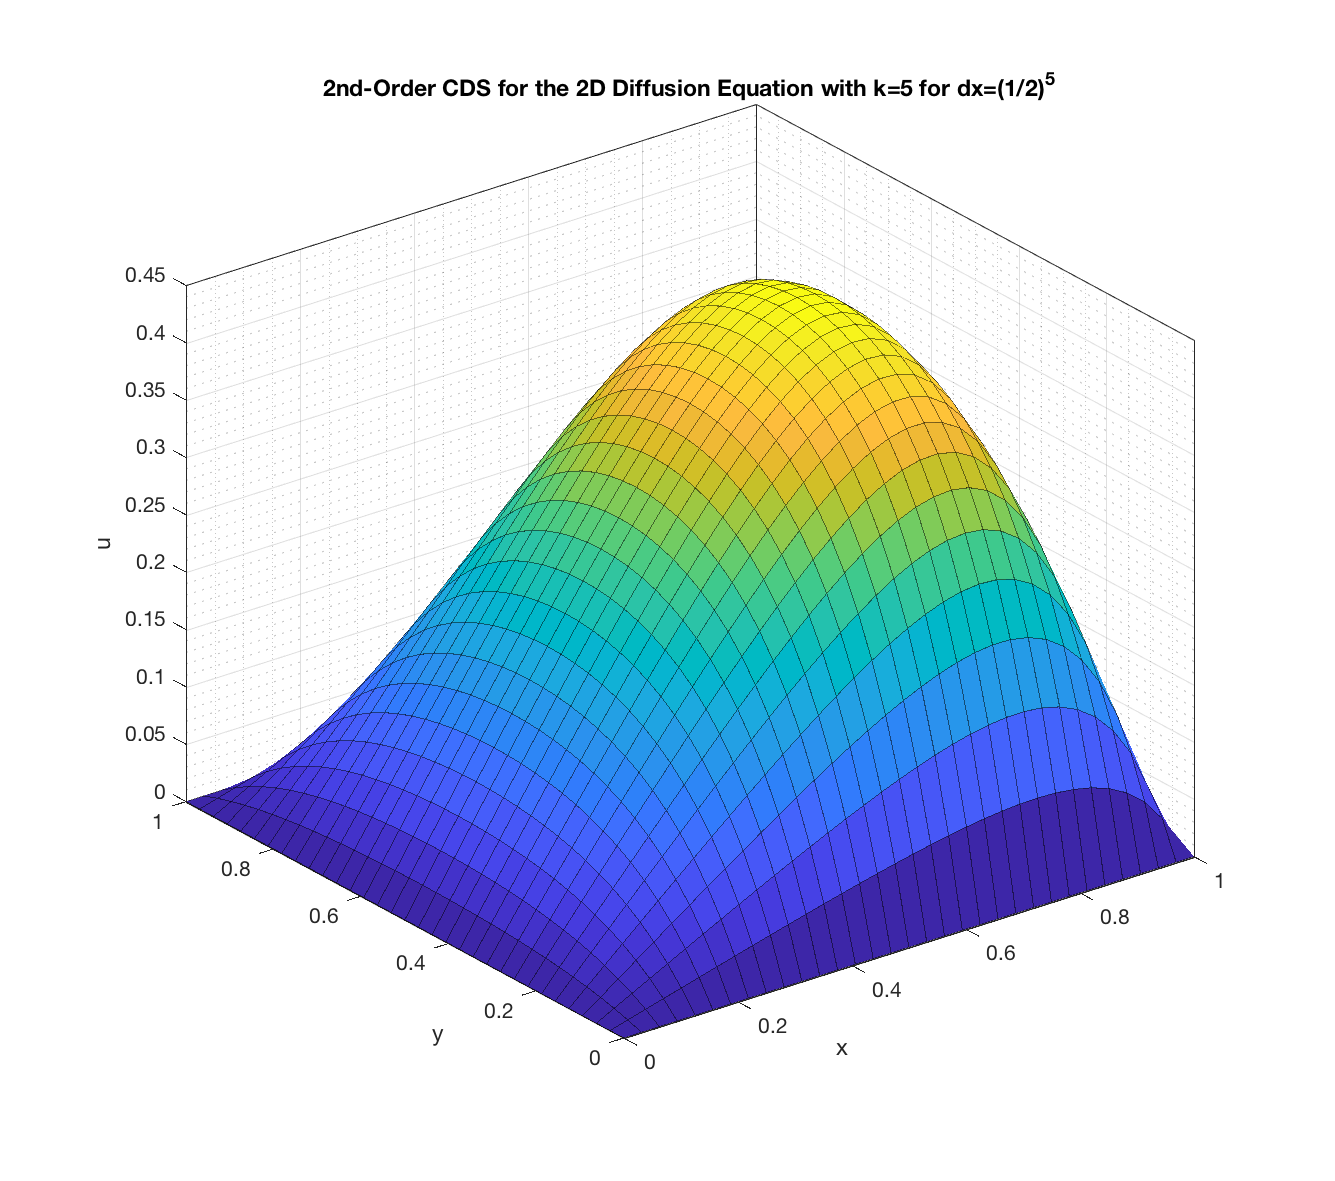
\includegraphics[width = 0.36\linewidth]{surface_minus_order_2_k_5_dx_order_5}
		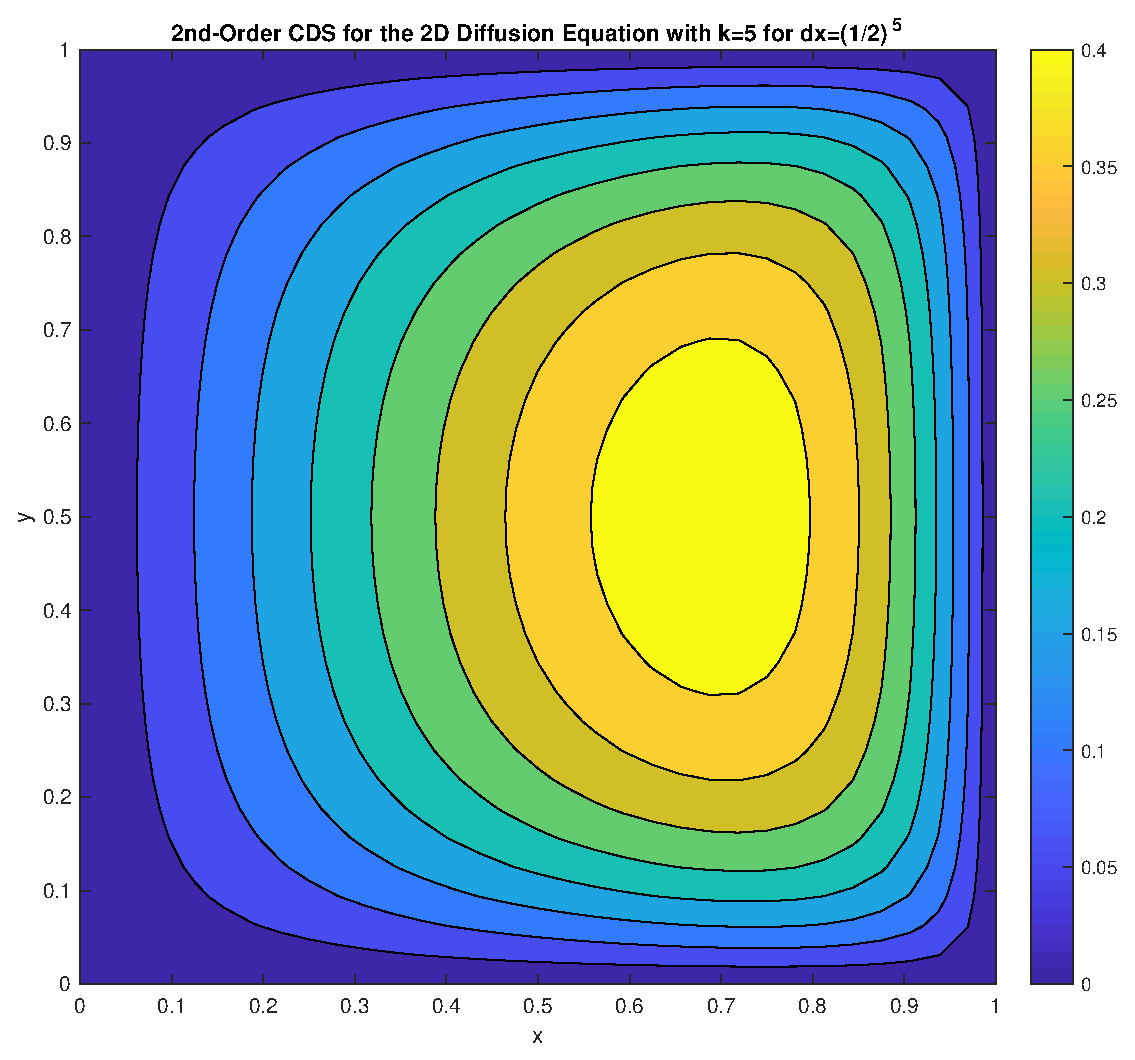
\includegraphics[width = 0.36\linewidth]{contour_minus_order_2_k_5_dx_order_5}
		\caption{2nd-Order CDS for the 2D Diffusion Equation with $k = 5$ for $\Delta x = (1/2)^5$}
	\end{center}
\end{figure}

\begin{figure}[H]
	\begin{center}
		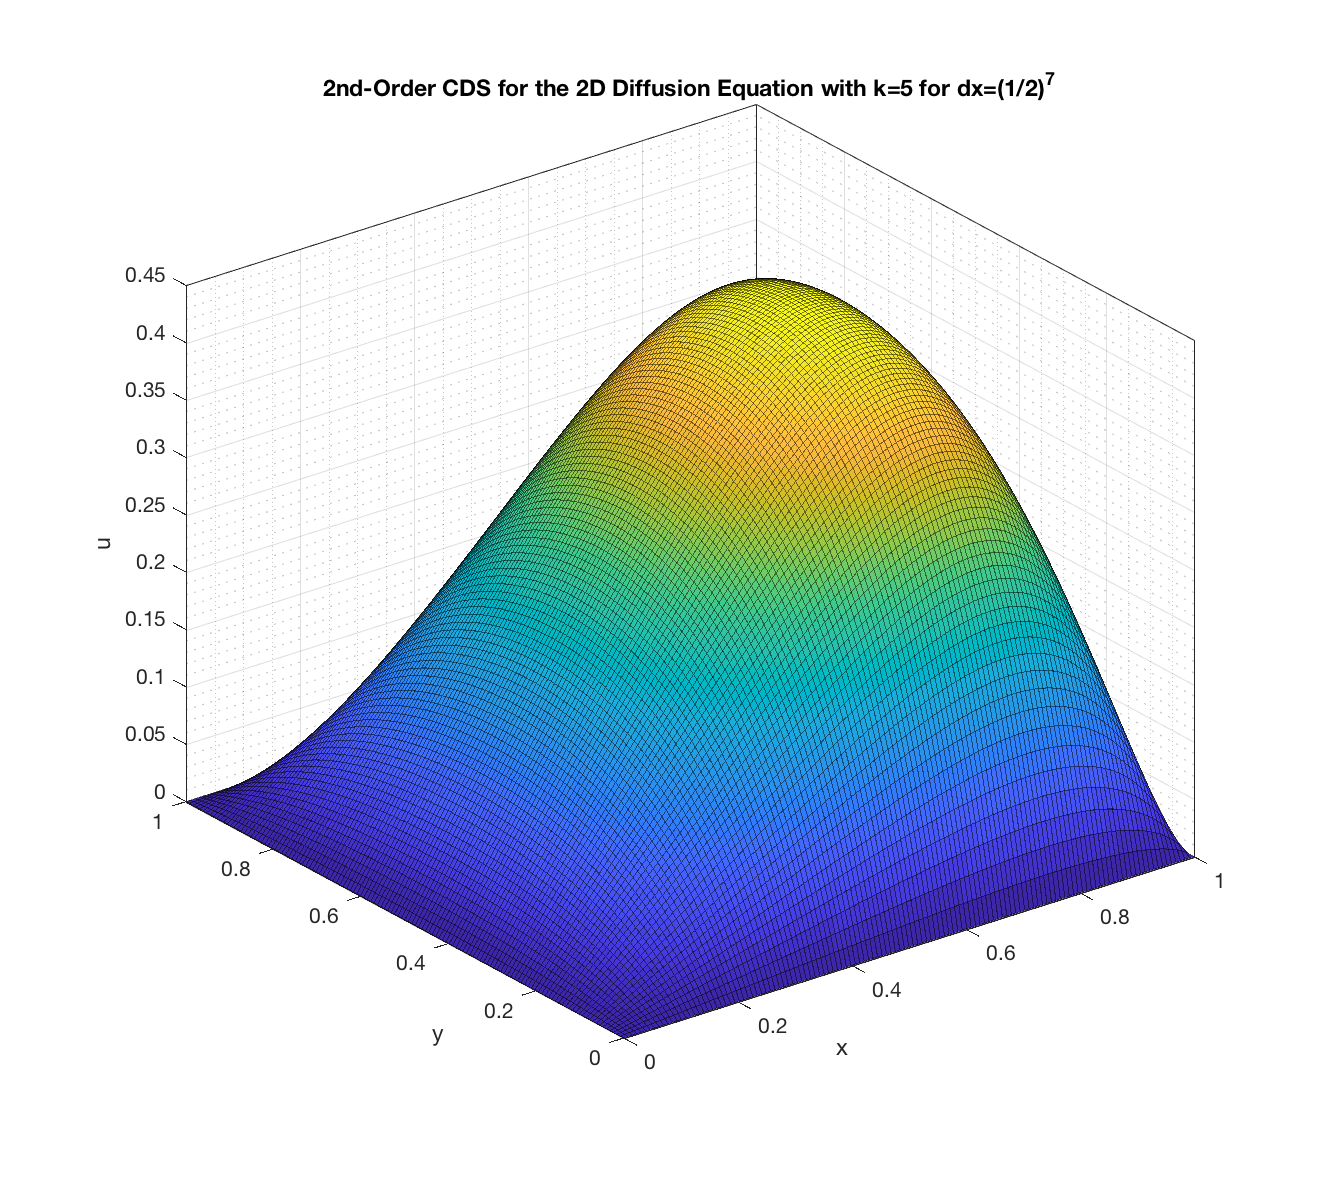
\includegraphics[width = 0.36\linewidth]{surface_minus_order_2_k_5_dx_order_7}
		\includegraphics[width = 0.36\linewidth]{contour_minus_order_2_k_5_dx_order_7}
		\caption{2nd-Order CDS for the 2D Diffusion Equation with $k = 5$ for $\Delta x = (1/2)^7$}
	\end{center}
\end{figure}

\newpage

\begin{figure}[H]
	\begin{center}
		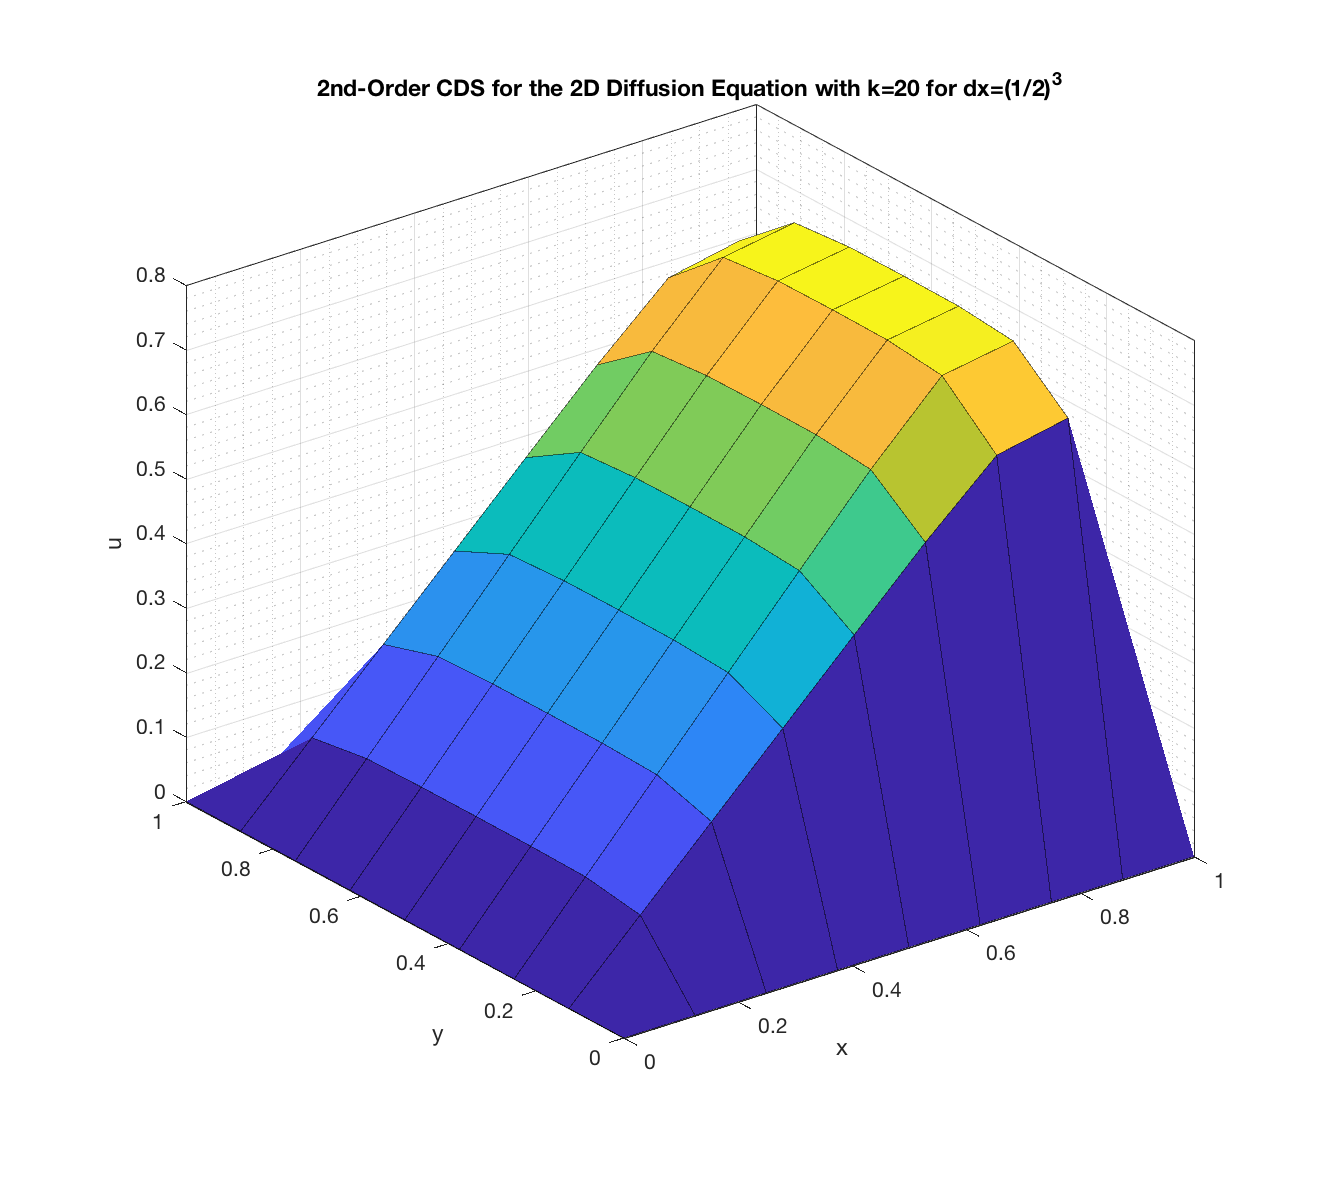
\includegraphics[width = 0.36\linewidth]{surface_minus_order_2_k_20_dx_order_3}
		\includegraphics[width = 0.36\linewidth]{contour_minus_order_2_k_20_dx_order_3}
		\caption{2nd-Order CDS for the 2D Diffusion Equation with $k = 20$ for $\Delta x = (1/2)^3$}
	\end{center}
\end{figure}

\begin{figure}[H]
	\begin{center}
		\includegraphics[width = 0.36\linewidth]{surface_minus_order_2_k_20_dx_order_5}
		\includegraphics[width = 0.36\linewidth]{contour_minus_order_2_k_20_dx_order_5}
		\caption{2nd-Order CDS for the 2D Diffusion Equation with $k = 20$ for $\Delta x = (1/2)^5$}
	\end{center}
\end{figure}

\begin{figure}[H]
	\begin{center}
		\includegraphics[width = 0.36\linewidth]{surface_minus_order_2_k_20_dx_order_7}
		\includegraphics[width = 0.36\linewidth]{contour_minus_order_2_k_20_dx_order_7}
		\caption{2nd-Order CDS for the 2D Diffusion Equation with $k = 20$ for $\Delta x = (1/2)^7$}
	\end{center}
\end{figure}

\newpage

\subsubsection{4th-Order Central Difference Scheme - Diffusion Equation}

\begin{figure}[H]
	\begin{center}
		\includegraphics[width = 0.36\linewidth]{surface_minus_order_4_k_1_dx_order_3}
		\includegraphics[width = 0.36\linewidth]{contour_minus_order_4_k_1_dx_order_3}
		\caption{4th-Order CDS for the 2D Diffusion Equation with $k = 1$ for $\Delta x = (1/2)^3$}
	\end{center}
\end{figure}

\begin{figure}[H]
	\begin{center}
		\includegraphics[width = 0.36\linewidth]{surface_minus_order_4_k_1_dx_order_5}
		\includegraphics[width = 0.36\linewidth]{contour_minus_order_4_k_1_dx_order_5}
		\caption{4th-Order CDS for the 2D Diffusion Equation with $k = 1$ for $\Delta x = (1/2)^5$}
	\end{center}
\end{figure}

\begin{figure}[H]
	\begin{center}
		\includegraphics[width = 0.36\linewidth]{surface_minus_order_4_k_1_dx_order_7}
		\includegraphics[width = 0.36\linewidth]{contour_minus_order_4_k_1_dx_order_7}
		\caption{4th-Order CDS for the 2D Diffusion Equation with $k = 1$ for $\Delta x = (1/2)^7$}
	\end{center}
\end{figure}

\newpage

\begin{figure}[H]
	\begin{center}
		\includegraphics[width = 0.36\linewidth]{surface_minus_order_4_k_5_dx_order_3}
		\includegraphics[width = 0.36\linewidth]{contour_minus_order_4_k_5_dx_order_3}
		\caption{4th-Order CDS for the 2D Diffusion Equation with $k = 5$ for $\Delta x = (1/2)^3$}
	\end{center}
\end{figure}

\begin{figure}[H]
	\begin{center}
		\includegraphics[width = 0.36\linewidth]{surface_minus_order_4_k_5_dx_order_5}
		\includegraphics[width = 0.36\linewidth]{contour_minus_order_4_k_5_dx_order_5}
		\caption{4th-Order CDS for the 2D Diffusion Equation with $k = 5$ for $\Delta x = (1/2)^5$}
	\end{center}
\end{figure}

\begin{figure}[H]
	\begin{center}
		\includegraphics[width = 0.36\linewidth]{surface_minus_order_4_k_5_dx_order_7}
		\includegraphics[width = 0.36\linewidth]{contour_minus_order_4_k_5_dx_order_7}
		\caption{4th-Order CDS for the 2D Diffusion Equation with $k = 5$ for $\Delta x = (1/2)^7$}
	\end{center}
\end{figure}

\newpage

\begin{figure}[H]
	\begin{center}
		\includegraphics[width = 0.36\linewidth]{surface_minus_order_4_k_20_dx_order_3}
		\includegraphics[width = 0.36\linewidth]{contour_minus_order_4_k_20_dx_order_3}
		\caption{4th-Order CDS for the 2D Diffusion Equation with $k = 20$ for $\Delta x = (1/2)^3$}
	\end{center}
\end{figure}

\begin{figure}[H]
	\begin{center}
		\includegraphics[width = 0.36\linewidth]{surface_minus_order_4_k_20_dx_order_5}
		\includegraphics[width = 0.36\linewidth]{contour_minus_order_4_k_20_dx_order_5}
		\caption{4th-Order CDS for the 2D Diffusion Equation with $k = 20$ for $\Delta x = (1/2)^5$}
	\end{center}
\end{figure}

\begin{figure}[H]
	\begin{center}
		\includegraphics[width = 0.36\linewidth]{surface_minus_order_4_k_20_dx_order_7}
		\includegraphics[width = 0.36\linewidth]{contour_minus_order_4_k_20_dx_order_7}
		\caption{4th-Order CDS for the 2D Diffusion Equation with $k = 20$ for $\Delta x = (1/2)^7$}
	\end{center}
\end{figure}

\newpage

\subsection{Finite Difference Method -- Quantity of Interest Results}

\subsubsection{2nd-Order Central Difference Scheme - Wave Equation}

\begin{table}[H]
	\flushleft
	\caption{Quantity of Interest for 2nd-Order CDS FDM for the Wave Equation}		
   \begin{tabular}{|c|c|c|c|c|c|c|}
\hline
\textbf{$\Delta x$}&\textbf{$u'_{k^2=1}(1)$}&\textbf{$u'_{k^2=2}(1)$}&\textbf{$u'_{k^2=5}(1)$}&\textbf{$u'_{k^2=10}(1)$}&\textbf{$u'_{k^2=20}(1)$}&\textbf{$u'_{k^2=50}(1)$}\\\hline
0.5000&0.3167&1.3333&3.4722&23.8095&98.9583&623.9936\\\hline
0.2500&0.2680&1.1759&-3.3701&8.7983&46.8395&309.4743\\\hline
0.1250&0.2585&1.1503&-6.3884&-9.8902&11.4575&149.0340\\\hline
0.0625&0.2566&1.1459&-7.2876&-41.1691&-87.0376&61.0294\\\hline
0.0312&0.2561&1.1450&-7.5237&-87.1428&-103.2300&-193.2596\\\hline
0.0156&0.2560&1.1447&-7.5835&-117.7205&43.6212&119.9487\\\hline
0.0078&0.2560&1.1447&-7.5985&-128.8404&20.7379&1415.2345\\\hline
0.0039&0.2560&1.1447&-7.6023&-131.9439&16.8480&164.3739\\\hline
\end{tabular}

\end{table}

\begin{table}[H]
	\caption{Quantity of Interest for 2nd-Order CDS FDM for the Wave Equation}		
	\begin{tabular}{|c|c|c|c|c|c|c|}
\hline
\textbf{$\Delta x$}&\textbf{$u_{k^2=1}(1/2, 1/2)$}&\textbf{$u_{k^2=2}(1/2, 1/2)$}&\textbf{$u_{k^2=5}(1/2, 1/2)$}&\textbf{$u_{k^2=10}(1/2, 1/2)$}&\textbf{$u_{k^2=20}(1/2, 1/2)$}&\textbf{$u_{k^2=50}(1/2, 1/2)$}\\\hline
0.5000&-0.0333&-0.1667&1.3889&0.5952&0.5208&0.5032\\\hline
0.2500&-0.0373&-0.1818&3.0659&-0.0296&0.4963&0.4999\\\hline
0.1250&-0.0385&-0.1866&3.7317&-3.4967&0.7466&0.5000\\\hline
0.0625&-0.0389&-0.1878&3.9300&-12.7551&3.5629&0.5000\\\hline
0.0312&-0.0389&-0.1882&3.9820&-26.7039&1.3393&6.2240\\\hline
0.0156&-0.0390&-0.1882&3.9952&-36.0198&1.1892&-0.8313\\\hline
0.0078&-0.0390&-0.1883&3.9985&-39.4104&1.1571&-0.6232\\\hline
0.0039&-0.0390&-0.1883&3.9993&-40.3569&1.1494&-0.7898\\\hline
\end{tabular}

\end{table}

\subsubsection{4th-Order Central Difference Scheme - Wave Equation}

\begin{table}[H]
	\caption{Quantity of Interest for 4th-Order CDS FDM for the Wave Equation}		
	\begin{tabular}{|c|c|c|c|c|c|c|}
\hline
\textbf{$\Delta x$}&\textbf{$u_{k^2=1}(1/2, 1/2)$}&\textbf{$u_{k^2=2}(1/2, 1/2)$}&\textbf{$u_{k^2=5}(1/2, 1/2)$}&\textbf{$u_{k^2=10}(1/2, 1/2)$}&\textbf{$u_{k^2=20}(1/2, 1/2)$}&\textbf{$u_{k^2=50}(1/2, 1/2)$}\\\hline
0.5000&-0.0395&-0.1875&3.7500&0.9375&0.7895&0.7560\\\hline
0.2500&-0.0390&-0.1882&3.9923&-2.1800&0.4596&0.4788\\\hline
0.1250&-0.0390&-0.1883&3.9992&-27.1000&-1.2494&0.4993\\\hline
0.0625&-0.0390&-0.1883&3.9995&-39.5289&1.1932&0.9439\\\hline
0.0312&-0.0390&-0.1883&3.9996&-40.6093&1.1494&-0.1117\\\hline
0.0156&-0.0390&-0.1883&3.9996&-40.6777&1.1470&-0.8153\\\hline
0.0078&-0.0390&-0.1883&3.9996&-40.6820&1.1468&-0.9162\\\hline
0.0039&-0.0390&-0.1883&3.9996&-40.6823&1.1468&-0.9228\\\hline
\end{tabular}

\end{table}

\newpage

\subsubsection{2nd-Order Central Difference Scheme - Diffusion Equation}

\begin{table}[H]
	\flushleft
	\caption{Quantity of Interest for 2nd-Order CDS FDM for the Diffusion Equation}		
	\begin{tabular}{|c|c|c|c|c|c|c|}
\hline
\textbf{$\Delta x$}&\textbf{$u'_{k^2=1}(1)$}&\textbf{$u'_{k^2=2}(1)$}&\textbf{$u'_{k^2=5}(1)$}&\textbf{$u'_{k^2=10}(1)$}&\textbf{$u'_{k^2=20}(1)$}&\textbf{$u'_{k^2=50}(1)$}\\\hline
0.5000&-0.3088&-1.2000&-6.8598&-25.8621&-100.9615&-625.9936\\\hline
0.2500&-0.2549&-0.9575&-4.6996&-14.9492&-52.8445&-315.4745\\\hline
0.1250&-0.2435&-0.9013&-4.0475&-10.7511&-31.0138&-163.0551\\\hline
0.0625&-0.2410&-0.8886&-3.8762&-9.4439&-22.5843&-91.7551\\\hline
0.0312&-0.2404&-0.8855&-3.8327&-9.0906&-19.9534&-62.4498\\\hline
0.0156&-0.2403&-0.8847&-3.8218&-9.0003&-19.2423&-52.6793\\\hline
0.0078&-0.2402&-0.8845&-3.8191&-8.9776&-19.0606&-49.9447\\\hline
0.0039&-0.2402&-0.8845&-3.8184&-8.9720&-19.0149&-49.2379\\\hline
\end{tabular}

\end{table}

\begin{table}[H]
	\caption{Quantity of Interest for 4th-Order CDS FDM for the Wave Equation}		
	\begin{tabular}{|c|c|c|c|c|c|c|}
\hline
\textbf{$\Delta x$}&\textbf{$u_{k^2=1}(1/2, 1/2)$}&\textbf{$u_{k^2=2}(1/2, 1/2)$}&\textbf{$u_{k^2=5}(1/2, 1/2)$}&\textbf{$u_{k^2=10}(1/2, 1/2)$}&\textbf{$u_{k^2=20}(1/2, 1/2)$}&\textbf{$u_{k^2=50}(1/2, 1/2)$}\\\hline
0.5000&0.0294&0.1000&0.3049&0.4310&0.4808&0.4968\\\hline
0.2500&0.0332&0.1142&0.3501&0.4714&0.4973&0.4999\\\hline
0.1250&0.0345&0.1188&0.3656&0.4832&0.4995&0.5000\\\hline
0.0625&0.0348&0.1200&0.3699&0.4863&0.4998&0.5000\\\hline
0.0312&0.0349&0.1203&0.3710&0.4871&0.4999&0.5000\\\hline
0.0156&0.0349&0.1204&0.3713&0.4873&0.4999&0.5000\\\hline
0.0078&0.0349&0.1204&0.3714&0.4873&0.4999&0.5000\\\hline
0.0039&0.0349&0.1204&0.3714&0.4873&0.4999&0.5000\\\hline
\end{tabular}

\end{table}

\subsubsection{4th-Order Central Difference Scheme - Diffusion Equation}

\begin{table}[H]
	\caption{Quantity of Interest for 4th-Order CDS FDM for the Wave Equation}		
	\begin{tabular}{|c|c|c|c|c|c|c|}
\hline
\textbf{$\Delta x$}&\textbf{$u_{k^2=1}(1/2, 1/2)$}&\textbf{$u_{k^2=2}(1/2, 1/2)$}&\textbf{$u_{k^2=5}(1/2, 1/2)$}&\textbf{$u_{k^2=10}(1/2, 1/2)$}&\textbf{$u_{k^2=20}(1/2, 1/2)$}&\textbf{$u_{k^2=50}(1/2, 1/2)$}\\\hline
0.5000&0.0357&0.1250&0.4167&0.6250&0.7143&0.7440\\\hline
0.2500&0.0350&0.1207&0.3740&0.4924&0.4962&0.4852\\\hline
0.1250&0.0349&0.1204&0.3715&0.4877&0.5000&0.5000\\\hline
0.0625&0.0349&0.1204&0.3714&0.4874&0.4999&0.5000\\\hline
0.0312&0.0349&0.1204&0.3714&0.4874&0.4999&0.5000\\\hline
0.0156&0.0349&0.1204&0.3714&0.4874&0.4999&0.5000\\\hline
0.0078&0.0349&0.1204&0.3714&0.4874&0.4999&0.5000\\\hline
0.0039&0.0349&0.1204&0.3714&0.4874&0.4999&0.5000\\\hline
\end{tabular}

\end{table}

\newpage

\section{Convergence Analysis}

\subsection{Rate of Convergence Derivation}

Let the error for a particular mesh size $\Delta x$ be $E\left(\Delta x\right)$:
\begin{equation}
E\left(\Delta x\right) = C\left(\Delta x\right)^\beta
\end{equation}
Then for a smaller mesh size $\frac{\Delta x}{2}$ we have:
\begin{equation}
E\left(\frac{\Delta x}{2}\right) = C\left(\frac{\Delta x}{2}\right)^\beta
\end{equation}
Dividing the error at each mesh size and taking the logarithm:
\begin{equation}
\frac{E\left(\Delta x\right)}{E\left(\frac{\Delta x}{2}\right)} = \frac{C\left(\Delta x\right)^\beta}{C\left(\frac{\Delta x}{2}\right)^\beta} = 2^\beta
\end{equation}
\begin{equation}
\log\left[\frac{E\left(\Delta x\right)}{E\left(\frac{\Delta x}{2}\right)}\right] = \log(2^\beta)
\end{equation}
\begin{equation}
\log\left[\frac{E\left(\Delta x\right)}{E\left(\frac{\Delta x}{2}\right)}\right] = \beta \log(2)
\end{equation}
Rearranging for $\beta$ and simplifying:
\begin{equation}
\beta = \frac{1}{\log(2)} \left[\log\left(E\left(\Delta x\right)\right) - \log\left(E\left(\frac{\Delta x}{2}\right)\right)\right] 
\end{equation}
Denoting $E^*_{\Delta x} = \log\left(E\left(\Delta x\right)\right)$:
\begin{equation}
\mathbf{\beta = \frac{E^*_{\Delta x} - E^*_{\frac{\Delta x}{2}}}{\log (2)}}
\end{equation}

\newpage

\subsection{Rate of Convergence for the Wave Equation -- Results}

\subsubsection{2nd-Order Central Difference Scheme}

\begin{figure}[H]
	\begin{center}
		\includegraphics[width = 0.8\linewidth]{plus_order_2_u_avg}
		\caption{Rate of Convergence of $u(1/2, 1/2)$ for 2nd-Order CDS FDM for the Wave Equation for Several Values of $k^2$}	
	\end{center}
\end{figure}

\begin{table}[H]
	\begin{tabular}{|c|c|c|c|c|c|c|}
\hline
\textbf{$\Delta x$}&\textbf{$\beta(k^2=1)$}&\textbf{$\beta(k^2=2)$}&\textbf{$\beta(k^2=5)$}&\textbf{$\beta(k^2=10)$}&\textbf{$\beta(k^2=20)$}&\textbf{$\beta(k^2=50)$}\\\hline
0.5000&1.7388&1.7372&1.4834&0.0220&-0.0555&0.0033\\\hline
0.2500&1.9203&1.9226&1.8012&0.1286&0.7009&-0.0001\\\hline
0.1250&1.9787&1.9795&1.9452&0.4131&-2.5938&-0.0000\\\hline
0.0625&1.9946&1.9948&1.9859&0.9985&3.6502&-2.3282\\\hline
0.0312&1.9986&1.9987&1.9965&1.5840&2.1846&6.2799\\\hline
0.0156&1.9997&1.9997&1.9991&1.8741&2.0386&-1.7061\\\hline
0.0078&2.0001&2.0001&1.9998&1.9667&2.0092&1.1693\\\hline
\end{tabular}

\end{table}

\newpage

\subsubsection{4th-Order Central Difference Scheme}

\begin{figure}[H]
	\begin{center}
		\includegraphics[width = 0.8\linewidth]{plus_order_4_u_avg}
		\caption{Rate of Convergence of $u(1/2, 1/2)$ for 4th-Order CDS FDM for the Wave Equation for Several Values of $k^2$}	
	\end{center}
\end{figure}

\begin{table}[H]
	\begin{tabular}{|c|c|c|c|c|c|c|}
\hline
\textbf{$\Delta x$}&\textbf{$\beta(k^2=1)$}&\textbf{$\beta(k^2=2)$}&\textbf{$\beta(k^2=5)$}&\textbf{$\beta(k^2=10)$}&\textbf{$\beta(k^2=20)$}&\textbf{$\beta(k^2=50)$}\\\hline
0.5000&4.1885&3.4160&5.0988&0.1123&-0.9434&0.2603\\\hline
0.2500&4.1145&3.8041&4.3841&1.5032&-1.8019&-0.0209\\\hline
0.1250&4.0305&3.9550&4.1070&3.5578&5.6901&-0.3924\\\hline
0.0625&4.0061&3.9909&4.0273&3.9816&4.1718&1.2021\\\hline
0.0312&3.9731&4.0311&4.0034&4.0024&4.0235&2.9107\\\hline
0.0156&3.6026&4.6881&3.9461&4.0010&4.0052&3.9294\\\hline
0.0078&1.7198&0.8616&3.3055&4.0003&4.0082&3.9998\\\hline
\end{tabular}

\end{table}

\newpage

\subsection{Rate of Convergence for the Diffusion Equation -- Results}

\subsubsection{2nd-Order Central Difference Scheme}

\begin{figure}[H]
	\begin{center}
				\includegraphics[width = 0.8\linewidth]{minus_order_2_u_avg}
		\caption{Rate of Convergence of $u(1/2, 1/2)$ for 2nd-Order CDS FDM for the Diffusion Equation for Several Values of $k^2$}	
	\end{center}
\end{figure}

\begin{table}[H]
		\begin{tabular}{|c|c|c|c|c|c|c|}
\hline
\textbf{$\Delta x$}&\textbf{$\beta(k^2=1)$}&\textbf{$\beta(k^2=2)$}&\textbf{$\beta(k^2=5)$}&\textbf{$\beta(k^2=10)$}&\textbf{$\beta(k^2=20)$}&\textbf{$\beta(k^2=50)$}\\\hline
0.5000&1.7279&1.7095&1.6461&1.8156&2.8570&5.3183\\\hline
0.2500&1.9158&1.9082&1.8736&1.9420&2.8514&7.1949\\\hline
0.1250&1.9774&1.9751&1.9637&1.9827&2.4390&1.8070\\\hline
0.0625&1.9942&1.9936&1.9905&1.9953&2.1467&-0.0507\\\hline
0.0312&1.9986&1.9984&1.9976&1.9989&2.0469&-0.0014\\\hline
0.0156&1.9997&1.9996&1.9995&2.0001&2.0409&-0.0002\\\hline
0.0078&2.0001&2.0001&2.0001&2.0016&2.1331&-0.0000\\\hline
\end{tabular}

\end{table}

\newpage

\subsubsection{4th-Order Central Difference Scheme}

\begin{figure}[H]
	\begin{center}
				\includegraphics[width = 0.8\linewidth]{minus_order_4_u_avg}
		\caption{Rate of Convergence of $u(1/2, 1/2)$ for 4th-Order CDS FDM for the Diffusion Equation for Several Values of $k^2$}	
	\end{center}
\end{figure}

\begin{table}[H]
		\begin{tabular}{|c|c|c|c|c|c|c|}
\hline
\textbf{$\Delta x$}&\textbf{$\beta(k^2=1)$}&\textbf{$\beta(k^2=2)$}&\textbf{$\beta(k^2=5)$}&\textbf{$\beta(k^2=10)$}&\textbf{$\beta(k^2=20)$}&\textbf{$\beta(k^2=50)$}\\\hline
0.5000&4.0886&4.0505&4.1000&4.7734&5.8662&4.0432\\\hline
0.2500&4.0531&4.0252&3.9778&3.8825&6.1578&8.7139\\\hline
0.1250&4.0131&4.0054&3.9883&3.9445&3.5637&7.7727\\\hline
0.0625&3.9957&3.9962&3.9935&3.9783&3.8082&0.0002\\\hline
0.0312&3.8806&3.9184&3.9475&3.9003&2.8262&0.0001\\\hline
0.0156&2.8113&3.0869&3.3558&2.9801&0.7027&0.0000\\\hline
0.0078&0.6804&0.9116&1.2427&0.8134&0.0579&0.0000\\\hline
\end{tabular}

\end{table}

\newpage

\section{Discussion}

In solution of the 2D wave equation and the 2D diffusion equation, meshes were computed down to a grid spacing of $\Delta x = (1/2)^8$. At this limit the computation time begins to bear the limit of the computer. In the future, a banded or multi-frontal solver could be employed for further benefit and to extend the results to smaller grid spacings. There is, however, no reduction in quality of the results for the solution of the interior finite difference equations using the current method.

Construction of the exact solution was completed using an expansion of the Fourier double sine series, which naturally satisfies the boundary conditions $u\big|_{\partial \Omega}$. Application of Galerkin orthogonality condition allows the Fourier coefficients to be calculated based on the arithmetic of the partial differential equation. This double series approaches the exact solution when the number of terms approaches infinity. Since estimation of the exact solution with high precision is necessary in calculating rates of convergence, determining the appropriate truncation of the double series is critical in achieving the proper precision to develop accurate results. Upon further inspection, it is seen that for any even integer, the double series must be zero. This reduces the computation time fourfold and allows higher precision to be obtained. In our case, the truncation limit was 10,000 terms, yielding an approximation comprised of 5,000 x 5,000 = 25 million terms. It is assumed and verified that this is sufficient to achieve the desired results.

For the 2nd-order central difference schemes for both the 2D wave equation and the 2D diffusion equation, second-order convergence of the grid is observed. This is notable since the method for construction of the exact solution was a Fourier double sine series. Local point convergence was seen as well as estimated convergence of the partial derivative at the right boundary with similar second-order convergence characteristics.

For the 4th-order central difference schemes for both the 2D wave equation and the 2D diffusion equation, fourth-order convergence of the grid is observed. This is notable since the method for construction of the exact solution was a Fourier double sine series. Local point convergence was seen as well as estimated convergence of the partial derivative at the right boundary with similar fourth-order convergence characteristics.

In general, the behavior of $k$ values near to unity yields traditional, smooth convergence curves, while high $k$ values are not particularly well-behaves (as $k=50$). For larger $k$ values, we observe a locking phenomenon that requires necessary grid spacing for the error to begin decreasing. This is visualized as a plateau at low grid spacings for high $k$ values. For the diffusion equation, we observe a nominal convergence behavior for all cases except $k = 50$ which apparently converges more quickly and is captured by roundoff earlier. It is assumed that this is spurious and due to eigenvalue resonance causing the solution to be approximated with littie initial error.

A comparison of all of the methods for various values of $k$ proves that:

\begin{itemize}
	\item the second-order central difference scheme finite difference method is quadratically convergent
	\item the fourth-order central difference scheme finite difference method is quartically convergent
\end{itemize}

\newpage

\appendix

\section{MATLAB Code}

\subsection{homework\_6\_plus\_order\_2.m}

\begin{lstlisting}
clear all; close all; clc
%#ok<*SPRIX>
%#ok<*CTCH>
%#ok<*UNRCH>
%#ok<*CLALL>
%#ok<*SAGROW>

%% 2nd-Order

meshOrder   = 1:8;
meshDx      = 1./(2.^meshOrder);

kVals       = [1 2 5 10 20 50];

genFigSurface   = 0;
genFigContour   = 0;
genFigAvg       = 0;
tableSave       = 0;

rowID = 0;
colID = 0;

matNumTotal = numel(meshOrder)*numel(kVals);
matNum = 0;

for k = kVals

rowID = rowID + 1;
colID = 0;

for order = meshOrder

matNum = matNum + 1;

clc
fprintf('solving matrix %i/%i\n', matNum, matNumTotal)

colID = colID + 1;

clear A ARow b u U

dx = 1/(2^order);
n = 1/dx;

A = assemblePlus(dx, n, k, 2);

xi = k^2*dx^2*linspace(0+dx, 1-dx, n-1)';

for i = 1:(n-1)
if i == 1
b = xi;
else
b = [b; xi];
end
end

u = A\b;

u = reshape(u, n-1, n-1)';
U = zeros(n+1, n+1);
U(2:end-1, 2:end-1) = u;

x = linspace(0, 1, n+1);
y = linspace(0, 1, n+1);

[X, Y] = meshgrid(x, y);

titleString = strcat('2nd-Order CDS for the 2D Wave Equation with k=', ...
num2str(k), ' for dx=(1/2)^', num2str(order));
figureString = strcat('plus_order_2_k_', num2str(k), '_dx_order_', num2str(order));

if genFigSurface
figSurface(X, Y, U, titleString, figureString);
end

if genFigContour
figContour(X, Y, U, titleString, figureString);
end

[dim, ~] = size(U);
avg = (dim+1)/2;

uavgfdm(rowID, colID) = U(avg, avg);
[uavgexact(rowID, colID), ~] = exactSolution(k, 1/2, 1/2, 1000);
uxfdm(rowID, colID) = 1 / dx * - U(avg, end-1) + k^2*dx/2*1;
[uxexact(rowID, colID), ~] = exactDerivative(k, 1, 1/2, 1000);

end

end

relErrorAvg = abs(uavgexact-uavgfdm) ./ abs(uavgexact) * 100;
logRelErrorAvg = log10(relErrorAvg);

for kID = 1:numel(kVals)
for rocID = 1:length(logRelErrorAvg) - 1
rocAvg(kID, rocID) = (logRelErrorAvg(kID, rocID+1) - logRelErrorAvg(kID, rocID)) / -log10(2);
end
end

if genFigAvg
figAvg(2, meshDx, relErrorAvg);
end

if tableSave
tableRender(2, meshDx, 0, rocAvg, uxfdm, 0, 0, uavgfdm);
end
\end{lstlisting}

\subsection{homework\_6\_plus\_order\_4.m}

\begin{lstlisting}
clear all; close all; clc
%#ok<*SPRIX>
%#ok<*CTCH>
%#ok<*UNRCH>
%#ok<*CLALL>
%#ok<*SAGROW>

%% 4th-Order

meshOrder   = 1:8;
meshDx      = 1./(2.^meshOrder);

kVals       = [1 2 5 10 20 50];

genFigSurface   = 0;
genFigContour   = 0;
genFigAvg       = 0;
tableSave       = 0;

rowID = 0;
colID = 0;

matNumTotal = numel(meshOrder)*numel(kVals);
matNum = 0;

for k = kVals

rowID = rowID + 1;
colID = 0;

for order = meshOrder

matNum = matNum + 1;

clc
fprintf('solving matrix %i/%i\n', matNum, matNumTotal)

colID = colID + 1;

clear A ARow b u U C d ux

dx = 1/(2^order);
n = 1/dx;

A = assemblePlus(dx, n, k, 4);

xi = k^2*dx^2*linspace(0+dx, 1-dx, n-1)';

for i = 1:(n-1)
if i == 1
b = xi;
else
b = [b; xi];
end
end

u = A\b;

u = reshape(u, n-1, n-1)';
U = zeros(n+1, n+1);
U(2:end-1, 2:end-1) = u;

x = linspace(0, 1, n+1);
y = linspace(0, 1, n+1);

[X, Y] = meshgrid(x, y);

titleString = strcat('4th-Order CDS for the 2D Wave Equation with k=', ...
num2str(k), ' for dx=(1/2)^', num2str(order));
figureString = strcat('plus_order_4_k_', num2str(k), '_dx_order_', num2str(order));

if genFigSurface
figSurface(X, Y, U, titleString, figureString);
end

if genFigContour
figContour(X, Y, U, titleString, figureString);
end

[dim, ~] = size(U);
avg = (dim+1)/2;

uavgfdm(rowID, colID) = U(avg, avg);
[uavgexact(rowID, colID), ~] = exactSolution(k, 1/2, 1/2, 1000);

end

end

relErrorAvg = abs(uavgexact-uavgfdm) ./ abs(uavgexact) * 100;
logRelErrorAvg = log10(relErrorAvg);

for kID = 1:numel(kVals)
for rocID = 1:length(logRelErrorAvg) - 1
rocAvg(kID, rocID) = (logRelErrorAvg(kID, rocID+1) - logRelErrorAvg(kID, rocID)) / -log10(2);
end
end

if genFigAvg
figAvg(4, meshDx, relErrorAvg);
end

if tableSave
tableRender(4, meshDx, 0, rocAvg, 0, 0, 0, uavgfdm);
end
\end{lstlisting}

\subsection{homework\_6\_minus\_order\_2.m}

\begin{lstlisting}
clear all; close all; clc
%#ok<*SPRIX>
%#ok<*CTCH>
%#ok<*UNRCH>
%#ok<*CLALL>
%#ok<*SAGROW>

%% 2nd-Order

meshOrder   = 1:8;
meshDx      = 1./(2.^meshOrder);

kVals       = [1 2 5 10 20 50];

genFigSurface   = 0;
genFigContour   = 0;
genFigAvg       = 0;
tableSave       = 0;

rowID = 0;
colID = 0;

matNumTotal = numel(meshOrder)*numel(kVals);
matNum = 0;

for k = kVals

rowID = rowID + 1;
colID = 0;

for order = meshOrder

matNum = matNum + 1;

clc
fprintf('solving matrix %i/%i\n', matNum, matNumTotal)

colID = colID + 1;

clear A ARow b u U

dx = 1/(2^order);
n = 1/dx;

A = assembleMinus(dx, n, k, 2);

xi = k^2*dx^2*linspace(0+dx, 1-dx, n-1)';

for i = 1:(n-1)
if i == 1
b = xi;
else
b = [b; xi];
end
end

u = A\b;

u = reshape(u, n-1, n-1)';
U = zeros(n+1, n+1);
U(2:end-1, 2:end-1) = u;

x = linspace(0, 1, n+1);
y = linspace(0, 1, n+1);

[X, Y] = meshgrid(x, y);

titleString = strcat('2nd-Order CDS for the 2D Diffusion Equation with k=', ...
num2str(k), ' for dx=(1/2)^', num2str(order));
figureString =  strcat('minus_order_2_k_', num2str(k), '_dx_order_', num2str(order));

if genFigSurface
figSurface(X, Y, U, titleString, figureString);
end

if genFigContour
figContour(X, Y, U, titleString, figureString);
end

[dim, ~] = size(U);
avg = (dim+1)/2;

uavgfdm(rowID, colID) = U(avg, avg);
[~, uavgexact(rowID, colID)] = exactSolution(k, 1/2, 1/2, 1000);
uxfdm(rowID, colID) = 1 / dx * - U(avg, end-1) - k^2*dx/2*1;
[~, uxexact(rowID, colID)] = exactDerivative(k, 1, 1/2, 1000);

end

end

relErrorAvg = abs(uavgexact-uavgfdm) ./ abs(uavgexact) * 100;
logRelErrorAvg = log10(relErrorAvg);

for kID = 1:numel(kVals)
for rocID = 1:length(logRelErrorAvg) - 1
rocAvg(kID, rocID) = (logRelErrorAvg(kID, rocID+1) - logRelErrorAvg(kID, rocID)) / -log10(2);
end
end

if genFigAvg
figAvg(2, meshDx, relErrorAvg);
end

if tableSave
tableRender(2, meshDx, 0, rocAvg, uxfdm, 0, 0, uavgfdm);
end
\end{lstlisting}

\subsection{homework\_6\_minus\_order\_4.m}

\begin{lstlisting}
clear all; close all; clc
%#ok<*SPRIX>
%#ok<*CTCH>
%#ok<*UNRCH>
%#ok<*CLALL>
%#ok<*SAGROW>

%% 4th-Order

meshOrder   = 1:8;
meshDx      = 1./(2.^meshOrder);

kVals       = [1 2 5 10 20 50];

genFigSurface   = 0;
genFigContour   = 0;
genFigAvg       = 0;
tableSave       = 0;

rowID = 0;
colID = 0;

matNumTotal = numel(meshOrder)*numel(kVals);
matNum = 0;

for k = kVals

rowID = rowID + 1;
colID = 0;

for order = meshOrder

matNum = matNum + 1;

clc
fprintf('solving matrix %i/%i\n', matNum, matNumTotal)

colID = colID + 1;

clear A ARow b u U C d ux

dx = 1/(2^order);
n = 1/dx;

A = assembleMinus(dx, n, k, 4);

xi = k^2*dx^2*linspace(0+dx, 1-dx, n-1)';

for i = 1:(n-1)
if i == 1
b = xi;
else
b = [b; xi];
end
end

u = A\b;

u = reshape(u, n-1, n-1)';
U = zeros(n+1, n+1);
U(2:end-1, 2:end-1) = u;

x = linspace(0, 1, n+1);
y = linspace(0, 1, n+1);

[X, Y] = meshgrid(x, y);

titleString = strcat('4th-Order CDS for the 2D Diffusion Equation with k=', ...
num2str(k), ' for dx=(1/2)^', num2str(order));
figureString = strcat('minus_order_4_k_', num2str(k), '_dx_order_', num2str(order));

if genFigSurface
figSurface(X, Y, U, titleString, figureString);
end

if genFigContour
figContour(X, Y, U, titleString, figureString);
end

[dim, ~] = size(U);
avg = (dim+1)/2;

uavgfdm(rowID, colID) = U(avg, avg);
[~, uavgexact(rowID, colID)] = exactSolution(k, 1/2, 1/2, 1000);

end

end

relErrorAvg = abs(uavgexact-uavgfdm) ./ abs(uavgexact) * 100;
logRelErrorAvg = log10(relErrorAvg);

for kID = 1:numel(kVals)
for rocID = 1:length(logRelErrorAvg) - 1
rocAvg(kID, rocID) = (logRelErrorAvg(kID, rocID+1) - logRelErrorAvg(kID, rocID)) / -log10(2);
end
end

if genFigAvg
figAvg(4, meshDx, relErrorAvg);
end

if tableSave
tableRender(4, meshDx, 0, rocAvg, 0, 0, 0, uavgfdm);
end
\end{lstlisting}

\subsection{assemblePlus.m}

\begin{lstlisting}
function [ A ] = assemblePlus( dx, n, k, order )

ac = sparse(zeros(n-1, n-1));
ai = sparse(zeros(n-1, n-1));
az = sparse(zeros(n-1, n-1));

if order == 2

for i = 1:(n-1)
for j = 1:(n-1)

if i == j
ac(i, j) = -4+k^2*dx^2;
ai(i, j) = 1;
elseif abs(i - j) == 1
ac(i, j) = 1;
ai(i, j) = 0;
end

end
end

elseif order == 4

for i = 1:(n-1)
for j = 1:(n-1)

if i == j
ac(i, j) = (-40+8*k^2*dx^2)/12;
ai(i, j) = (8+k^2*dx^2)/12;
elseif abs(i - j) == 1
ac(i, j) = (8+k^2*dx^2)/12;
ai(i, j) = 2/12;
end

end
end

else
error('Invalid order.')
end

for i = 1:(n-1)

for j = 1:(n-1)

if j == 1 && i == j
ARow = ac;
elseif j == 1 && abs(i - j) == 1
ARow = ai;
elseif j == 1 && abs(i - j) > 1
ARow = az;
elseif i == j
ARow = [ARow ac];
elseif abs(i - j) == 1
ARow = [ARow ai];
elseif abs(i - j) > 1
ARow = [ARow az];
end

end

if i == 1
A = [ARow];
else
A = [A; ARow];
end

end

end
\end{lstlisting}

\subsection{assembleMinus.m}

\begin{lstlisting}
function [ A ] = assembleMinus( dx, n, k, order )

ac = sparse(zeros(n-1, n-1));
ai = sparse(zeros(n-1, n-1));
az = sparse(zeros(n-1, n-1));

if order == 2

for i = 1:(n-1)
for j = 1:(n-1)

if i == j
ac(i, j) = 4+k^2*dx^2;
ai(i, j) = -1;
elseif abs(i - j) == 1
ac(i, j) = -1;
ai(i, j) = 0;
end

end
end

elseif order == 4

for i = 1:(n-1)
for j = 1:(n-1)

if i == j
ac(i, j) = (40+8*k^2*dx^2)/12;
ai(i, j) = (-8+k^2*dx^2)/12;
elseif abs(i - j) == 1
ac(i, j) = (-8+k^2*dx^2)/12;
ai(i, j) = -2/12;
end

end
end

else
error('Invalid order.')
end

for i = 1:(n-1)

for j = 1:(n-1)

if j == 1 && i == j
ARow = ac;
elseif j == 1 && abs(i - j) == 1
ARow = ai;
elseif j == 1 && abs(i - j) > 1
ARow = az;
elseif i == j
ARow = [ARow ac];
elseif abs(i - j) == 1
ARow = [ARow ai];
elseif abs(i - j) > 1
ARow = [ARow az];
end

end

if i == 1
A = [ARow];
else
A = [A; ARow];
end

end

end
\end{lstlisting}

\subsection{exactDerivative.m}

\begin{lstlisting}
function [ psum, nsum ] = exactDerivative( k, xex, yex, nTerms )

psum = 0;
nsum = 0;

for n = 1:2:nTerms
for m = 1:2:nTerms

bnm = 4*k^2*((1 - cos(n*pi))/(n*pi))*(1 - cos(m*pi))/(m*pi);
psum = psum + sin(m*pi*yex)*(bnm/(-(n^2 + m^2)*pi^2 + k^2))*(sin(n*pi*xex)+n*pi*xex*cos(n*pi*xex));
nsum = nsum + sin(m*pi*yex)*(bnm/((n^2 + m^2)*pi^2 + k^2))*(sin(n*pi*xex)+n*pi*xex*cos(n*pi*xex));

end
end

end
\end{lstlisting}

\subsection{exactSolution.m}

\begin{lstlisting}
function [ psum, nsum ] = exactSolution( k, xex, yex, nTerms )

psum = 0;
nsum = 0;

for n = 1:2:nTerms
for m = 1:2:nTerms

bnm = 4*k^2*xex*((1 - cos(n*pi))/(n*pi))*(1 - cos(m*pi))/(m*pi);        
psum = psum + (bnm/(-((n)^2 + (m^2))*pi^2 + k^2))*sin(n*pi*xex)*sin(m*pi*yex);
nsum = nsum + (bnm/(((n)^2 + (m^2))*pi^2 + k^2))*sin(n*pi*xex)*sin(m*pi*yex);

end
end

end
\end{lstlisting}

\subsection{figAvg.m}

\begin{lstlisting}
function [ ] = figAvg( order, meshDx, relErrorAvg )

figure
set(gcf, 'Position', [1 1 624 550])
xlabel('-log_{10}(\Deltax)');   ylabel('log_{10}(\epsilon_{rel})');
grid on;                        grid minor;
box on;                         hold on;

for kID = 1:6
plot(-meshDx, relErrorAvg(kID, :), '-o', 'linewidth', 1.25);
end

legend('1', '2', '5', '10', '20', '50', 'location', 'best')
set(gca, 'XScale', 'log')
set(gca, 'YScale', 'log')

if order == 2
title('2nd-Order CDS U{(1/2, 1/2)} Local Point Convergence');
saveas(gcf, 'order_2_u_avg', 'epsc');
elseif order == 4
title('4th-Order CDS U{(1/2, 1/2)} Local Point Convergence');
saveas(gcf, 'order_4_u_avg', 'epsc');
end


end
\end{lstlisting}

\subsection{figContour.m}

\begin{lstlisting}
function [ ] = figContour( X, Y, U, titleString, figureString )

figure
contourf(X, Y, U)
colorbar
set(gcf, 'Position', [1 1 624 550])
title(titleString)
xlabel('x');    ylabel('y');    zlabel('u')
box on
saveas(gcf, ['contour_' figureString], 'epsc')

end
\end{lstlisting}

\subsection{figRoc.m}

\begin{lstlisting}
function [ ] = figRoc( order, meshDx, relError )

figure
set(gcf, 'Position', [1 1 624 550])
xlabel('-log_{10}(\Deltax)');   ylabel('log_{10}(\epsilon_{rel})');
grid on;                        grid minor;
box on;                         hold on;

for kID = 1:6
plot(-meshDx, relError(kID, :), '-o', 'linewidth', 1.25);
end

legend('1', '2', '5', '10', '20', '50', 'location', 'best')
set(gca, 'XScale', 'log')
set(gca, 'YScale', 'log')

if order == 2
title('2nd-Order CDS QOI Convergence using 2nd-Order FDM');
saveas(gcf, 'order_2_u_x_fdm', 'epsc');
elseif order == 4
title('4th-Order CDS QOI Convergence using 4th-Order FDM');
saveas(gcf, 'order_4_u_x_fdm', 'epsc');
end


end
\end{lstlisting}

\subsection{figSurface.m}

\begin{lstlisting}
function [ ] = figSurface( X, Y, U, titleString, figureString )

figure
h = surf(X, Y, U);
h.EdgeAlpha = 0.5;
set(gcf, 'Position', [1 1 624 550])
title(titleString)
xlabel('x');    ylabel('y');    zlabel('u')
box on
grid on;         grid minor
%zlim([-1E-1 1])
saveas(gcf, ['surface_' figureString], 'epsc')

end
\end{lstlisting}

\end{document}